% Options for packages loaded elsewhere
% Options for packages loaded elsewhere
\PassOptionsToPackage{unicode}{hyperref}
\PassOptionsToPackage{hyphens}{url}
\PassOptionsToPackage{dvipsnames,svgnames,x11names}{xcolor}
%
\documentclass[
  11pt,
  letterpaper,
  DIV=11,
  numbers=noendperiod]{scrreprt}
\usepackage{xcolor}
\usepackage[top=20mm,bottom=25mm,left=25mm,right=25mm,heightrounded]{geometry}
\usepackage{amsmath,amssymb}
\setcounter{secnumdepth}{5}
\usepackage{iftex}
\ifPDFTeX
  \usepackage[T1]{fontenc}
  \usepackage[utf8]{inputenc}
  \usepackage{textcomp} % provide euro and other symbols
\else % if luatex or xetex
  \usepackage{unicode-math} % this also loads fontspec
  \defaultfontfeatures{Scale=MatchLowercase}
  \defaultfontfeatures[\rmfamily]{Ligatures=TeX,Scale=1}
\fi
\usepackage{lmodern}
\ifPDFTeX\else
  % xetex/luatex font selection
\fi
% Use upquote if available, for straight quotes in verbatim environments
\IfFileExists{upquote.sty}{\usepackage{upquote}}{}
\IfFileExists{microtype.sty}{% use microtype if available
  \usepackage[]{microtype}
  \UseMicrotypeSet[protrusion]{basicmath} % disable protrusion for tt fonts
}{}
\makeatletter
\@ifundefined{KOMAClassName}{% if non-KOMA class
  \IfFileExists{parskip.sty}{%
    \usepackage{parskip}
  }{% else
    \setlength{\parindent}{0pt}
    \setlength{\parskip}{6pt plus 2pt minus 1pt}}
}{% if KOMA class
  \KOMAoptions{parskip=half}}
\makeatother
% Make \paragraph and \subparagraph free-standing
\makeatletter
\ifx\paragraph\undefined\else
  \let\oldparagraph\paragraph
  \renewcommand{\paragraph}{
    \@ifstar
      \xxxParagraphStar
      \xxxParagraphNoStar
  }
  \newcommand{\xxxParagraphStar}[1]{\oldparagraph*{#1}\mbox{}}
  \newcommand{\xxxParagraphNoStar}[1]{\oldparagraph{#1}\mbox{}}
\fi
\ifx\subparagraph\undefined\else
  \let\oldsubparagraph\subparagraph
  \renewcommand{\subparagraph}{
    \@ifstar
      \xxxSubParagraphStar
      \xxxSubParagraphNoStar
  }
  \newcommand{\xxxSubParagraphStar}[1]{\oldsubparagraph*{#1}\mbox{}}
  \newcommand{\xxxSubParagraphNoStar}[1]{\oldsubparagraph{#1}\mbox{}}
\fi
\makeatother

\usepackage{color}
\usepackage{fancyvrb}
\newcommand{\VerbBar}{|}
\newcommand{\VERB}{\Verb[commandchars=\\\{\}]}
\DefineVerbatimEnvironment{Highlighting}{Verbatim}{commandchars=\\\{\}}
% Add ',fontsize=\small' for more characters per line
\usepackage{framed}
\definecolor{shadecolor}{RGB}{241,243,245}
\newenvironment{Shaded}{\begin{snugshade}}{\end{snugshade}}
\newcommand{\AlertTok}[1]{\textcolor[rgb]{0.68,0.00,0.00}{#1}}
\newcommand{\AnnotationTok}[1]{\textcolor[rgb]{0.37,0.37,0.37}{#1}}
\newcommand{\AttributeTok}[1]{\textcolor[rgb]{0.40,0.45,0.13}{#1}}
\newcommand{\BaseNTok}[1]{\textcolor[rgb]{0.68,0.00,0.00}{#1}}
\newcommand{\BuiltInTok}[1]{\textcolor[rgb]{0.00,0.23,0.31}{#1}}
\newcommand{\CharTok}[1]{\textcolor[rgb]{0.13,0.47,0.30}{#1}}
\newcommand{\CommentTok}[1]{\textcolor[rgb]{0.37,0.37,0.37}{#1}}
\newcommand{\CommentVarTok}[1]{\textcolor[rgb]{0.37,0.37,0.37}{\textit{#1}}}
\newcommand{\ConstantTok}[1]{\textcolor[rgb]{0.56,0.35,0.01}{#1}}
\newcommand{\ControlFlowTok}[1]{\textcolor[rgb]{0.00,0.23,0.31}{\textbf{#1}}}
\newcommand{\DataTypeTok}[1]{\textcolor[rgb]{0.68,0.00,0.00}{#1}}
\newcommand{\DecValTok}[1]{\textcolor[rgb]{0.68,0.00,0.00}{#1}}
\newcommand{\DocumentationTok}[1]{\textcolor[rgb]{0.37,0.37,0.37}{\textit{#1}}}
\newcommand{\ErrorTok}[1]{\textcolor[rgb]{0.68,0.00,0.00}{#1}}
\newcommand{\ExtensionTok}[1]{\textcolor[rgb]{0.00,0.23,0.31}{#1}}
\newcommand{\FloatTok}[1]{\textcolor[rgb]{0.68,0.00,0.00}{#1}}
\newcommand{\FunctionTok}[1]{\textcolor[rgb]{0.28,0.35,0.67}{#1}}
\newcommand{\ImportTok}[1]{\textcolor[rgb]{0.00,0.46,0.62}{#1}}
\newcommand{\InformationTok}[1]{\textcolor[rgb]{0.37,0.37,0.37}{#1}}
\newcommand{\KeywordTok}[1]{\textcolor[rgb]{0.00,0.23,0.31}{\textbf{#1}}}
\newcommand{\NormalTok}[1]{\textcolor[rgb]{0.00,0.23,0.31}{#1}}
\newcommand{\OperatorTok}[1]{\textcolor[rgb]{0.37,0.37,0.37}{#1}}
\newcommand{\OtherTok}[1]{\textcolor[rgb]{0.00,0.23,0.31}{#1}}
\newcommand{\PreprocessorTok}[1]{\textcolor[rgb]{0.68,0.00,0.00}{#1}}
\newcommand{\RegionMarkerTok}[1]{\textcolor[rgb]{0.00,0.23,0.31}{#1}}
\newcommand{\SpecialCharTok}[1]{\textcolor[rgb]{0.37,0.37,0.37}{#1}}
\newcommand{\SpecialStringTok}[1]{\textcolor[rgb]{0.13,0.47,0.30}{#1}}
\newcommand{\StringTok}[1]{\textcolor[rgb]{0.13,0.47,0.30}{#1}}
\newcommand{\VariableTok}[1]{\textcolor[rgb]{0.07,0.07,0.07}{#1}}
\newcommand{\VerbatimStringTok}[1]{\textcolor[rgb]{0.13,0.47,0.30}{#1}}
\newcommand{\WarningTok}[1]{\textcolor[rgb]{0.37,0.37,0.37}{\textit{#1}}}

\usepackage{longtable,booktabs,array}
\usepackage{calc} % for calculating minipage widths
% Correct order of tables after \paragraph or \subparagraph
\usepackage{etoolbox}
\makeatletter
\patchcmd\longtable{\par}{\if@noskipsec\mbox{}\fi\par}{}{}
\makeatother
% Allow footnotes in longtable head/foot
\IfFileExists{footnotehyper.sty}{\usepackage{footnotehyper}}{\usepackage{footnote}}
\makesavenoteenv{longtable}
\usepackage{graphicx}
\makeatletter
\newsavebox\pandoc@box
\newcommand*\pandocbounded[1]{% scales image to fit in text height/width
  \sbox\pandoc@box{#1}%
  \Gscale@div\@tempa{\textheight}{\dimexpr\ht\pandoc@box+\dp\pandoc@box\relax}%
  \Gscale@div\@tempb{\linewidth}{\wd\pandoc@box}%
  \ifdim\@tempb\p@<\@tempa\p@\let\@tempa\@tempb\fi% select the smaller of both
  \ifdim\@tempa\p@<\p@\scalebox{\@tempa}{\usebox\pandoc@box}%
  \else\usebox{\pandoc@box}%
  \fi%
}
% Set default figure placement to htbp
\def\fps@figure{htbp}
\makeatother

\ifLuaTeX
  \usepackage{luacolor}
  \usepackage[soul]{lua-ul}
\else
  \usepackage{soul}
\fi

% definitions for citeproc citations
\NewDocumentCommand\citeproctext{}{}
\NewDocumentCommand\citeproc{mm}{%
  \begingroup\def\citeproctext{#2}\cite{#1}\endgroup}
\makeatletter
 % allow citations to break across lines
 \let\@cite@ofmt\@firstofone
 % avoid brackets around text for \cite:
 \def\@biblabel#1{}
 \def\@cite#1#2{{#1\if@tempswa , #2\fi}}
\makeatother
\newlength{\cslhangindent}
\setlength{\cslhangindent}{1.5em}
\newlength{\csllabelwidth}
\setlength{\csllabelwidth}{3em}
\newenvironment{CSLReferences}[2] % #1 hanging-indent, #2 entry-spacing
 {\begin{list}{}{%
  \setlength{\itemindent}{0pt}
  \setlength{\leftmargin}{0pt}
  \setlength{\parsep}{0pt}
  % turn on hanging indent if param 1 is 1
  \ifodd #1
   \setlength{\leftmargin}{\cslhangindent}
   \setlength{\itemindent}{-1\cslhangindent}
  \fi
  % set entry spacing
  \setlength{\itemsep}{#2\baselineskip}}}
 {\end{list}}
\usepackage{calc}
\newcommand{\CSLBlock}[1]{\hfill\break\parbox[t]{\linewidth}{\strut\ignorespaces#1\strut}}
\newcommand{\CSLLeftMargin}[1]{\parbox[t]{\csllabelwidth}{\strut#1\strut}}
\newcommand{\CSLRightInline}[1]{\parbox[t]{\linewidth - \csllabelwidth}{\strut#1\strut}}
\newcommand{\CSLIndent}[1]{\hspace{\cslhangindent}#1}



\setlength{\emergencystretch}{3em} % prevent overfull lines

\providecommand{\tightlist}{%
  \setlength{\itemsep}{0pt}\setlength{\parskip}{0pt}}



 


\usepackage{fancyhdr}
\pagestyle{fancy}

% Clear defaults
\fancyhf{}
\renewcommand{\headrulewidth}{0pt} % no header line
\renewcommand{\footrulewidth}{0pt} % no footer line

% Page number on the left
\fancyfoot[R]{\thepage}

% Copyright on the right
\fancyfoot[L]{\small © 2025 Mohammad Saifuddin. All rights reserved.}
\KOMAoption{captions}{tableheading}
\makeatletter
\@ifpackageloaded{tcolorbox}{}{\usepackage[skins,breakable]{tcolorbox}}
\@ifpackageloaded{fontawesome5}{}{\usepackage{fontawesome5}}
\definecolor{quarto-callout-color}{HTML}{909090}
\definecolor{quarto-callout-note-color}{HTML}{0758E5}
\definecolor{quarto-callout-important-color}{HTML}{CC1914}
\definecolor{quarto-callout-warning-color}{HTML}{EB9113}
\definecolor{quarto-callout-tip-color}{HTML}{00A047}
\definecolor{quarto-callout-caution-color}{HTML}{FC5300}
\definecolor{quarto-callout-color-frame}{HTML}{acacac}
\definecolor{quarto-callout-note-color-frame}{HTML}{4582ec}
\definecolor{quarto-callout-important-color-frame}{HTML}{d9534f}
\definecolor{quarto-callout-warning-color-frame}{HTML}{f0ad4e}
\definecolor{quarto-callout-tip-color-frame}{HTML}{02b875}
\definecolor{quarto-callout-caution-color-frame}{HTML}{fd7e14}
\makeatother
\makeatletter
\@ifpackageloaded{bookmark}{}{\usepackage{bookmark}}
\makeatother
\makeatletter
\@ifpackageloaded{caption}{}{\usepackage{caption}}
\AtBeginDocument{%
\ifdefined\contentsname
  \renewcommand*\contentsname{Table of contents}
\else
  \newcommand\contentsname{Table of contents}
\fi
\ifdefined\listfigurename
  \renewcommand*\listfigurename{List of Figures}
\else
  \newcommand\listfigurename{List of Figures}
\fi
\ifdefined\listtablename
  \renewcommand*\listtablename{List of Tables}
\else
  \newcommand\listtablename{List of Tables}
\fi
\ifdefined\figurename
  \renewcommand*\figurename{Figure}
\else
  \newcommand\figurename{Figure}
\fi
\ifdefined\tablename
  \renewcommand*\tablename{Table}
\else
  \newcommand\tablename{Table}
\fi
}
\@ifpackageloaded{float}{}{\usepackage{float}}
\floatstyle{ruled}
\@ifundefined{c@chapter}{\newfloat{codelisting}{h}{lop}}{\newfloat{codelisting}{h}{lop}[chapter]}
\floatname{codelisting}{Listing}
\newcommand*\listoflistings{\listof{codelisting}{List of Listings}}
\makeatother
\makeatletter
\makeatother
\makeatletter
\@ifpackageloaded{caption}{}{\usepackage{caption}}
\@ifpackageloaded{subcaption}{}{\usepackage{subcaption}}
\makeatother
\usepackage{bookmark}
\IfFileExists{xurl.sty}{\usepackage{xurl}}{} % add URL line breaks if available
\urlstyle{same}
\hypersetup{
  pdftitle={Applied Statistics and Probability for Engineers},
  pdfauthor={Mohammad Saifuddin, Assistant Professor},
  colorlinks=true,
  linkcolor={blue},
  filecolor={Maroon},
  citecolor={Blue},
  urlcolor={Blue},
  pdfcreator={LaTeX via pandoc}}


\title{Applied Statistics and Probability for Engineers}
\author{Mohammad Saifuddin, Assistant Professor}
\date{September 5, 2026}
\begin{document}
\maketitle

\renewcommand*\contentsname{Table of contents}
{
\hypersetup{linkcolor=}
\setcounter{tocdepth}{1}
\tableofcontents
}

\bookmarksetup{startatroot}

\chapter*{Preface}\label{preface}
\addcontentsline{toc}{chapter}{Preface}

\markboth{Preface}{Preface}

This is an eBook developed for the undergrad students of engineering
faculty to provide knowledge of statistics, probability, probability
distributions, statistical inference, correlation and regression
analysis,stochastic process and design and analysis of experiment with
applications in the engineering field.

The whole book is developed using R Programming Language (R Core Team
2024).

\bookmarksetup{startatroot}

\chapter{Introduction to statistics and Data
analysis}\label{introduction-to-statistics-and-data-analysis}

The field of \textbf{statistics} deals with the collection,
presentation, analysis, and use of data to make decisions, solve
problems, and design products and processes. In simple terms,
\textbf{statistics is the science of data}.

Because many aspects of engineering practice involve working with data,
obviously knowledge of statistics is just as important to an engineer as
are the other engineering sciences.

Specifically, statistical techniques can be powerful aids in designing
new products and systems, improving existing designs, and designing,
developing, and improving production processes.

Statistical methods are used to help us describe and understand
\textbf{variability}. By variability, we mean that successive
observations of a system or phenomenon do not produce the same result.
We all encounter variability in our everyday lives, and
\textbf{statistical thinking} can give us a useful way to incorporate
this variability into our decision-making processes (Montgomery and
Runger 2014a).

There are two types of data sets you will use when studying statistics.
These data sets are called \textbf{populations} and \textbf{samples}.

A \textbf{population} is the collection of all outcomes, responses,
measurements, or counts that are of interest.\\
A \textbf{sample} is a subset, or part, of a population.

Two important terms that are used throughout this course are
\textbf{\emph{parameter}} and \textbf{\emph{statistic}}.

A \textbf{\emph{parameter}} is a numerical description of a
\emph{population characteristic}.\\
A \textbf{\emph{statistic}} is a numerical description of a \emph{sample
characteristic}.

\textbf{Data} refers to a collection of facts, measurements,
observations, or information that is gathered to be analyzed and used
for decision-making, understanding patterns, or testing hypotheses.

These facts can represent various forms of information, such as numbers,
words, measurements, or even categories.

\textbf{Types of data}

\textbf{Quantitative Data (Numerical Data)}

\begin{itemize}
\item
  Data that represents numerical values.
\item
  Example: Heights of people, temperatures, test scores.
\item
  Subtypes:

  \begin{itemize}
  \item
    \textbf{Discrete Data}: Countable values (e.g., number of students
    in a class).
  \item
    \textbf{Continuous Data}: Measurable values that can take any value
    within a range (e.g., weight, time).
  \end{itemize}
\end{itemize}

\textbf{Qualitative Data (Categorical Data)}

\begin{itemize}
\item
  Data that represents categories or labels.
\item
  Example: Colors of cars, types of animals, survey responses (e.g.,
  yes/no).
\item
  Subtypes:

  \begin{itemize}
  \item
    \textbf{Nominal Data}: Categories without a natural order (e.g.,
    gender, blood type).
  \item
    \textbf{Ordinal Data}: Categories with a meaningful order (e.g.,
    rankings, education levels).
  \end{itemize}
\end{itemize}

\textbf{Collecting Engineering Data}

In the previous subsection, we illustrated some simple methods for
summarizing data. Sometimes the data are all of the observations in the
population. This results in a \textbf{census}. However, in the
engineering environment, the data are almost always a \textbf{sample}
that has been selected from the population. Three basic methods of
collecting data are

(i) A \textbf{retrospective study} using historical data (ii) An
\textbf{observational study} (iii)A \textbf{designed experiment}

An effective data-collection procedure can greatly simplify the analysis
and lead to improved understanding of the population or process that is
being studied. We now consider some examples of these data-collection
methods. (For detail, \emph{see} Montgomery and Runger (2014a) \textbf{,
Chapter 1})

The study of statistics is divided into two parts- \textbf{Descriptive
statistics} and \textbf{Inferential statistics}.

\textbf{Descriptive statistics} is the branch of statistics that
involves the organization, summarization, and display of data.\\
\textbf{Inferential statistics} is the branch of statistics that
involves using a sample to draw conclusions about a population.

A basic tool in the study of inferential statistics is
\textbf{probability} and \textbf{probability distribution}s.

The goal of inferential statistics is to draw conclusions from a sample
and generalize them to the population. The most common methodologies
used are hypothesis tests, Analysis of variance, etc.\\
\strut \\
We will begin with \textbf{descriptive statistics.}

\section{Descriptive statistics}\label{descriptive-statistics}

An important aspect of dealing with data is organizing and summarizing
the data in ways that facilitate its interpretation and subsequent
analysis. This aspect of statistics is called \textbf{descriptive
statistics}. Usually, data are summarized both \textbf{numerically} and
\textbf{graphically}. ~In this module, our focus will be concentrated on
the following topics:

(i) Numerical Summaries of Data (ii) Graphical summaries (Histogram and
~Box Plot)

\textbf{Numerical summaries of the data}

Often to summarize data we use some numerical measures like measures of
central tendency, measures of location and measures of variation. The
common numerical summaries are:

\begin{longtable}[]{@{}
  >{\raggedright\arraybackslash}p{(\linewidth - 4\tabcolsep) * \real{0.3333}}
  >{\raggedright\arraybackslash}p{(\linewidth - 4\tabcolsep) * \real{0.3333}}
  >{\raggedright\arraybackslash}p{(\linewidth - 4\tabcolsep) * \real{0.3333}}@{}}
\toprule\noalign{}
\begin{minipage}[b]{\linewidth}\raggedright
1) Measures of central tendency
\end{minipage} & \begin{minipage}[b]{\linewidth}\raggedright
2) Measures of relative standing: Quantile
\end{minipage} & \begin{minipage}[b]{\linewidth}\raggedright
3) Measures of variability
\end{minipage} \\
\midrule\noalign{}
\endhead
\bottomrule\noalign{}
\endlastfoot
Mean/ Arithmetic mean/average, Median, Mode etc & a)Percentiles,
Quartiles etc. & a) Range, Inter-quartile range (IQR), Variance and
standard deviation, Coefficient of variation (CV)\% etc. \\
\end{longtable}

While studying these numerical summaries, we consider \textbf{sample
data}.

\section{Measures of central tendency and
quantile}\label{measures-of-central-tendency-and-quantile}

\subsection{Mean}\label{mean}

\begin{itemize}
\item
  \textbf{Sample mean:} Suppose \(n\) observation of a variable \(X\) is
  drawn from a population. Then the sample mean is denoted by \(\bar x\)
  and

  \[\bar x =\frac{\sum x}{n}\]

  The sample mean \(\bar x\) is a sample statistic.
\item
  \textbf{Population mean:} Suppose in a population there are \(N\)
  values of variable \(X\). Then the population mean is denoted by
  \(\mu\) and

  \[\mu =\frac{\sum x}{N}\]

  The \(\bar x\) is a point estimator of the population mean \(\mu\).
\end{itemize}

\textbf{Example 1.1:} Eight prototype units are produced and their
pull-off forces measured, resulting in the following data (in pounds):
12 .6, 12. 9, 13. 4, 12. 3, 13. 6, 13 .5, 12. 6, 13. 1.

Suppose,\(X=\)pull-off forces (in pounds). So,

\(X=\{x_1,x_2,...,x_8\}=\{12.6,12.9,…,13.1\}\)

The sample mean is, pounds

\[\bar x=\frac{\sum x}{n}=\frac{12.6+12.9+...+13.1}{8}=\frac{104}{8}=13.0 \ \ pounds\]

\subsection{Median}\label{median}

The \textbf{median} is another measure of central location. The median
is the value in the middle when the data are arranged in ascending order
(smallest value to largest value).

\begin{itemize}
\item
  For an \emph{odd} number of observations, median is the
  \textbf{middle} \textbf{value}
\item
  For an \emph{even} number of observations, median is the
  \textbf{average of the two middle values}
\end{itemize}

\textbf{Example 1.2:} CPU time of 9 jobs (in seconds):\\
Data: 59, 139, 46, 37, 42, 30, 55, 56, 82\\
\textbf{Arranged/sorted data:} 30, 37, 42, 46, 55, 56, 59, 82, 139\\
\textbf{Median=55}; whereas the \textbf{Mean=60.67}

\textbf{Example 1.3 :} CPU time of 10 jobs (in seconds): 59, 139, 46,
37, 42, 30, 55, 56, 36, 82\\
\textbf{Arranged/sorted data:} 30, 36, 37, 42, 46, 55, 56, 59, 82, 139.

\textbf{Median} = (46+55)/2=50.5; whereas \textbf{Mean}=58.2.

\begin{tcolorbox}[enhanced jigsaw, bottomrule=.15mm, toprule=.15mm, title=\textcolor{quarto-callout-note-color}{\faInfo}\hspace{0.5em}{Note}, bottomtitle=1mm, colframe=quarto-callout-note-color-frame, coltitle=black, rightrule=.15mm, toptitle=1mm, colbacktitle=quarto-callout-note-color!10!white, titlerule=0mm, breakable, arc=.35mm, leftrule=.75mm, opacitybacktitle=0.6, opacityback=0, colback=white, left=2mm]

Notice that the median is unaffected by the size of the largest CPU
time. It impiles that, mean is affected by extreme value or outlier but
median is not.

\end{tcolorbox}

\subsection{\texorpdfstring{\textbf{Mode}}{Mode}}\label{mode}

is the most frequently occurring data value.

\subsection{Percentiles}\label{percentiles}

Percentiles divide the whole data set into approximately 100 equal
parts. So, there are 99 percentiles -\(P_1, P_2,...,P_{99}\). In this
lecture \(j^{th}\) percentile will be denoted by \(P_j\) .

We can compute the \(j^{th}\) percentile as follows:

\[P_j=(j*\frac{n+1}{100})^{th} \ \ value; \ \ j=1,2,...,99.\]

\textbf{Example 1.4:} Compute the 25\textsuperscript{th} and
60\textsuperscript{th} percentile from the following data:

CPU time of 9 jobs (in seconds): 59, 46, 37, 42, 30, 55, 56, 36, and 82.

\ul{\emph{Solution:}} Here, \(n=9\).

\textbf{Sorted data:} 30, 36, 37, 42, 46, 55, 56, 59, and 82.

So, \(P_{25}=(25*\frac{9+1}{100})^{th} \ \ value=2.5^{th} \ \ value\)

\(=2^{nd} \ \ value +0.5(3^{rd}-2^{nd})=36+0.5(37-36)=36.5\).

\ul{Interpretation:} \(P_{25}=36.5\) implies that approximately 25\% of
the total observations lie below or equal to 36.5.

Similarly,
\(P_{60}=(60*\frac{9+1}{100})^{th}\ \ value=6^{th}\ \ value=55\).

\ul{Interpretation:} \(P_{60}=55\) implies that approximately 60\% of
the total observations lie below or equal to 55.

\subsection{Quartiles}\label{quartiles}

It is often desirable to divide data into four parts, with each part
containing approximately one-fourth, or 25\% of the observations. The
division points are referred to as the quartiles and are defined as

\emph{Q\textsubscript{1}} = first quartile, or 25\textsuperscript{th}
percentile

\emph{Q}\textsubscript{2} = second quartile, or 50\textsuperscript{th}
percentile (also the median)

\emph{Q}\textsubscript{3} = third quartile, or 75\textsuperscript{th}
percentile.

\textbf{Example 1.5:} Here is the monthly starting salary (\$) of 12
graduates:

3450, 3550, 3650, 3480, 3355, 3310, 3490, 3730, 3540, 3925, 3520, 3480

Compute Q1 and Q3 of the above data (\emph{Will be solved in class}).

\section{Measures of variability}\label{measures-of-variability}

Variability in data means lack of uniformity. It is also referred to as
spread, scatter, or dispersion. We turn now to a discussion of some
commonly used measures of variability.

\subsection{Range}\label{range}

\[Range=Largest \ \ value-Smallest \ \ value \]

\begin{itemize}
\tightlist
\item
  Heavily influenced by extreme values
\end{itemize}

\subsection{Inter-quartile-range (IQR)}\label{inter-quartile-range-iqr}

\[IQR=Q_3-Q_1\]

\begin{itemize}
\item
  It exhibits the variability in the middle 50\% of the observations.
\item
  The interquartile range is less sensitive to the extreme values in the
  sample than is the ordinary sample range.
\end{itemize}

\textbf{Detection of outliers using 1.5(IQR) rule}

In this method, we discuss fences\textbf{\emph{.}}

\begin{itemize}
\item
  The lower fence of distribution is 𝒍𝒐𝒘𝒆𝒓 𝒇𝒆𝒏𝒄𝒆, \(lf=Q_1-1.5(IQR)\)
\item
  The upper fence of distribution is 𝒖𝒑𝒑𝒆𝒓 𝒇𝒆𝒏𝒄𝒆, \(uf=Q_3+1.5(IQR)\)
\item
  If any value lies outside the interval \([lf,uf]\); then it will be
  considered an outlier.
\end{itemize}

\textbf{Example 1.6:} The following data set represents the number of
new computer accounts registered during ten consecutive days.~ 43, 37,
50, 51, 58, 105, 52, 45, 45, 10. Check for outliers using the 1.5(IQR)
rule.

\subsection{Variance and standard
deviation}\label{variance-and-standard-deviation}

The variability or scatter in the data around mean may be described by
the variance and standard deviation.

\begin{itemize}
\item
  \textbf{Population variance:} If \(x_1, x_2, ...,x_N\) is a
  \emph{population} of \(N\) observations , the population variance is

  \[\sigma^2=\frac{(x_1-\mu)^2+(x_2-\mu)^2+...+(x_N-\mu)^2}{N}\]

  \[=\frac{\sum_{i=1}^N (x_i-\mu)^2} {N}=\frac{\sum_{i=1}^N x_i^2}{N}-\mu^2\]
\item
  \textbf{Sample variance:} If \(x_1, x_2, ...,x_n\) is a \emph{sample}
  of \(n\) observations , the sample variance is
\end{itemize}

\[s^2=\frac{(x_1-\bar x)^2+(x_2-\bar x)^2+...+(x_n-\bar x)^2}{n-1}=\frac{\sum_{i=1}^n (x_i-\bar x)^2} {n-1}\]

\begin{itemize}
\tightlist
\item
  An alternative formula for the computation of the sample variance is:
\end{itemize}

\[s^2=\frac{\sum x_i^2-n\bar x^2}{n-1}\] where,
\(\sum x_i^2=x_1^2+x_2^2+...+x_n^2\)

\textbf{Example 1.7:} Eight prototype units are produced and their
pull-off forces measured, resulting in the following data (in pounds):
12 .6, 12. 9, 13. 4, 12. 3, 13. 6, 13 .5, 12. 6, 13. \textbf{Compute}
sample variance.

\ul{Solution:}

\begin{longtable}[]{@{}
  >{\centering\arraybackslash}p{(\linewidth - 6\tabcolsep) * \real{0.2500}}
  >{\centering\arraybackslash}p{(\linewidth - 6\tabcolsep) * \real{0.2500}}
  >{\centering\arraybackslash}p{(\linewidth - 6\tabcolsep) * \real{0.2500}}
  >{\centering\arraybackslash}p{(\linewidth - 6\tabcolsep) * \real{0.2500}}@{}}
\caption{Computation of the sample variance for the pull-off force
data}\tabularnewline
\toprule\noalign{}
\begin{minipage}[b]{\linewidth}\centering
Pull-off force(\(x_i\))
\end{minipage} & \begin{minipage}[b]{\linewidth}\centering
Sample mean, \(\bar x\)
\end{minipage} & \begin{minipage}[b]{\linewidth}\centering
\((x_i-\bar x)\)
\end{minipage} & \begin{minipage}[b]{\linewidth}\centering
\((x_i-\bar x)^2\)
\end{minipage} \\
\midrule\noalign{}
\endfirsthead
\toprule\noalign{}
\begin{minipage}[b]{\linewidth}\centering
Pull-off force(\(x_i\))
\end{minipage} & \begin{minipage}[b]{\linewidth}\centering
Sample mean, \(\bar x\)
\end{minipage} & \begin{minipage}[b]{\linewidth}\centering
\((x_i-\bar x)\)
\end{minipage} & \begin{minipage}[b]{\linewidth}\centering
\((x_i-\bar x)^2\)
\end{minipage} \\
\midrule\noalign{}
\endhead
\bottomrule\noalign{}
\endlastfoot
12.6 & 13 & -0.4 & 0.16 \\
12.9 & 13 & -0.1 & 0.01 \\
13.4 & 13 & 0.4 & 0.16 \\
12.3 & 13 & -0.7 & 0.49 \\
13.6 & 13 & 0.6 & 0.36 \\
13.5 & 13 & 0.5 & 0.25 \\
12.6 & 13 & -0.4 & 0.16 \\
13.1 & 13 & 0.1 & 0.01 \\
& & \(\sum (x_i-\bar x ) =0\) & \(\sum (x_i-\bar x )^2 =1.6\) \\
\end{longtable}

\[s^2=\frac{\sum (x_i-\bar x)^2}{n-1}=\frac{1.6}{8-1}=0.2286 \ \ (pounds)^2 \]

\ul{Alternative:} Here
\(\sum x^2 =12.6^2+12.9^2+\cdot \cdot\cdot+13.1^2=1353.6\)

\(\bar x=13\)

So,
\(s^2=\frac{\sum x^2-n\times \bar x^2}{n-1}=\frac{1353.6-8\times (13^2)}{8-1}=0.2285714\approx 0.2286 \ \ (pounds)^2\)

\textbf{Standard deviation}

The \textbf{standard deviation} is defined to be the positive square
root of the variance

\begin{itemize}
\item
  \textbf{Sample standard deviation=}\(s=\sqrt {s^2}\)
\item
  \textbf{Population standard deviation=}\(\sigma =\sqrt {\sigma ^2}\)
\end{itemize}

\begin{quote}
\emph{The sample standard deviation} \(s\) \emph{is the estimator of
population standard deviation} \(\sigma\)\emph{.}
\end{quote}

\textbf{Example 1.8:} The standard deviation of the previous example is
:

\[ s=\sqrt {0.2286} \approx0.48 \ \ pounds\]

\begin{tcolorbox}[enhanced jigsaw, bottomrule=.15mm, toprule=.15mm, title=\textcolor{quarto-callout-note-color}{\faInfo}\hspace{0.5em}{Note:}, bottomtitle=1mm, colframe=quarto-callout-note-color-frame, coltitle=black, rightrule=.15mm, toptitle=1mm, colbacktitle=quarto-callout-note-color!10!white, titlerule=0mm, breakable, arc=.35mm, leftrule=.75mm, opacitybacktitle=0.6, opacityback=0, colback=white, left=2mm]

The standard deviation is easier to interpret than the variance because
the standard deviation is measured in the same units as the data.

\end{tcolorbox}

For example, the sample variance for the pull-off force data of
prototype units is \(s^2=0.2286 \ \ (pounds)^2\).

Because the standard deviation is the square root of the variance, the
units of the variance, pounds squared, are converted to pound in the
standard deviation.

Thus, the standard deviation of the pull-off force data is 0.48 pounds.
In other words, the standard deviation is measured in the same units as
the original data. For this reason the standard deviation is more easily
compared to the mean and other statistics that are measured in the same
units as the original data.

\subsection{Coefficient of variation}\label{coefficient-of-variation}

In some situations we may be interested in a descriptive statistic that
indicates how large the standard deviation is relative to the mean. This
measure is called the \textbf{coefficient of variation} and is usually
expressed as a percentage.

\textbf{Coefficient variation,}

\[CV=\frac{Standard \ \ deviation}{Mean}\]

\begin{itemize}
\item
  The coefficient of variation is a relative measure of variability; it
  measures the standard deviation relative to the mean.
\item
  In general, the coefficient of variation is a useful statistic for
  comparing the variability of variables that have different standard
  deviations and different means.
\end{itemize}

\textbf{Example 1.9:} The table at the left shows the population heights
(in inches) and weights (in pounds) of the members of a basketball team.
Find the coefficient of variation for the heights and the weights. Then
compare the results.

\section{Data}

\begin{longtable}[]{@{}cc@{}}
\toprule\noalign{}
\textbf{Heights (inches)} & \textbf{Weights (pounds)} \\
\midrule\noalign{}
\endhead
\bottomrule\noalign{}
\endlastfoot
72 & 180 \\
74 & 168 \\
68 & 225 \\
76 & 201 \\
74 & 189 \\
69 & 192 \\
72 & 197 \\
79 & 162 \\
70 & 174 \\
69 & 171 \\
77 & 185 \\
73 & 210 \\
\end{longtable}

\section{Coefficient of variation}

The mean height \(\mu \approx 72.8 \ \ inches\) with a standard
deviation \(\sigma =3.3 \ \ inches\).

The coefficient of variation for the heights is

\hfill\break
\(CV_{height}=\frac{\sigma}{\mu}.100\%=\frac{3.3}{72.8} . 100\% \approx 4.5\%\).

The mean weight \(\mu \approx 187.8 \ \ pounds\) with a standard
deviation \(\sigma =17.7 \ \ pounds\).

The coefficient of variation for the weights is

\(CV_{weight}=\frac{\sigma}{\mu}.100\%=\frac{17.7}{187.8}.100\% \approx9.4\%\)

\textbf{\emph{Interpretation}} The weights (9.4\%) are more variable
than the heights (4.5\%).

\section{Graphical
summary/visualization}\label{graphical-summaryvisualization}

Before diving into advanced analysis we should have a look at the data.
Because '' A picture is worth a thousand words''. Often a summary of a
collection of data via a graphical display can provide insight regarding
the system from which the data were taken.

\subsection{Frequency Distributions and
Histograms}\label{frequency-distributions-and-histograms}

To construct a frequency distribution, we must divide the range of the
data into intervals, which are usually called \textbf{class intervals,
cells}, or \textbf{bins,} and count how many observations fall into each
\textbf{bin}.

The \textbf{histogram} is a visual display of the frequency
distribution.

\begin{itemize}
\item
  A \textbf{frequency histogram} consists of columns, one for each
  \textbf{bin}, whose height is determined by the \textbf{number} of
  observations in the \textbf{bin}. {[}Frequency distribution{]}
\item
  A \textbf{relative frequency histogram} has the same shape but a
  different vertical scale. Its column heights represent the
  \textbf{proportion} of all data that appeared in each bin. {[}Relative
  frequency distribution{]}
\end{itemize}

What is the appropriate size of \textbf{bins?}

There are several rules, but one of them is, the number of bins, suppose
\(k=\sqrt n\). We will discuss how to construct a frequency
distribution, relative frequency distribution, and cumulative frequency
distribution in the following example.

\textbf{Example 1.10:} The following data are the joint temperatures of
the O-rings (°F) for each test firing or actual launch of the space
shuttle rocket motor (from \emph{Presidential Commission on the Space
Shuttle Challenger Accident}, Vol. 1, pp.~129--131):

\begin{quote}
67, 40, 58, 76, 58, 70, 72, 67, 75, 70, 57, 83, 53, 45, 70, 81, 78, 76,
67, 73, 61, 52, 31, 67, 79, 75, 69, 84, 68, 80
\end{quote}

\textbf{To construct frequency distribution and others follow the
steps:}

\textbf{Step-1:} Find the \textbf{number bins},
\(k=\sqrt n=\sqrt 30=5.48\approx 6\) (round to nearest integer).

\textbf{Step-2:} Find the range of the data,
\(R=Maximum-Minimum=84-31=53\)

\textbf{Step-3:} Determine \textbf{bin width},
\(w=\frac{R}{k}=\frac{53}{6}=8.83 \approx 10\)

\textbf{Step-4:} Define the \textbf{bins} in \textbf{\emph{exclusive}}
method, starting from a suitable data value close to lowest value, for
example \textbf{{[}30, 40), {[}40, 50), and so on} until we have the
highest data value.

\textbf{Step-5:} Now count the observation fall in each bin, using
tally.

\begin{longtable}[]{@{}
  >{\centering\arraybackslash}p{(\linewidth - 8\tabcolsep) * \real{0.1261}}
  >{\centering\arraybackslash}p{(\linewidth - 8\tabcolsep) * \real{0.2605}}
  >{\centering\arraybackslash}p{(\linewidth - 8\tabcolsep) * \real{0.1345}}
  >{\centering\arraybackslash}p{(\linewidth - 8\tabcolsep) * \real{0.2185}}
  >{\centering\arraybackslash}p{(\linewidth - 8\tabcolsep) * \real{0.2353}}@{}}
\caption{Frequency, Relative frequency, Cumulative frequency
Distribution for the O-rings temperature data (n=30)}\tabularnewline
\toprule\noalign{}
\begin{minipage}[b]{\linewidth}\centering
Temperatures

(in \textsuperscript{o} F)
\end{minipage} & \begin{minipage}[b]{\linewidth}\centering
Tally
\end{minipage} & \begin{minipage}[b]{\linewidth}\centering
Frequency (f)
\end{minipage} & \begin{minipage}[b]{\linewidth}\centering
Relative frequency (rf)
\end{minipage} & \begin{minipage}[b]{\linewidth}\centering
Cumulative frequency (cf)
\end{minipage} \\
\midrule\noalign{}
\endfirsthead
\toprule\noalign{}
\begin{minipage}[b]{\linewidth}\centering
Temperatures

(in \textsuperscript{o} F)
\end{minipage} & \begin{minipage}[b]{\linewidth}\centering
Tally
\end{minipage} & \begin{minipage}[b]{\linewidth}\centering
Frequency (f)
\end{minipage} & \begin{minipage}[b]{\linewidth}\centering
Relative frequency (rf)
\end{minipage} & \begin{minipage}[b]{\linewidth}\centering
Cumulative frequency (cf)
\end{minipage} \\
\midrule\noalign{}
\endhead
\bottomrule\noalign{}
\endlastfoot
{[}30,40) & \textbar{} & 1 & 0.03 & 1 \\
{[}40,50) & \textbar\textbar{} & 2 & 0.07 & 3 \\
{[}50,60) & \st{\textbar\textbar\textbar\textbar{}} & 5 & 0.17 & 8 \\
{[}60,70) & \st{\textbar\textbar\textbar\textbar{}} \textbar\textbar{} &
7 & 0.23 & 15 \\
{[}70,80) & \st{\textbar\textbar\textbar\textbar{}}
\st{\textbar\textbar\textbar\textbar{}} \textbar{} & 11 & 0.37 & 26 \\
{[}80,90) & \textbar\textbar\textbar\textbar{} & 4 & 0.13 & 30 \\
\textbf{Total} & & n=30 & 1.00 & \\
\end{longtable}

\subsection{\texorpdfstring{\textbf{Histogram}}{Histogram}}\label{histogram}

\textbf{The histogram} provides a visual impression of the
\textbf{shape} of the distribution of the measurements and information
about the \textbf{central tendency} and scatter or \textbf{dispersion}
in the data.

The histogram from the previous example is shown in
Figure~\ref{fig-fig21}:

\begin{figure}

\centering{

\pandocbounded{
\includegraphics[keepaspectratio]{1Introduction_to_statistics_1_files/figure-pdf/fig-fig21-1.pdf}}

}

\caption{\label{fig-fig21}Frequency histogram of temperature (°F)}

\end{figure}%

\textbf{Histogram and shape of the distribution}

When the sample size is large, the histogram can provide a reasonably
reliable indicator of the general \textbf{shape} of the distribution or
population of measurements from which the sample was drawn. (for detail
\emph{see} Montgomery and Runger (2014a) ).

\begin{figure}

\centering{

\pandocbounded{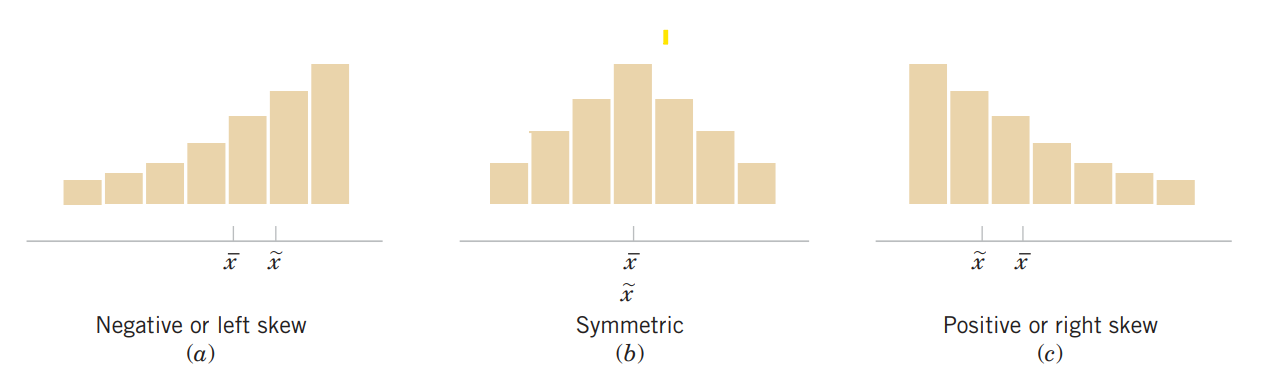
\includegraphics[keepaspectratio]{ShapeDistribution.png}}

}

\caption{\label{fig-fig22}Histograms for symmetric and skewed
distributions}

\end{figure}%

\subsection{Box-plot}\label{box-plot}

The \textbf{box plot} is a graphical display that simultaneously
describes several important features of a data set, such as
\emph{center}, \emph{spread}, departure from \emph{symmetry}, and
identification of unusual observations or \emph{outliers}.

A box plot, sometimes called \emph{box-and-whisker plots}, displays the
\textbf{three quartiles}, \textbf{the minimum/lower fence}, and
\textbf{the maximum/upper fence} of the data on a rectangular box,
aligned either horizontally or vertically.

If any value falls outside the \textbf{fences} then it will shown as a
\textbf{circle} in the box-plot.

\textbf{Example 1.11}

\section{Variable-I}

Suppose, X=\{10,15,14,18,17,12,16,15,19,21,32,12,58\}

\pandocbounded{
\includegraphics[keepaspectratio]{1Introduction_to_statistics_1_files/figure-pdf/unnamed-chunk-2-1.pdf}}

\section{Variable-II}

Suppose, Y=\{5,8,14,15,18,17,16,14,15,21,21,35,17,16,20\}

\pandocbounded{
\includegraphics[keepaspectratio]{1Introduction_to_statistics_1_files/figure-pdf/unnamed-chunk-3-1.pdf}}

\subsection{Boxplot and skewness of the
data}\label{boxplot-and-skewness-of-the-data}

When we discuss the frequency histogram we also learned about shape of
the distribution. By visual inspection of boxplot we can also tell about
the distribution shape of a variable. The following boxplots are the
typycal examples of skewness of the data.

\pandocbounded{
\includegraphics[keepaspectratio]{1Introduction_to_statistics_1_files/figure-pdf/unnamed-chunk-4-1.pdf}}

\textbf{Comparative/Parallel box-plots}

Box plots are very useful in graphical comparisons among data sets
because they have high visual impact and are easy to understand.

\begin{itemize}
\tightlist
\item
  For instance, here the \textbf{Life expectancy at birth (in year)} of
  Afghanistan, Bangladesh, India and Pakistan is compared using a
  \textbf{comparative box-plot} from 1971 to 2007.
\end{itemize}

\pandocbounded{
\includegraphics[keepaspectratio]{1Introduction_to_statistics_1_files/figure-pdf/unnamed-chunk-5-1.pdf}}

\textbf{Question:} What is/are your observation(s) from this above
comparative box-plot?\\

\section{Exercises (Practice as more as you
can)}\label{exercises-practice-as-more-as-you-can}

\textbf{1.1 Define} statistics, population, sample, descriptive and
inferential statistics.

\textbf{1.2} Define data. Discuss the types of data with example.

\textbf{1.3} What are the common measures of location? When median is
preferable to mean?

\textbf{1.4} What are the common measures of variation?

\textbf{1.5 Define} five-number summary. How to detect outliers using
quartiles?

\textbf{1.6} The data contains the overall gallons per kilometer (GpK)
of a medium-sized mobile home unit.

35, 30, 37, 35, 34, 35, 35, 42,40, 37, 42, 38, 35, 34, 35, 34, 34.

\textbf{Calculate} and \textbf{explain} Median. \textbf{Find} the value
above which 15\% GpK values lie.

\textbf{1.7} In automobile mileage and gasoline-consumption testing, 13
automobiles were road tested for 300 miles in city driving conditions.
The following data were recorded for miles-per-gallon (mpg) performance.

\begin{quote}
13.2, 14.4, 15.2, 15.3, 15.3, 15.3, 15.9, 16.0, 16.1, 16.2, 16.2, 16.7,
16.8
\end{quote}

\begin{enumerate}
\def\labelenumi{\roman{enumi})}
\item
  \textbf{Construct} a simple boxplot (in horizontal direction) of mpg.
  Are most of the automobiles' mpg relatively low?
\item
  Suppose you want to buy a new car and you don't afford enough money,
  so the car's mileage must be in \emph{bottom} 10\%. What should be the
  mileage of your car based on this data?
\item
  Suppose you want to buy a new car which mileage must be in \emph{top}
  10\%. What should be the mileage of your car based on this data?
\end{enumerate}

\textbf{1.8} The data set lists the prices (in dollars) of 20 portable
global positioning system (GPS) navigators.

\begin{quote}
128, 100, 180, 150, 200, 90, 340, 105, 85, 270, 200, 65, 230, 150, 150,
120, 130, 80, 230, 200
\end{quote}

\begin{enumerate}
\def\labelenumi{\roman{enumi})}
\item
  \textbf{Construct} a frequency distribution and percent frequency
  distribution of prices.
\item
  \textbf{Draw} a frequency histogram. What is your observation about
  price data?
\end{enumerate}

\textbf{1.9} The lengths of power failures, in minutes, are recorded in
the following table.

\begin{quote}
18, 135, 15, 90, 78, 69, 98, 102, 83, 55, 28
\end{quote}

\begin{enumerate}
\def\labelenumi{\roman{enumi})}
\item
  \textbf{Compute} sample mean and standard deviation
\item
  \textbf{Compute} sample median and IQR
\item
  If you want to be in the bottom 10\% of power failures in your
  residence, then what should be the cutoff value of power failure
  lengths in minutes?
\end{enumerate}

\textbf{1.10} Sample annual salaries (in thousands of dollars) for
entry-level electrical engineers in Boston and Chicago are listed.

\begin{quote}
\textbf{Boston} 70.4, 84.2, 58.5, 64.5, 71.6, 79.9, 88.3, 80.1, 69.9

\textbf{Chicago} 69.4, 71.5, 65.4, 59.9, 70.9, 68.5, 62.9, 70.1, 60.9
\end{quote}

\textbf{Find} the coefficient of variation for each of the two data
sets. Then \textbf{compare} the results.

\textbf{1.11} The shear strengths of 20 spot welds in a titanium alloy
are as follows:

\begin{quote}
5408 5431 5475 5442 5376 5388 5459 5422 5416 5435

5420 5429 5401 5446 5487 5416 5382 5357 5388 5457
\end{quote}

\textbf{Construct} a frequency histogram of shear strength data.
\textbf{Conclude} whether the shear strength is approximately symmetric
or not.

\textbf{1.12} The ``cold start ignition time'' of an automobile engine
is being investigated by a gasoline manufacturer. The following times
(in seconds) were obtained for a test vehicle:

\begin{quote}
1.75, 1.92, 2.62, 2.35, 3.09, 3.15, 2.53, 1.91.
\end{quote}

\textbf{Check} for outliers using the 1.5*IQR rule of cold start
ignition time.

\textbf{1.13} The cylindrical compressive strength (in MPa) was measured
for 11 beams. The results were:

\begin{quote}
38.43, 38.43, 38.39, 38.83, 38.45, 38.35, 38.43, 38.31, 38.32, 38.48,
38.50.
\end{quote}

\textbf{i) Construct} a simple boxplot and comment about the shape of
the distribution of compressive strength.

\textbf{ii) Compute} sample mean, standard deviation and coefficient of
variation (CV) compressive strength.

\textbf{1.14} The shear strengths (in N/m2) of 10 spot welds in a
titanium alloy are:

5408, 5431, 5475, 5442, 5376, 5388, 5459, 5422, 5416, 5435.

\textbf{Compute} sample mean, standard deviation and coefficient of
variation of shear strength.

\textbf{1.15} An article describes an experiment to test the yield
strength of circular tubes with caps welded to the ends. The first 18
yields (in kN) are:

\begin{quote}
96, 96, 102, 102, 102, 104, 104, 108, 126,126, 128, 128, 140, 156, 160,
160, 164,170.
\end{quote}

\textbf{Construct} a simple box-plot of yield strength. \textbf{Find}
the value above which top 10\% yield strength lie.

\textbf{1.16} The cylindrical compressive strength (in MPa) was measured
for 11 beams. The results were:

\begin{quote}
38.43, 38.43, 38.39, 38.83, 38.45, 38.35, 38.43, 38.31, 38.32, 38.48,
38.50.
\end{quote}

\begin{enumerate}
\def\labelenumi{\roman{enumi})}
\item
  \textbf{Compute} 1st quartile, 3rd quartile and IQR.
\item
  \textbf{Check} for outlier (s).
\item
  \textbf{Construct} a box-plot, \textbf{show} the outliers and
  \textbf{comment} about the symmetry of the distribution.
\end{enumerate}

\textbf{1.17} The following sample data presents the thickness (Å) of a
metal layer on 20 silicon wafers resulting from a chemical vapor
deposition (CVD) process. Scientists believe that the thickness is
usually normally distributed having a bell-shaped distribution for a
smooth process. \textbf{Construct} a frequency histogram of metal
thickness data. \textbf{Conclude} whether the process is smooth or not.

\begin{quote}
468, 459, 450, 453, 473, 454, 458, 438, 447, 463,

445, 466, 456, 434, 471, 437, 459, 445, 454, 423
\end{quote}

\bookmarksetup{startatroot}

\chapter{Probability}\label{probability}

\section{Introduction}\label{introduction}

A probability is the chance, or likelihood, that a particular event will
occur. These are examples of events representing typical
probability-type questions:

\begin{itemize}
\item
  How many customers will arrive in a super shop in next 30 minutes?
\item
  What is probability that a stock price will rise or fall?
\end{itemize}

To answer these kind of questions in the face of uncertainty we need to
study probability. To answer these type of questions which are raised in
real life; at first we have to learn some basic concepts of probability.

\section{Random experiment}\label{random-experiment}

A \textbf{random experiment} is a process leading to two or more
possible outcomes, without knowing exactly which outcome will occur.

\textbf{Example:} Tossing a coin, throwing a dice, change in the stock
prices etc.

\section{Sample space}\label{sample-space}

A \textbf{sample space} is the collection of all outcomes of a random
experiment. The sample space is usually denoted by \(S\) or Greek letter
\(\Omega\) (omega).

\textbf{Example 2.1:}

\begin{itemize}
\item
  If we toss a coin then the sample space is: \(S=\{H,T\}\)
\item
  If we toss 2 coins then the sample space is: \(S=\{HH,HT,TH,TT\}\)
\end{itemize}

\section{Event}\label{event}

An \textbf{event} is a \emph{subset} of a \emph{sample space}.

For example suppose, \(S=\{HH,HT,TH,TT\}\) and
\(A=\{ one \ \ head \ \ occurs  \}\). So, \(A=\{ HT,TH\}\).

Since \(A\) is a subset of sample space \(S\), so \(A\) is an
\emph{event}.

\section{Complement of an event}\label{complement-of-an-event}

The complement of an event A with respect to Ω is the subset of all
elements of \(\Omega\) that are not in A. We denote the complement of A
by the symbol \(A^C\).

\textbf{Example 2.2:} Consider the sample space:

\(\Omega =\{ 1,2,3,4,5,6\}\)

Let, \(A=\{1,3,5 \}\). Then the complement of \(A\) is
\(A^C=\Omega-A=\{2,4,6\}\)

\section{Mutually exclusive events}\label{mutually-exclusive-events}

The occurrence of one event means that none of the other events can
occur at the same time.

\textbf{Example}

\begin{itemize}
\item
  The variable ``Employment status'' presents mutually exclusive
  outcomes, \emph{employed} and \emph{unemployed}. An employee selected
  at random is either male or female but cannot be both.
\item
  A manufactured part is acceptable or unacceptable. The part cannot be
  both acceptable and unacceptable at the same time.
\end{itemize}

\section{Axiomatic definition of
Probability}\label{axiomatic-definition-of-probability}

The \textbf{probability} of an event \(A\) is the sum of the weights of
all sample points in \(A\). Therefore

(a) \(0 \le P(A)\le 1\) ; \(P(\phi)=0\) and \(P(\Omega)=1\).

(b) If \(A_1, A_2,A_3,...\) is a sequence of mutually exclusive events,
then

\[P(A_1\cup A_2 \cup  A_3\cup ...).=P(A_1)+P(A_2)+P(A_3)+...\]

\section{Probability of an event (Classical
approach)}\label{probability-of-an-event-classical-approach}

Suppose an event \(A\) is defined in the sample space \(\Omega\). Then
the probability of event \(A\) is defined as :

\[P(A)=\frac{n(A)}{n(\Omega)};\]

Here,

\(n(A)=\) number of outcomes favorable to event \(A\);

\(n(\Omega)=\) total number of outcomes in the sample space \(\Omega\).

\section{Probability of an event (Empirical
approach)}\label{probability-of-an-event-empirical-approach}

\textbf{Empirical Probability} is a type of probability that is
calculated based on actual observations, experiments, or historical data
rather than theoretical assumptions. It measures the likelihood of an
event occurring by analyzing past occurrences or experimental results.

\textbf{Formula for Empirical Probability:}

\[ P(E)=\frac{Number\ \ of  \ \ times \ \ the\ \  event\ \  occurs}{Total \ \ number\ \  of \ \ trials} \]

Where:

\begin{itemize}
\item
  \(P(E)\) is the probability of the event \(E\),
\item
  The numerator is the count of occurrences of the event, and
\item
  The denominator is the total number of trials or observations.
\end{itemize}

\textbf{Example 2.3:} Suppose in a class there are 30 students; 20 are
male and 10 are females. If a student is selected at random what is the
probability that he is a male?

\ul{Solution:} Let, \(A_1=\) set of male students and \(A_2=\) set of
female students. And, \(\Omega=\) set of all students

So, probability that a male student is selected is:

\[P(A_1)=\frac{n(A_1)}{n(\Omega)}=\frac{20}{30}=0.66667\approx 0.67\]

\emph{Interpretation} There is almost \(67\%\) chance that the selected
student will be male.

\textbf{Example 2.4:} If 3 books are picked at random from a shelf
containing 5 novels, 3 books of poems, and a dictionary, what is the
probability that

(a) the dictionary is selected?

(b) 2 novels and 1 book of poems are selected?

\section{Properties of Probability
Laws}\label{properties-of-probability-laws}

Probability laws have a number of properties, which can be deduced from
the axioms. Some of them are summarized below.

a) \(P(A^C)=1-P(A)\) \textbf{{[}complement rule{]}}

b) \(P(A \cap B^C )=P(A)-P(A \cap B)\) \textbf{{[}only A happens{]}}

c) \(P(A \cup B)=P(A)+P(B)-P(A \cap B)\) \textbf{{[}additive rule{]}}

d) \(P(A^C \cap B^C )=P(A∪B)^C=1-P(A \cup B)\). \textbf{{[}neither A NOR
B happens{]}}

\textbf{Example 2.5:} In a class 65\% students prefer tea and 35\%
students prefer coffee. While 15\% students prefer both tea and coffee.
If a student is selected at random from the class \textbf{find} the
probability that

\begin{enumerate}
\def\labelenumi{\roman{enumi})}
\item
  he/she prefers only coffee
\item
  he/she prefers tea or coffee
\item
  he/she prefers none (neither tea nor coffee)
\end{enumerate}

\textbf{Example} All Seasons Plumbing has two service trucks that
frequently need repair. If the probability the first truck is available
is 0.80, the probability the second truck is available is 0.60, and the
probability that both trucks are available is .30, what is the
probability neither truck is available?

\section{Conditional Probability}\label{conditional-probability}

The conditional probability of an event \(A\), \emph{given} an event
\(B\) with \(P(B) > 0\), is defined by,

\[P(A|B)=\frac{P(A\cap B)}{P(B)}\] \textbf{Example 2.6} (Walpole et al.
2017a , 9th ed., page 63): Suppose that our sample space \(\Omega\) is
the population of adults in a small town who have completed the
requirements for a college degree. We shall categorize them according to
gender and employment status. The data are given in
\textbf{?@tbl-tbl21}.

\begin{longtable}[]{@{}lccc@{}}
\caption{Categorization of the Adults in a Small Town}\tabularnewline
\toprule\noalign{}
& Employed & Unployed & Total \\
\midrule\noalign{}
\endfirsthead
\toprule\noalign{}
& Employed & Unployed & Total \\
\midrule\noalign{}
\endhead
\bottomrule\noalign{}
\endlastfoot
\textbf{Male} & 460 & 40 & 500 \\
\textbf{Female} & 140 & 260 & 400 \\
\textbf{Total} & 600 & 300 & 900 \\
\end{longtable}

A person is selected at random. What is the probability that the
selected person is:

\textbf{(i)} a Male

\textbf{(ii)} a Female and employed

\textbf{(iii)} a Male or unemployed

\textbf{(iv)} a Male given that he is employed

\section{\texorpdfstring{\textbf{The Multiplication
Rule}}{The Multiplication Rule}}\label{the-multiplication-rule}

If in an experiment the events A and B can both occur, then

\[P(A\cap B)=P(A) P(B|A) ; \ \ provided \ \ P(A)>0\]

In general, assuming that all of the conditioning events (let, 3 events)
have positive probability, we have

\[P(A_1\cap A_2\cap A_3)=P(A_1) P(A_2|A_1)P(A_3|A_1\cap A_2)\]

\textbf{Example 2.7 {[}Walpole et al. (2017a) ,} Example
2.36\textbf{{]}:} Suppose that we have a fuse box containing 20 fuses,
of which 5 are defective. If 2 fuses are selected at random and removed
from the box in succession without replacing the first, what is the
probability that both fuses are defective?

\section{Probability trees}\label{probability-trees}

Consider a sequential experiment where in the \textbf{first stage}
either \(A_1\) or \(A_2\) can be happened with some probabilities . And
in the \textbf{second stage} event \(B\) can be happened. If \(B^C\) is
the complement of \(B\) then this experiment can be shown in the
following \textbf{tree diagram.}

\begin{center}
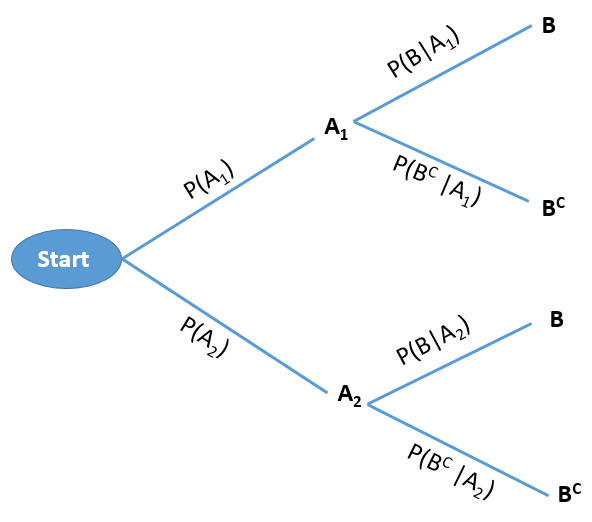
\includegraphics[width=3.8125in,height=2.64583in]{Tree.png}
\end{center}

\textbf{Example 2.8:} Two balls are drawn in succession, without
replacement, from a box containing 3 blue and 2 white balls .

i) What is the probability that both balls will be white?

\ul{Solution:} Here, two balls are drawn in succession (one by one)
without replacement. This experiment can be shown in the following tree:

\begin{center}
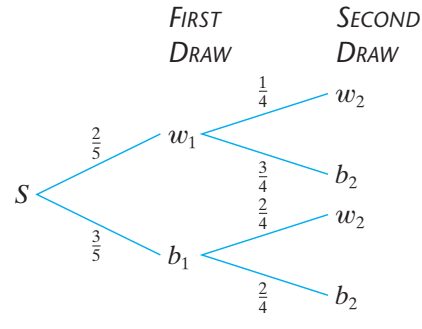
\includegraphics[width=3.27083in,height=1.86458in]{Ball_tree.png}
\end{center}

The probability of drawing a white ball on the first draw and a white
ball on the second draw (both are white) is:

\(P(w_1\cap w_2)=P(w_1) P(w_2|w_1)=(\frac {2}{5}) (\frac {1}{4})=\frac {1}{10}\)

ii) What is the probability that the second ball is white?

\ul{Solution:}

\(P(w_2)=P(w_1\cap w_2)+P(b_1\cap w_2)\)

\(=P(w_1)P(w_2|w_1)+P(b_1)P(w_2|b_1)\)

\(=(\frac{2}{5})(\frac{1}{4})+(\frac{3}{5})(\frac{2}{4})=\frac{1}{10}+\frac{3}{10}=\frac{4}{10}=\frac{2}{5}\)

\textbf{*Example 2.9 {[}Walpole et al. (2017a),} Example
2.37\textbf{{]}:} One bag contains 4 white balls and 3 black balls, and
a second bag contains 3 white balls and 5 black balls. One ball is drawn
from the first bag and placed unseen in the second bag. What is the
probability that a ball now drawn from the second bag is black?
\emph{(\textbf{Hints:} Apply probability tree)}

\textbf{Example 2.10-Radar Detection} (Bertsekas and Tsitsiklis 2008)
\textbf{:} If an aircraft is present in a certain area, radar detects it
and generates an alarm signal with probability 0.99. If an aircraft is
not present the radar generates a (false) alarm, with probability 0.10.
We assume that an aircraft is present with probability 0.05. What is the
probability of no aircraft presence and a false alarm? What is the
probability of aircraft presence and no detection?

\section{Independent events}\label{independent-events}

If two events A and B are independent, the probability that both of them
occur is equal to the product of their individual probabilities i.e.

\[P(A\cap B)=P(A) P(B)\]

\begin{itemize}
\tightlist
\item
  \textbf{Corollary:} If A and B are independent events then their
  complement events also be independent that is,
\end{itemize}

\[P(A^C\cap B^C)=P(A^C) P(B^C)\]

\begin{itemize}
\tightlist
\item
  \textbf{Independence Rule for Multiple events:}
\end{itemize}

\[P(A\cap B \cap C )=P(A) P(B) P(C) \]

\textbf{Example 2.11} (Walpole et al. 2017b, Exercise 2.89) A town has
two fire engines operating independently. The probability that a
specific engine is available when needed is 0.96.

(a) What is the probability that neither is available when needed?

(b) What is the probability that a fire engine is available when needed?

\textbf{Example} (Lind, Marchal, and Wathen 2012, 182) You take a trip
by air that involves three independent flights. If there is an 80
percent chance each specific leg of the trip is done on time, what is
the probability all three flights arrive on time?

\textbf{Example} (Lind, Marchal, and Wathen 2012, 182) The probability a
HP network server is down is .05. If you have three independent servers,
what is the probability that at least one of them is operational?

\textbf{Example} (Lind, Marchal, and Wathen 2012, 182) Twenty-two
percent of all liquid crystal displays (LCDs) are manufactured by
Samsung. What is the probability that in a collection of three
independent LCD purchases, at least one is a Samsung?

\section{System Reliability (Montgomery and Runger 2014b,
38)}\label{system-reliability-montgomery2014b-page-38}

\begin{itemize}
\tightlist
\item
  \textbf{Series circuit:} Suppose component \(L\) and \(R\) are
  connected in series from left to right . Also assume \(L\) and \(R\)
  operate ( or fail ) independently.
\end{itemize}

\begin{center}
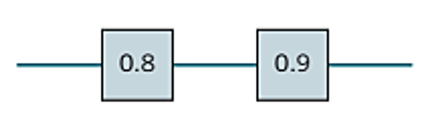
\includegraphics[width=2.40625in,height=\textheight,keepaspectratio]{Series_circuit.png}
\end{center}

The probability that the circuit operates is

\[P(L \ \ and \ \ R)=P(L \cap R)=P(L)P(R)=0.8*0.9=0.72\]

\textbf{\emph{Practical interpretation:}} Notice that the probability
that the circuit operates degrades to approximately 0.7 when all devices
are required to be functional. The probability that each device is
functional needs to be large for a circuit to operate when many devices
are connected in series.

\begin{itemize}
\tightlist
\item
  \textbf{Parallel circuit:} The following circuit operates only if
  there is a path of functional devices from left to right. The
  probability that each device functions is shown on the graph. Assume
  that devices fail independently. What is the probability that the
  circuit operates?
\end{itemize}

\begin{center}
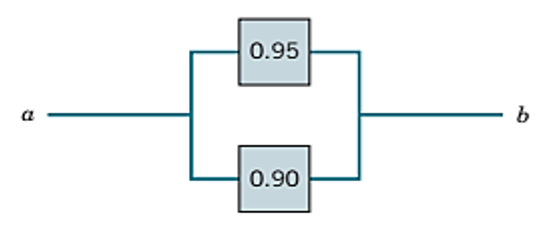
\includegraphics[width=3.21875in,height=\textheight,keepaspectratio]{Parallel_circuit.png}
\end{center}

Let \(T\) and \(B\) denote the events that the top and bottom devices
operate, respectively. There is a path if at least one device operates.
The probability that the circuit operates is

\[P(T \ \ or \ \ B) =P(T\cup B)=1-P(T^C \cap B^C)\]

\[=1-P(T^C)P(B^C)=1-(0.05)(0.10)=1-0.005=0.995\]

\textbf{\emph{Practical Interpretation:}} Notice that the probability
that the circuit operates is larger than the probability that either
device is functional. This is an advantage of a parallel architecture. A
disadvantage is that multiple devices are needed.

\textbf{Advance circuit} The following circuit operates only if there is
a path of functional devices from left to right. The probability that
each device functions is shown on the graph. Assume that devices fail
independently. What is the probability that the circuit operates?
(\textbf{Ans.:} 0.9865)\\

\begin{center}
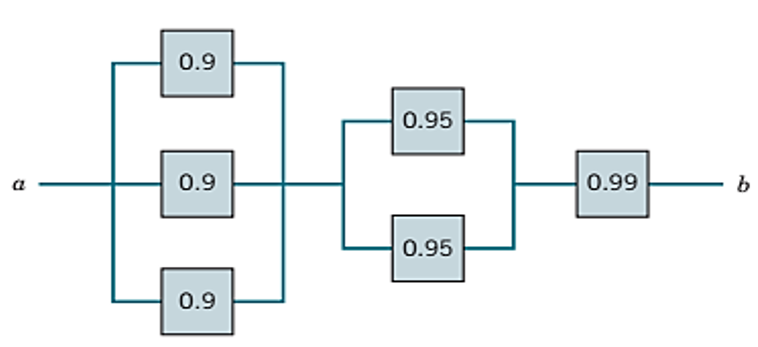
\includegraphics[width=3.76042in,height=\textheight,keepaspectratio]{Advance_circuit.png}
\end{center}

\textbf{Example} \textbf{2.12:} The following circuit operates if and
only if there is a path of functional devices from left to right. The
probability that each device functions is as shown. Assume that the
probability that a device is functional does not depend on whether or
not other devices are functional. What is the probability that the
circuit operates? (\textbf{Ans.:} 0.9293)

\begin{center}
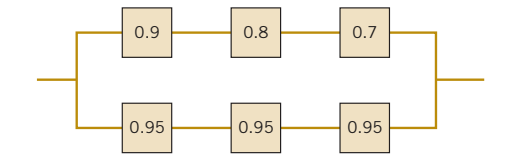
\includegraphics[width=4in,height=\textheight,keepaspectratio]{Figure2-156.png}
\end{center}

\textbf{Example 2.13:} The following circuit operates if and only if
there is a path of functional devices from left to right. The
probability that each device functions is as shown. Assume that the
probability that a device is functional does not depend on whether or
not other devices are functional. What is the probability that the
circuit operates? (\textbf{Ans.:} 0.9702)

\begin{center}
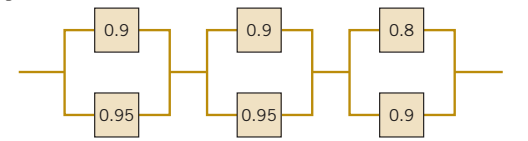
\includegraphics[width=4in,height=\textheight,keepaspectratio]{Figure2-157.png}
\end{center}

\textbf{*Example 2.14:} The following circuit operates if and only if
there is a path of functional devices from left to right. Assume devices
fail independently and that the probability of \emph{failure} of each
device is as shown. What is the probability that the circuit operates?

\begin{center}
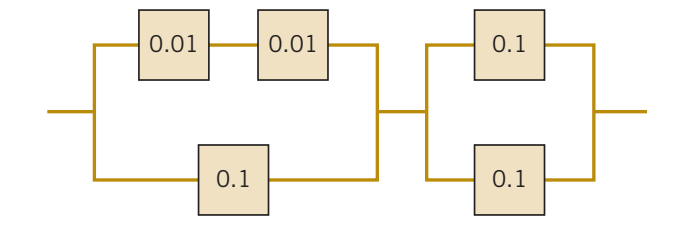
\includegraphics[width=3.64583in,height=\textheight,keepaspectratio]{Figure2-208.png}
\end{center}

\section{Total Probability Theorem and Bayes'
Rule}\label{total-probability-theorem-and-bayes-rule}

In this section, we explore some applications of conditional
probability. We start with the following theorem, which is often useful
for computing the probabilities of various events, using a
``divide-and-conquer'' approach.

\subsection{Total Probability Theorem}\label{total-probability-theorem}

Let \(A_1,...,A_n\) be disjoint events that form a partition of the
sample space (each possible outcome is included in one and only one of
the events \(A_1, . . . , A_n\)) and assume that \(P(A_i) > 0\), for all
\(i = 1,...,n\). Then, for any event \(B\), we have

\begin{center}
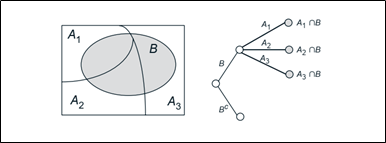
\includegraphics[width=5.61458in,height=\textheight,keepaspectratio]{Total_probability.png}
\end{center}

\[P(B)=P(A_1\cap B)+P(A_2\cap B)+....+P(A_n\cap B)\]

\[=P(A_1)P(B|A_1)+P(A_2)P(B|A_2)+....+P(A_n)P(B|A_n)\]

\textbf{Example 2.15:} Suppose that \(A_1, A_2, A_3\), and B are events
where \(A_1\), \(A_2\), and \(A_3\) are mutually exclusive and
\(P(A_1) =0.2, P(A_2) =0.5, P(A_3) =0.3\). Also given
\(P(B| A_1)=0.02, P(B|A_2)=0.05, P(B|A_3)=0.04\). Find \(P(B)\).

\subsection{Bayes' Rule/Theorem}\label{bayes-ruletheorem}

Let \(A_1,A_2,...,A_n\) be disjoint events that form a partition of the
sample space, and assume that \(P(A_i) > 0\), for all \(i\). Then, for
any event \(B\) such that \(P(B) > 0\), we have

\[P(A_i|B)=\frac{P(A_i \cap B)}{P(B)}=\frac{P(A_i)P(B|A_i)}{P(A_1)P(B|A_1)+P(A_2)P(B|A_2)+....+P(A_n)P(B|A_n)}\]

\textbf{Example 2.16} (Walpole, 9th ed, Example 2.41,page 74)\textbf{:}
In a certain assembly plant, three machines, \(B_1, B_2\), and \(B_3\),
make 30\%, 45\%, and 25\%, respectively, of the products. It is known
from past experience that 2\%, 3\%, and 2\% of the products made by each
machine, respectively, are defective. Now, suppose that a finished
product is randomly selected. What is the probability that it is
defective?

\textbf{Example 2.17 (}Walpole, 9th ed, Example 2.42)\textbf{:} With
reference to Example 2.41, if a product was chosen randomly and found to
be defective, what is the probability that it was made by machine B3?

\textbf{Example 2.18} (Walpole, 9th ed, Exercise 2.101) A paint-store
chain produces and sells latex and semigloss paint. Based on long-range
sales, the probability that a customer will purchase latex paint is
0.75. Of those that purchase latex paint, 60\% also purchase rollers.
But only 30\% of semigloss paint buyers purchase rollers. A randomly
selected buyer purchases a roller and a can of paint. What is the
probability that the paint is latex?

\textbf{Example 2.19 (Radar Detection revisited):} If an aircraft is
present in a certain area, a radar detects it and generates an alarm
signal with probability 0.99. If an aircraft is not present. the radar
generates a (false) alarm, with probability 0.10. We assume that an
aircraft is present with probability 0.05. What is the probability of no
aircraft presence and a false alarm?

\begin{enumerate}
\def\labelenumi{\roman{enumi})}
\tightlist
\item
  What is the probability that the radar generates alarm?
\item
  If the radar generates alarm, what is the probability that there was
  an aircraft?
\item
  If the radar does not generate alarm, what is the probability that
  there was not any aircraft?
\end{enumerate}

\textbf{Example 2.20}(Montgomery, 6th ed., Exercise 2-179)\textbf{:} An
e-mail filter is planned to separate valid e-mails from spam. The word
free occurs in 60\% of the spam messages and only 4\% of the valid
messages. Also, 20\% of the messages are spam. Determine the following
probabilities:

\begin{enumerate}
\def\labelenumi{(\alph{enumi})}
\tightlist
\item
  The message contains free.
\item
  The message is spam given that it contains free.
\item
  The message is valid given that it does not contain free.
\end{enumerate}

\textbf{Example 2.21:} One urn has 3 blue and 2 white balls; a second
urn has 1 blue and 3 white balls. A single fair die is rolled and if 1
or 2 comes up, a ball is drawn out of the first urn; otherwise, a ball
is drawn out of the second urn. If the drawn ball is blue, what is the
probability that it came out of the first urn? Out of the second urn?

\begin{center}
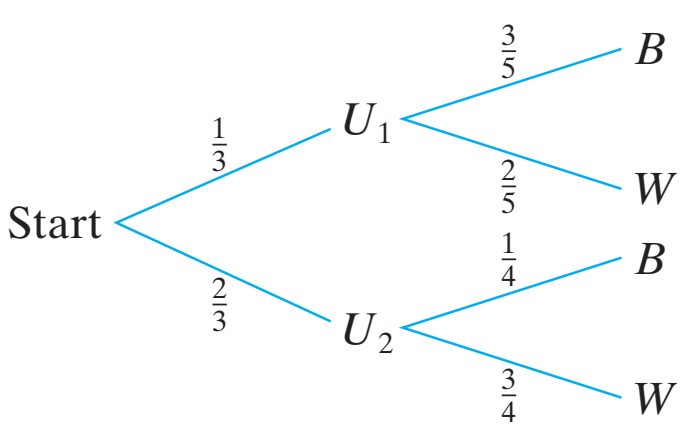
\includegraphics[width=2.6875in,height=\textheight,keepaspectratio]{Urn_model.png}
\end{center}

\textbf{*Example} \textbf{2.22:} A binary communication channel carries
data as one of two sets of signals denoted by 0 and 1. Owing to noise, a
transmitted 0 is sometimes received as a 1, and a transmitted 1 is
sometimes received as a 0. For a given channel, it can be assumed that a
transmitted 0 is correctly received with probability 0.95 and a
transmitted 1 is correctly received with probability 0.75. Also, 60\% of
all messages are transmitted as a 0. If a signal is sent, determine the
probability that:

\begin{enumerate}
\def\labelenumi{(\alph{enumi})}
\item
  a 1 was received;
\item
  a 0 was received;
\item
  an error occurred;
\item
  a 1 was transmitted given that a 1 was received ;
\item
  a 0 was transmitted given that a 0 was received.
\end{enumerate}

\bookmarksetup{startatroot}

\chapter{Random variable: Discrete}\label{random-variable-discrete}

In many situations, it is desirable to assign a numerical value to each
outcome of a random experiment. Such an assignment is called a
\textbf{random variable.}

Mathematically, a random variable is a \textbf{real-valued function} of
the experimental outcome.

\textbf{Definition:} A random variable is a function that associates a
real number with each element in the sample space.

\begin{tcolorbox}[enhanced jigsaw, bottomrule=.15mm, toprule=.15mm, title=\textcolor{quarto-callout-note-color}{\faInfo}\hspace{0.5em}{Note}, bottomtitle=1mm, colframe=quarto-callout-note-color-frame, coltitle=black, rightrule=.15mm, toptitle=1mm, colbacktitle=quarto-callout-note-color!10!white, titlerule=0mm, breakable, arc=.35mm, leftrule=.75mm, opacitybacktitle=0.6, opacityback=0, colback=white, left=2mm]

We shall use a capital letter, say \(X\), to denote a random variable
and its corresponding small letter, \(x\) in this case, for one of its
values.

\end{tcolorbox}

\textbf{Illustration:} Two balls are drawn in succession without
replacement from an urn containing 4 red balls and 3 black balls.

\begin{itemize}
\item
  Let, \(Y\) is the number of red balls.
\item
  The small letter \(y\) is the numerical value for each possible
  outcomes.
\end{itemize}

The possible outcomes and the values of \(y\) of the random variable
\(Y\) are:

\begin{longtable}[]{@{}cc@{}}
\toprule\noalign{}
\textbf{Sample space} & \(y\) \\
\midrule\noalign{}
\endhead
\bottomrule\noalign{}
\endlastfoot
\(RR\) & 2 \\
\(RB\) & 1 \\
\(BR\) & 1 \\
\(BB\) & 0 \\
\end{longtable}

Since the values of \(Y\) is determined by a random experiment so, \(Y\)
is a random variable (discrete).

\section{\texorpdfstring{\textbf{Types of random
variable}}{Types of random variable}}\label{sec-types-of-random-variable}

There are two important types of random variables, \textbf{discrete} and
\textbf{continuous}.

A \textbf{discrete random variable} is one whose possible values form a
discrete set; in other words, the values can be ordered, and there are
gaps between adjacent values. The random variable Y, just described, is
discrete.

In contrast, the possible values of a \textbf{continuous random
variable} always contain an interval, that is, all the points between
some two numbers.

\section{Discrete random variable and Probability mass
function}\label{discrete-random-variable-and-probability-mass-function}

Suppose \(X\) is a discrete random variable. The \textbf{probability
mass function (PMF)} of \(X\) can be denoted as \(f(x)\) where

\[f(x)=P(X=x)\] For each possible outcome \(x\) ; \(f(x)\) must
satisfies:

\begin{enumerate}
\def\labelenumi{\arabic{enumi}.}
\item
  \[f(x) \ge 0\]
\item
  \[\sum _x f(x)=1\]
\end{enumerate}

\subsection{The Cumulative Distribution Function of a Discrete Random
Variable}\label{the-cumulative-distribution-function-of-a-discrete-random-variable}

A function called the \textbf{cumulative distribution function (CDF)}
specifies the probability that a random variable is less than or equal
to a given value. The cumulative distribution function of the random
variable \(X\) is the function

\begin{itemize}
\tightlist
\item
  \(F(x) = P(X \le x)\)
\end{itemize}

\textbf{Example 3.1: Calculating probabilities} A certain industrial
process is brought down for recalibration whenever the quality of the
items produced falls below specifications. Let \(X\) represent the
number of times the process is recalibrated during a week, and assume
that \(X\) has the following probability mass function.

\begin{longtable}[]{@{}lccccc@{}}
\toprule\noalign{}
\(x\) & 0 & 1 & 2 & 3 & 4 \\
\midrule\noalign{}
\endhead
\bottomrule\noalign{}
\endlastfoot
\(f(x)\) & 0.35 & 0.25 & 0.20 & 0.15 & 0.05 \\
\end{longtable}

Compute the following :

i) \(P(X=2)\);

ii) \(P(X<3)\) and \(P(X>2)\);

iii) \(F(2)\)

\textbf{Example} (Walpole et al. 2017a, Example 3.8)A shipment of 20
similar laptop computers to a retail outlet contains 3 that are
defective. If a school makes a random purchase of 2 of these computers,
\textbf{find} the probability distribution for \emph{the number of
defectives}.

\textbf{\emph{Solution:}} Let \(X\) be a random variable whose values x
are the possible numbers of defective computers purchased by the school.
Then \(x\) can only take the numbers 0, 1, and 2. Now ,

\(P(X=0)=f(0)=P(N,N)=\frac{\binom{17}{2}\binom{3}{0}}{\binom{20}{2}}=\frac{136}{190}\)

\(P(X=1)=f(1)=P(D,N)=\frac{\binom{3}{1}\binom{17}{1}}{\binom{20}{2}}=\frac{51}{190}\)

\(P(X=2)=f(2)=P(D,D)=\frac{\binom{3}{2}\binom{17}{0}}{\binom{20}{2}}=\frac{3}{190}\)

Thus, the probability distribution of X is

\begin{longtable}[]{@{}lccc@{}}
\toprule\noalign{}
\(x\) & 0 & 1 & 2 \\
\midrule\noalign{}
\endhead
\bottomrule\noalign{}
\endlastfoot
\(f(x)\) & \(\frac{136}{190}\) & \(\frac{51}{190}\) &
\(\frac{3}{190}\) \\
\end{longtable}

\textbf{Example} (Baron 2019, Exercise 3.1 (a)) A computer virus is
trying to corrupt two files. The first file will be corrupted with
probability 0.4. Independently of it, the second file will be corrupted
with probability 0.3.

Compute the probability mass function (\textbf{PMF}) of \(X\), \emph{the
number of corrupted files}.

\textbf{\emph{Solution: (Will be discussed in class)}}

\subsection{Expectation (Population Mean) of discrete random
variable}\label{expectation-population-mean-of-discrete-random-variable}

Let \(X\) be a discrete random variable with probability mass function
\(f(x) = P(X = x)\).

The mean of \(X\) is given by

\[\mu=\sum_x x.f(x)\]\\
The mean of \(X\) is sometimes called the expectation, or expected
value, of X and may also be denoted by \(E(X)\) or by \(\mu\).

\textbf{Example 3.2 :} Let \(X\) represent the number of times the
process is recalibrated during a week, and assume that \(X\) has the
following probability mass function.

\begin{longtable}[]{@{}lccccc@{}}
\toprule\noalign{}
\(x\) & 0 & 1 & 2 & 3 & 4 \\
\midrule\noalign{}
\endhead
\bottomrule\noalign{}
\endlastfoot
\(f(x)\) & 0.35 & 0.25 & 0.20 & 0.15 & 0.05 \\
\end{longtable}

Compute the \textbf{mean} or \textbf{expected value} of \(X\).

\ul{Solution:}

The \textbf{expected value} of \(X\) is:

\[\mu =E[X]=\sum_{x=0}^4 x.f(x) \]

\[=0(0.35)+1(0.25)+2(0.20)+3(0.15)+4(0.05)=1.30\]

\subsection{Variance (population) of discrete random
variable}\label{variance-population-of-discrete-random-variable}

Let \(X\) be a discrete random variable with probability distribution
\(f(x)\) and mean \(\mu\). The variance of \(X\) is

\[var(X)=\sigma^2 =E[(X-\mu)^2]=E(X^2)-\mu^2\] Where,

\[E(X^2)=\sum_{x} x^2.f(x)\]\\

\textbf{Example 3.2 :} Let \(X\) represent the number of times the
process is recalibrated during a week, and assume that \(X\) has the
following probability mass function.

\begin{longtable}[]{@{}lccccc@{}}
\caption{Compute the \textbf{expected value} and \textbf{variance} of
\(X\).}\tabularnewline
\toprule\noalign{}
\(x\) & 0 & 1 & 2 & 3 & 4 \\
\midrule\noalign{}
\endfirsthead
\toprule\noalign{}
\(x\) & 0 & 1 & 2 & 3 & 4 \\
\midrule\noalign{}
\endhead
\bottomrule\noalign{}
\endlastfoot
\(f(x)\) & 0.35 & 0.25 & 0.20 & 0.15 & 0.05 \\
\end{longtable}

\ul{Solution:} From Example 3.1, we have

Expected value of \(X\) is \(\mu =E(X)=1.30\)

Now, \[E(X^2)=\sum_{x=0}^4 x^2.f(x)\]

\(=0^2(0.35)+1^2 (0.25)+2^2 (0.20)+3^2 (0.15)+4^2 (0.05)\)

\(=3.20\)

Hence, \(var(X)=\sigma^2 =E(X^2)-\mu^2=3.20-(1.30)^2=1.51\)

\begin{itemize}
\item
  The standard deviation is the square root of the variance:

  \(\sigma=\sqrt {var(X)}\)
\end{itemize}

\begin{tcolorbox}[enhanced jigsaw, bottomrule=.15mm, toprule=.15mm, title=\textcolor{quarto-callout-note-color}{\faInfo}\hspace{0.5em}{Properties of E(.) and var(.)}, bottomtitle=1mm, colframe=quarto-callout-note-color-frame, coltitle=black, rightrule=.15mm, toptitle=1mm, colbacktitle=quarto-callout-note-color!10!white, titlerule=0mm, breakable, arc=.35mm, leftrule=.75mm, opacitybacktitle=0.6, opacityback=0, colback=white, left=2mm]

If \(a\) and \(b\) are constants, then

a) \(E(b)=b\)

b) \(E(aX+b)=aE(X)+b\)

c) \(var(b)=0\)

d) \(var(aX+b)=a^2 \ \ var (X)\)

\end{tcolorbox}

\textbf{Example} Computer chips often contain surface imperfections. For
a certain type of computer chip, the probability mass function of the
number of defects X is presented in the following table.

\begin{longtable}[]{@{}lccccc@{}}
\toprule\noalign{}
\(x\) & \textbf{0} & \textbf{1} & \textbf{2} & \textbf{3} &
\textbf{4} \\
\midrule\noalign{}
\endhead
\bottomrule\noalign{}
\endlastfoot
\(f(x)\) & 0.4 & 0.3 & 0.15 & 0.1 & 0.05 \\
\end{longtable}

a. Find \(P(X \le 2)\).

b. Find \(P(X > 1)\).

c. Find expected value/average of \(X\).

d. Find variance and standard deviation of \(X\).

e. Also find \(E(2X+5)\) and \(var(2X+5)\).

\section{Bernoulli r.v}\label{bernoulli-r.v}

Bernoulli r.v comes from \textbf{Bernoulli trial-}a trial which has
\textbf{TWO} possible outcomes (\emph{success} or \emph{failure}).

Consider the toss of a \textbf{biased coin}, which comes up a head with
probability \(p\), and a tail with probability \(1 - p\). The
\textbf{Bernoulli random variable} takes the two values 1 and 0,
depending on whether the outcome is a head or a tail:

\[X=1 ; if \ \  a \ \ head,\\
X=0 ;  if\ \  a \ \ tail.\]

Then the PMF of \(X\) is:

\begin{itemize}
\tightlist
\item
  \textbf{PMF}:
\end{itemize}

\begin{equation}\phantomsection\label{eq-bernoulli}{P(X=x)=f(x)=p^x(1-p)^{1-x}; \ \ x=0,1}\end{equation}

\begin{itemize}
\item
  \textbf{Mean}: \(\mu=E(X)=p\)
\item
  \textbf{Variance}: \(\sigma^2 =E(X-\mu)^2=E(X^2)-\mu^2=p(1-p)\)
\end{itemize}

For all its simplicity, the Bernoulli random variable is very important.
In practice, it is used to model generic probabilistic situations with
just two outcomes, such as:

(a) The state of a telephone at a given time that can be either free or
busy.

(b) A person who can be either healthy or sick with a certain disease.

(c) The preference of a person who can be either for or against a
certain political candidate.

Furthermore, by combining multiple Bernoulli random variables, one can
construct more complicated random variables.

\begin{tcolorbox}[enhanced jigsaw, bottomrule=.15mm, toprule=.15mm, title=\textcolor{quarto-callout-note-color}{\faInfo}\hspace{0.5em}{Derivation of Mean and Variance of Bernoulli r.v}, bottomtitle=1mm, colframe=quarto-callout-note-color-frame, coltitle=black, rightrule=.15mm, toptitle=1mm, colbacktitle=quarto-callout-note-color!10!white, titlerule=0mm, breakable, arc=.35mm, leftrule=.75mm, opacitybacktitle=0.6, opacityback=0, colback=white, left=2mm]

\textbf{Mean:}

\[E(X)=\sum_{x=0}^1 x\cdot f(x)=(0) f(0)+(1)f(1)=0+1\cdotp p=p\]

\textbf{Variance:}

\(Var(X)=E(X^2)-[E(X)]^2=p-p^2=p(1-p)\)

\end{tcolorbox}

\section{Binomial r.v}\label{binomial-r.v}

In a Binomial experiment , the \textbf{Bernoulli trial} is repeated
\(n\) times with the following conditions:

a) The trials are independent

b) In each trial \(P(success)=p\) remains constant

Suppose \(X=number \ \ of \ \ successs \ \ in \ \ n\ \ trials\). Then
\(X\) is called a \textbf{Binomial r.v} or follows \textbf{Binomial
distribution.}

\textbf{PMF:}
\begin{equation}\phantomsection\label{eq-binomial}{P(X=x)=f(x)=\binom {n}{x} p^x (1-p)^{n-x} ; x=0,1,2,...,n}\end{equation}

\textbf{CDF}: \(P(X\le x)=F(x)=f(0)+f(1)+...+f(x)\)

\textbf{Properties}

\textbf{a)}
\(\sum_{x=0}^n f(x)=\sum_{x=0}^n \binom {n}{x} p^x (1-p)^{n-x}\)

\textbf{b) Mean:} \(E(X)=np\)

\textbf{c) Variance:} \(Var(X)=np(1-p)\)

\ul{\textbf{We write}} \(X\sim Bin (n,p)\)

\textbf{Illustration}

\begin{itemize}
\tightlist
\item
  Consider an experiment of tossing a biased coin 3(number of trials, n)
  times.
\item
  Tosses are \emph{independent}, each toss has only \textbf{TWO}
  Outcomes-\emph{Head (Success)} and \emph{Tail (Failure)}
\end{itemize}

\textbf{This type of trial is called the \emph{Bernoulli Trial}}

\begin{itemize}
\tightlist
\item
  Suppose, \(P(H)=p\) and remain constant in each toss, consequently,
  \(P(T)=1-p=q\) (let).
\end{itemize}

\textbf{Suppose},
\(X=\# \ \ of\ \ head\ \ (successes)\ \  in\ \ 3\ \ tosses\)

Now, what is the probability that, we will have \textbf{exactly 2 heads
(success) in 3 tosses?}

\textbf{That is,} \(P(X=2)=?\)

Now, this can happen in the following ways:

\[P(X=2)=P(HHT)+P(HTH)+P(THH)\]
\[=P(H)P(H)P(T)+P(H)P(T)P(H)+P(T)P(H)P(H)\] {[}\emph{Since tosses are
independent}{]}

\[=p.p.q+p.q.p+q.p.p\] \[=p^2 q+p^2 q+p^2 q=3p^2 q\]
\[\therefore P(X=2)=\binom{3}{2}p^2q^{3-2}\] If, \(p=0.6\) is given,
then we can easily compute \(P(X=2)=f(2)\). Now, if we repeat the toss
10 times \((n=10)\), with \(P(H)=p\), what is the value of
\(P(X=3)=f(3)\)?

\begin{tcolorbox}[enhanced jigsaw, bottomrule=.15mm, toprule=.15mm, title=\textcolor{quarto-callout-note-color}{\faInfo}\hspace{0.5em}{Note}, bottomtitle=1mm, colframe=quarto-callout-note-color-frame, coltitle=black, rightrule=.15mm, toptitle=1mm, colbacktitle=quarto-callout-note-color!10!white, titlerule=0mm, breakable, arc=.35mm, leftrule=.75mm, opacitybacktitle=0.6, opacityback=0, colback=white, left=2mm]

\begin{itemize}
\item
  \(n\) and \(p\) are said to be the \emph{parameters} of the Binomial
  distribution.
\item
  \(f(x)=F(x)-F(x-1)\) i.e \(f(3)=F(3)-F(2)\)
\item
  If \(Y=number \ \ of \ \ failures\ \ in \ \ n\ \ trials\) then
  \(Y\sim Bin(n,1-p)\)
\end{itemize}

\end{tcolorbox}

\begin{tcolorbox}[enhanced jigsaw, bottomrule=.15mm, toprule=.15mm, title=\textcolor{quarto-callout-note-color}{\faInfo}\hspace{0.5em}{Relation between Bernoulli r.v and Binomial r.v}, bottomtitle=1mm, colframe=quarto-callout-note-color-frame, coltitle=black, rightrule=.15mm, toptitle=1mm, colbacktitle=quarto-callout-note-color!10!white, titlerule=0mm, breakable, arc=.35mm, leftrule=.75mm, opacitybacktitle=0.6, opacityback=0, colback=white, left=2mm]

A \textbf{Binomial Random Variable} Is a \textbf{Sum of Bernoulli Random
Variables}

Let, \(Y_i\) is a Bernoulli r.v appeared in \(i^{th}\) Bernoulli trial.
If we conduct \(n\) independent Bernoulli trials then we have \(n\)
independent Bernoulli r.vs such as \(Y_1, Y_2, ..., Y_n\). Each \(Y_i\)
has values of either \(1\) or \(0\).

Now if \(X\) is a Binomial r.v then,

\[ X=Y_1+Y_2+...+Y_n =\sum_{i=1}^n Y_i \]

\end{tcolorbox}

\begin{tcolorbox}[enhanced jigsaw, bottomrule=.15mm, toprule=.15mm, title=\textcolor{quarto-callout-note-color}{\faInfo}\hspace{0.5em}{Derivation of Mean and Variance of Binomial r.v}, bottomtitle=1mm, colframe=quarto-callout-note-color-frame, coltitle=black, rightrule=.15mm, toptitle=1mm, colbacktitle=quarto-callout-note-color!10!white, titlerule=0mm, breakable, arc=.35mm, leftrule=.75mm, opacitybacktitle=0.6, opacityback=0, colback=white, left=2mm]

From previous note, we know if \(Y_i\) is a Bernoulli r.v then

\(E(Y_i)=p\) and \(Var(Y_i)=p(1-p)\)

\emph{So, the mean of Binomial r.v that is}

\[ E(X)=E(Y_1+Y_2+...+Y_n) \]

\[ =E(Y_1)+E(Y_2)+...+E(Y_n) \]

\[ =p+p+...+p=np \]

\emph{Now, the variance of} \(X\) \emph{is:}

\[ Var(X)=Var(Y_1+Y_2+...+Y_n) \]

\[ =Var(Y_1)+Var(Y_2)+...+Var(Y_n) \]

\[ =p(1-p)+p(1-p)+...+p(1-p)=np(1-p) \]

\end{tcolorbox}

\textbf{Probability plot of binomial r.v for different values of} \(p\)
and shape characteristics

\pandocbounded{
\includegraphics[keepaspectratio]{3Random_variable_3_files/figure-pdf/unnamed-chunk-1-1.pdf}}

\textbf{Finding Binomial probability manually}

Suppose, \(X\sim Binom(n,p)\); where \(n=5\) and \(p=0.6\). Find,
\emph{(i)} \(P(X=2)\) \emph{(ii)} \(P(X \le 2)\) \emph{(iii)}
\(P(X\ge3)\).

\textbf{\emph{Solution:}}

\textbf{PMF of} \(X\):
\(P(X=x)=f(x)=\binom{5}{x} 0.6^x (0.4)^{5-x} \ \ ;x=0,1,2,...,5\)

\emph{(i)} \(P(X=2)=f(2)=\binom{5}{2} 0.6^2 (0.4)^{5-2}=0.2304\)

\emph{(ii)}
\(P(X \le 2)=F(2)=f(0)+f(1)+f(2)=0.0102+0.0768+0.2304=0.3174\)

\emph{(iii)} \(P(X \ge 3)=f(3)+f(4)+f(5)=0.6826\)

\textbf{\emph{Alternative:(iii)}}

\(P(X \ge 3)=1-P(X< 3)=1-P(X \le 2)=1-F(2)=1-0.3174=0.6826\)

\textbf{Finding Binomial probability using Binomial Table}

In the end of any Statistics book there are some \textbf{Probability
Distribution Table}. We can use these table to compute the required
probability for \emph{specific values of the parameters} of certain
probability distribution. Here I share the 1st page of \textbf{Binomial
distribution table} (Baron 2019).

\pandocbounded{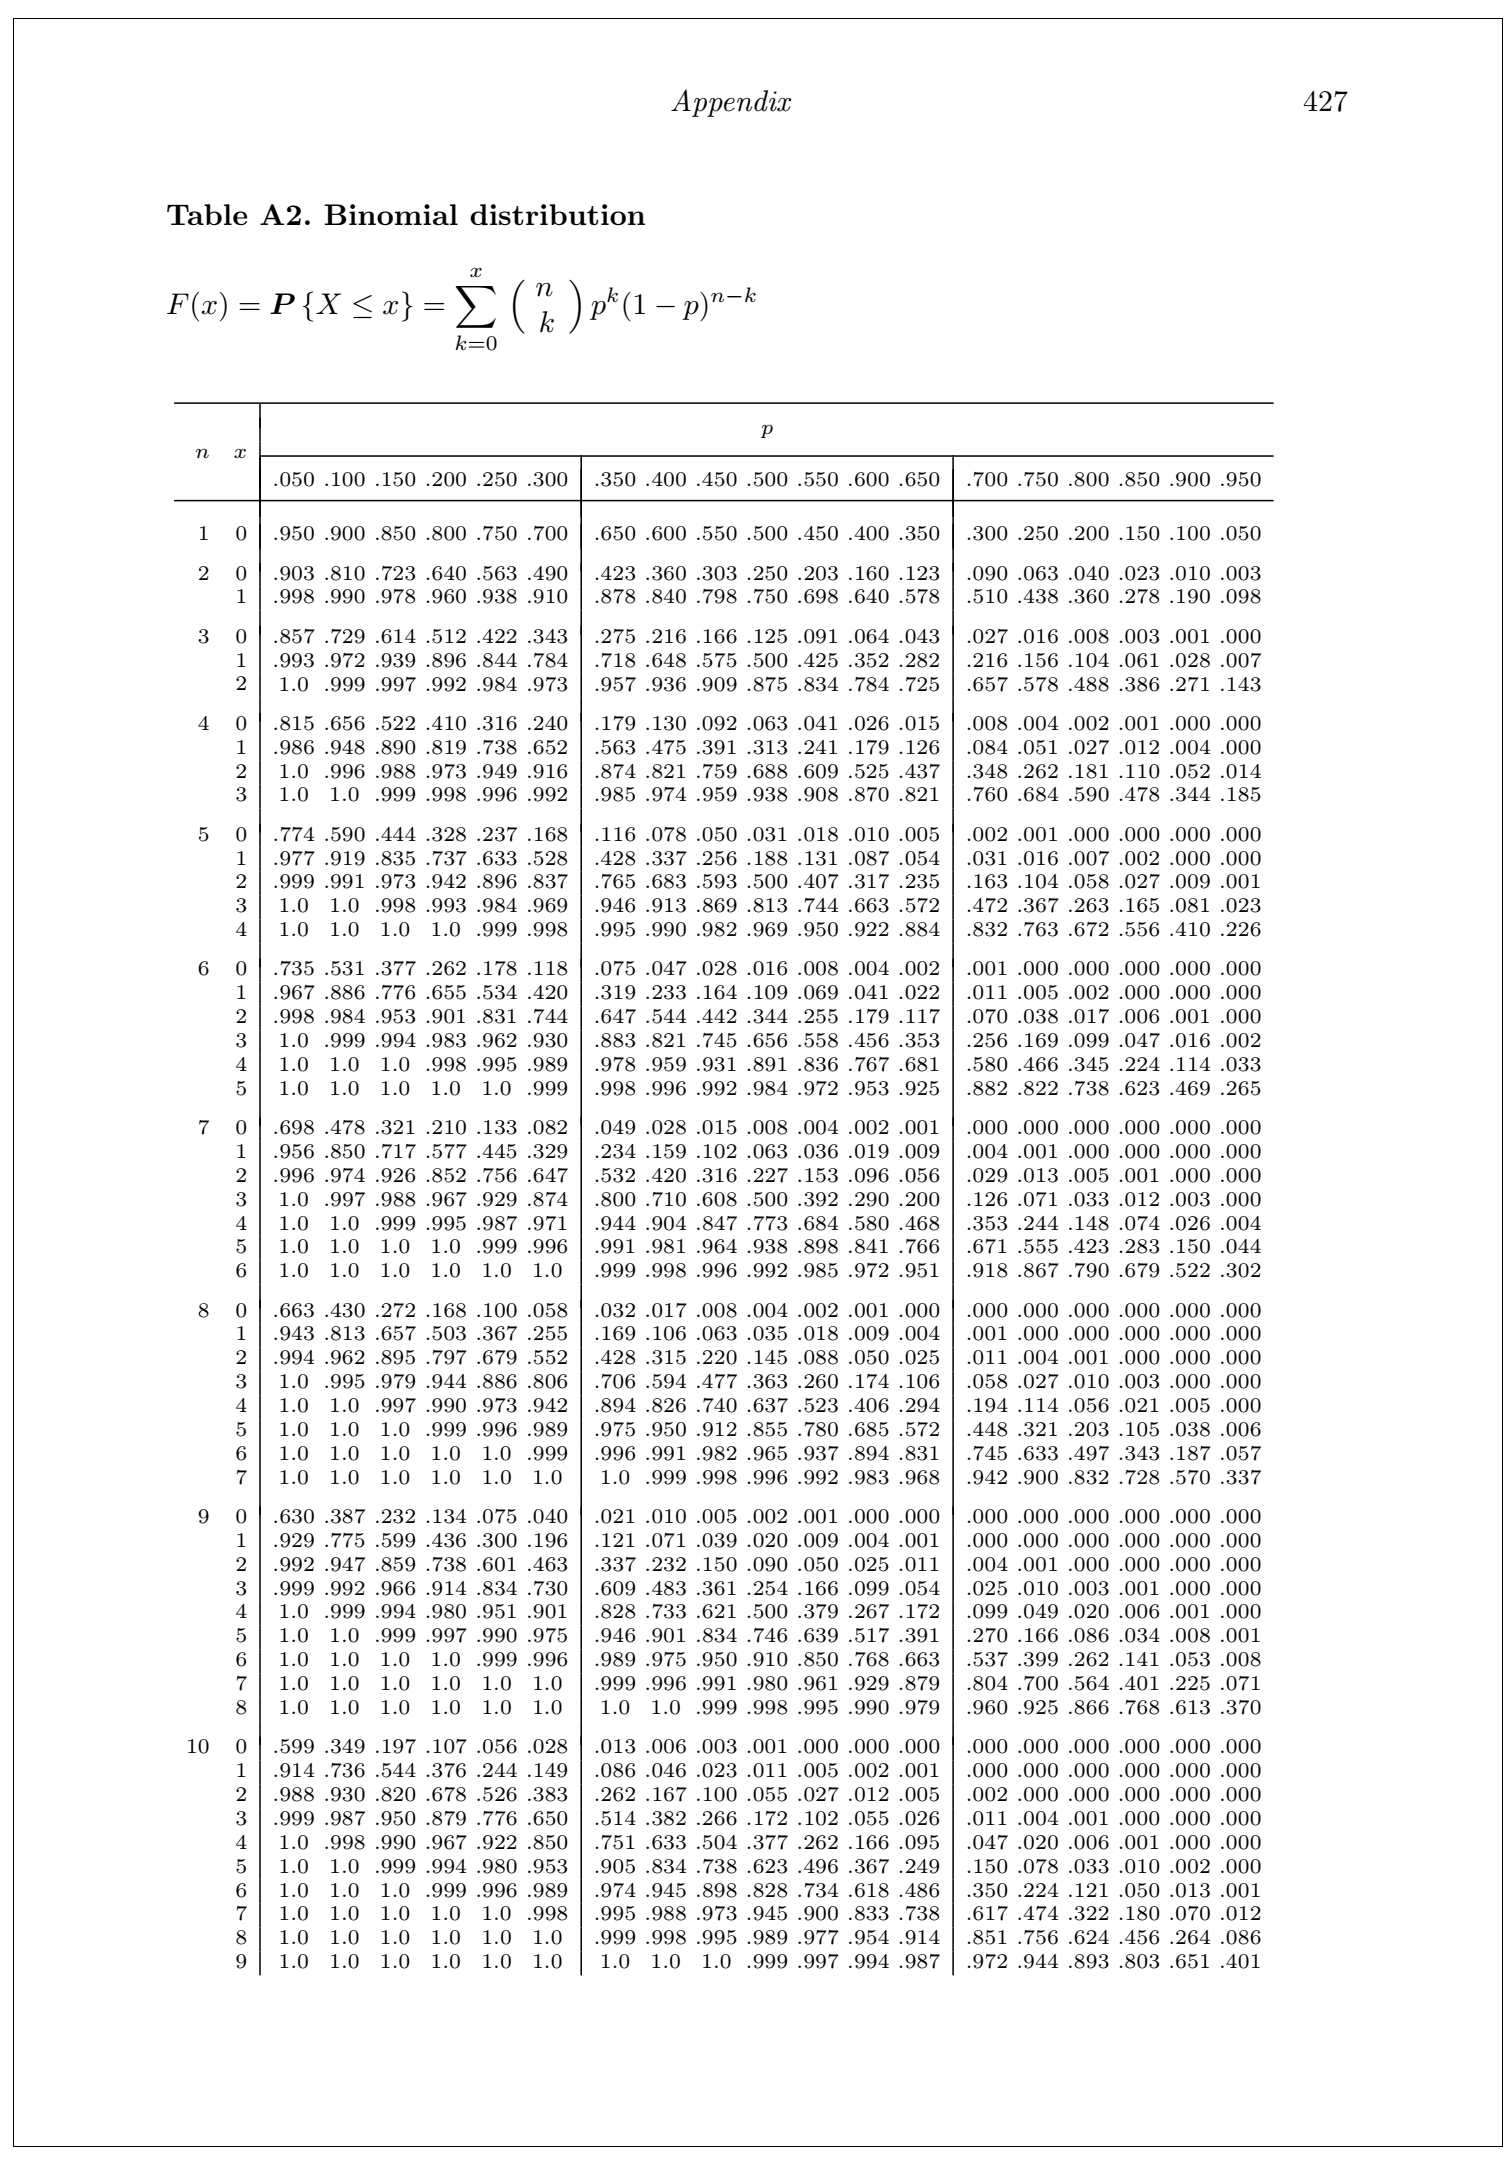
\includegraphics[keepaspectratio]{Binomial distribution_1st page.png}}

\textbf{Suppose}, \(X\sim Binom(n,p)\); where \(n=5\) and \(p=0.6\).
Find, \emph{(i)} \(P(X=2)\) \emph{(ii)} \(P(X \le 2)\) \emph{(iii)}
\(P(X \ge 3)\) using \textbf{Table}.

\textbf{\emph{Solution:}}

\emph{(i)} \(P(X=2)=f(2)=F(2)-F(1)=0.3174-0.0870=0.2304\).

\emph{(ii)} \(P(X\le 2=F(2)=0.3174\)

\emph{(iii)} \(P(X \ge 3)=1-P(X< 3)=1-F(2)=1-0.3174=0.6826\)

\textbf{Exercise}(Walpole et al. 2017a)

\textbf{5.9} In testing a certain kind of truck tire over rugged
terrain, it is found that 25\% of the trucks fail to complete the test
run without a blowout. Of the next 15 trucks tested, find the
probability that: (a) from 3 to 6 have blowouts; (b) fewer than 4 have
blowouts; (c) more than 5 have blowouts.

\emph{\textbf{Solution}:}

Let, \emph{X= number of trucks that have blowouts}

Given, \(n=15; \ \ p=Pr(blowout)=0.25; \ \ q=1-p=0.75\). Hence,
\(X\sim Binom(n=15, p=0.25)\), that is:

\[P(X=x)=f(x)=\binom{15}{x}(0.25)^x (0.75)^{15-x}; x=0,1,2,...,15.\]

Now,

\textbf{(a)}
\(P(3\le X\le 6)=f(3)+f(4)+f(5)+f(6)\)=0.225+0.225+0.165+0.092=0.707.

\textbf{\emph{Alternative:}}
\(P(3\le X\le 6)=F(6)-F(2)=0.943-0.236=0.707\) {[}from \textbf{Table}{]}

\textbf{(b)}
\(P(X<4)=f(0)+f(1)+f(2)+f(3)\)=0.013+0.067+0.156+0.225=0.461.

\textbf{\emph{Alternative:}} \(P(X< 4)=F(3)=0.461\) {[}from
\textbf{Table A2}{]}

\textbf{(c)} \(P(X > 5)=1-P(X \le 5)=1-F(5)\)=0.148

\textbf{5.12} A traffic control engineer reports that 75\% of the
vehicles passing through a checkpoint are from within the state. What is
the probability that fewer than 4 of the next 9 vehicles are from out of
state?

\textbf{5.16} Suppose that airplane engines operate independently and
fail with probability equal to 0.4. Assuming that a plane makes a safe
flight if at least one-half of its engines run, determine whether a
4-engine plane or a 2-engine plane has the higher probability for a
successful flight.

\textbf{5.25} Suppose that for a very large shipment of
integrated-circuit chips, the probability of failure for any one chip is
0.10. Assuming that the assumptions underlying the binomial
distributions are met, find the probability that at most 3 chips fail in
a random sample of 20.

\textbf{Exercise}(Montgomery and Runger 2014c)

\textbf{3-93} Let \(X\) be a binomial random variable with \(p = 0.1\) .
and \(n = 10\). Calculate the following probabilities from the binomial
probability mass function and from the binomial table in Appendix A and
compare results. (a) \(P(X\le 2)\) (b) P(X\textgreater8) (c) P(X = 4)
(d) \(P(5 \le X \le7)\)

\textbf{3-115} The probability that a visitor to a Web site provides
contact data for additional information is 0.01. Assume that 1000
visitors to the site behave independently. Determine the following
probabilities: (a) No visitor provides contact data. (b) Exactly 10
visitors provide contact data. (c) More than 3 visitors provide contact
data

\textbf{Exercise}(Baron 2019)

\textbf{3.21.} A lab network consisting of 20 computers was attacked by
a computer virus. This virus enters each computer with probability 0.4,
independently of other computers. Find the probability that it entered
at least 10 computers.

\textbf{3.22.} Five percent of computer parts produced by a certain
supplier are defective. What is the probability that a sample of 16
parts contains more than 3 defective ones?

\emph{And so on\ldots.}

\section{Geometric r.v}\label{geometric-r.v}

The number of Bernoulli trials needed to get the first success has
Geometric distribution.

Let \(X\) be the number of trials needed to get the \emph{first}
success.

\textbf{PMF:}

\(P(X=x)=P(the\ \ 1^{st} \ \ success \ \ occurs \ \ in \ \ the \ \ x^{th\ \ trial})\)

\begin{equation}\phantomsection\label{eq-geometric}{f(x)=(1-p)^{x-1} p\ \ ;x=1,2,..., \infty}\end{equation}

\textbf{Properties}

a) \(\sum_{x=1}^\infty f(x)=\sum_{x=1}^\infty (1-p)^{x-1}p=1\)

b) \(E(X)=\frac{1}{p}\)

c) \(Var(X)=\frac{1-p}{p^2}\)

\ul{We write,} \(X\sim Geom(p)\)

\textbf{Probability plot for different values of} \(p\)

\pandocbounded{
\includegraphics[keepaspectratio]{3Random_variable_3_files/figure-pdf/unnamed-chunk-4-1.pdf}}

The probability plot illustrates that as the value of (\(p\)) increases,
the likelihood of achieving the first success at an earlier trial also
increases.

\textbf{Memorylessness property of Geometric distribution}

Let \(X\) be the number of trials needed to get the \emph{first} success
and \(X\sim Geom(p)\) .Suppose that we have been watching the process
for \(n\) trials and no success has been recorded. What is the
probability that in additional \(k\) trials we will observe the
\emph{first} success? Mathematically,

\[P(X=n+k|X>n)=?\]

It can be shown that:

\[P(X=n+k|X>n)=P(X=k)\]

It implies that the probability of needing \(k\) more trials, given that
we've already had \(n\) failures, is the same as the original
probability of needing \(k\) trials to get the \emph{first} success.
This is known as \textbf{memorylessness} \textbf{property.}

\hfill\break
\textbf{Real life examples}

\begin{itemize}
\item
  A search engine goes through a list of sites looking for a given key
  phrase. Suppose the search terminates as soon as the key phrase is
  found. The number of sites visited is Geometric.
\item
  A hiring manager interviews candidates, one by one, to fill a vacancy.
  The number of candidates interviewed until one candidate receives an
  offer has Geometric distribution.
\end{itemize}

\textbf{Example 5.15 (Walpole):} For a certain manufacturing process, it
is known that, on the average, 1 in every 100 items is defective. What
is the probability that the fifth item inspected is the first defective
item found?

\textbf{Example 5.16 (Walpole):} At a ``busy time,'' a telephone
exchange is very near capacity, so callers have difficulty placing their
calls. It may be of interest to know the number of attempts necessary in
order to make a connection. Suppose that we let \emph{p} = 0\emph{.}05
be the probability of a connection during a busy time. \emph{We are
interested in knowing the probability that 5 attempts are necessary for
\textbf{a successful call.}}

Quite often, in applications dealing with the geometric distribution,
the mean and variance are important. For example, in \textbf{Example
5.16,} the \emph{expected} number of calls necessary to make a
connection is quite important. So, we can easily compute mean and
variance of a Geometric r.v.

\textbf{Exercise 5.55 (Walpole)} The probability that a student pilot
passes the written test for a private pilot's license is 0.7. Find the
probability that a given student will pass the test

(a) on the third try;

(b) before the fourth try

\textbf{Exercise 3.24 (Michael Baron).} An internet search engine looks
for a certain keyword in a sequence of independent web sites. It is
believed that 20\% of the sites contain this keyword. Compute the
probability that the search engine had to visit at least 5 sites in
order to find the first occurrence of a keyword.

\textbf{A memoryless Customer Service Call center}

A customer calls a tech support center, which takes independent attempts
to resolve an issue. On each call, there is a 20\% chance that the issue
is resolved.

\begin{enumerate}
\def\labelenumi{(\alph{enumi})}
\tightlist
\item
  What is the probability that the issue will be resolved after the 4th
  call?
\item
  Suppose the customer has already called 4times and the issue is still
  unresolved. What is the probability that it will still take more than
  3 additional calls to get the issue resolved?
\item
  Explain why the answer in (b) makes sense in terms of the memoryless
  property.
\end{enumerate}

\begin{tcolorbox}[enhanced jigsaw, bottomrule=.15mm, toprule=.15mm, title=\textcolor{quarto-callout-note-color}{\faInfo}\hspace{0.5em}{Derivation and proofs related to Geometric distribution}, bottomtitle=1mm, colframe=quarto-callout-note-color-frame, coltitle=black, rightrule=.15mm, toptitle=1mm, colbacktitle=quarto-callout-note-color!10!white, titlerule=0mm, breakable, arc=.35mm, leftrule=.75mm, opacitybacktitle=0.6, opacityback=0, colback=white, left=2mm]

\textbf{1) Memorylessness property}

\textbf{\emph{Proof:}}

PMF of Geometric r.v is : \(f(x)=q^{x-1} p \ \ ; x=1,2,...,\infty\) with
\(q=1-p\).

Now,

\(P(X=n+k|X>n)=\frac{P(\{X=n+k\} \cap  \{X>n\} )}{P(X>n)}=\frac{P(X=n+k)}{P(X>n)}\)

\(=\frac{q^{n+k-1}}{q^n (1-q)^{-1}}=\frac{q^{k-1}}{p^{-1}}=q^{k-1}p=P(X=k)\)

\(\therefore P(X=n+k|X>n)=P(X=k)\)\\

\textbf{2) Mean of geometric distribution}

Remember the geometric series :

\(1+q+q^2+q^3+....=\sum_{x=0}^\infty q^{x}=\frac{1}{1-q}=(1-q)^{-1}\)

Now,

\[\frac{d}{dq} \sum_{x=0}^{\infty} q^{x}=\frac{d}{dq}(1-q)^{-1}\]

\[Or,\sum_{x=1}^{\infty} xq^{x-1}=(1-q)^{-2}\ \ ...(A)\]

So,
\(E(X)=\sum_{x=1}^{\infty} x\cdot q^{x-1} p=p\sum_{x=1}^{\infty} x\cdot q^{x-1}=p(1-q)^{-2}\)

\(=pp^{-2}=p^{-1}=\frac{1}{p}\)

\textbf{3) Variance}

\(Var(X)=E(X^2)-[E(X)]^2=E[X(X-1)]+E(X)-[E(X)]^2 \ \ ...(B)\)

To derive the variance of geometric distribution, differentiate (A)
w.r.t \(q\) again. After some manipulation and using (B) we will have

\[Var(X)=\frac{1-p}{p^2}\]

\end{tcolorbox}

\section{Poisson r.v}\label{poisson-r.v}

The number of events occur randomly in an interval or in a region
usually follows Poisson distribution. A famous French mathematician
\emph{SimB4eon-Denis Poisson} (1781--1840) first introduced this
distribution.

\textbf{Example}

The Poisson distribution may be useful to model variables like:

\begin{itemize}
\tightlist
\item
  The \emph{no. of calls} arrive at a customer care in \emph{15 minites}
\item
  The \emph{no. of arrivals} at a car wash in \emph{one hour}
\item
  The \emph{no. of repairs} needed in \emph{10 miles} of highway
\item
  The \emph{no. of leaks} in \emph{100 miles} of pipeline etc.
\end{itemize}

Usually Poisson distribution is used to evaluate probability of
``\emph{Rare}'' event.

The probability mass function of the Poisson random variable \(X\),
representing the \emph{number of outcomes} occurring in a given time
interval denoted by \(t\), is:

\begin{itemize}
\tightlist
\item
  \textbf{PMF}:
\end{itemize}

\begin{equation}\phantomsection\label{eq-poisson}{P(X=x)=f(x)=\frac{e^{-\lambda t}(\lambda t)^x}{x!}; \ \ x=0,1,2,...,\infty.}\end{equation}

Here, \(\lambda\) is called \emph{arrival rate} or \emph{average number
of occurrences} in long-run. And only \emph{parameter} of Poisson
distribution.

\begin{itemize}
\item
  \textbf{Mean}: \(\mu=E(X)=\lambda t\)
\item
  \textbf{Variance}: \(\sigma^2 =\lambda t\)
\item
  \textbf{We write:} \(X\sim Pois(\lambda t)\)
\end{itemize}

\textbf{N.B}: The mean and variance of Poisson random random variable
are \emph{identical}. This is the \emph{unique property} of Poisson r.v.

\textbf{Probability of plot of poisson r.v for different values of}
\(\lambda\) (for a fixed interval \(t=1\))

\pandocbounded{
\includegraphics[keepaspectratio]{3Random_variable_3_files/figure-pdf/unnamed-chunk-5-1.pdf}}

We can see that, for small \(\lambda\) the distribution of Poisson r.v
is positively skewed and as the value of \(\lambda\) increases the
distribution tends to symmetry.

\textbf{Finding Poisson probability}

Consider a discrete r.v say \(X\sim Pois(\lambda t)\). Suppose,
\(\lambda =1.5\) and \(t=2\). Find, (i) P(X=4) (ii)\(P(X \le 2)\) (iii)
\(P(X\ge3)\).

\textbf{\emph{Solution}}:

\textbf{PMF} of \(X\):
\(P(X=x)=f(x)=\frac{e^{-\lambda t}(\lambda t)^x}{x!}; x=0,1,...,\infty.\)

\textbf{(i)} For \(t=2\) , \(\mu=\lambda t=1.5*2=3\).

So, \(P(X=4)=f(4)=\frac{e^{-3}(3)^4}{4!}=0.1680\)

\textbf{(ii)}
\(P(X\le2)=\sum_{x=0}^{2}f(x)=\sum_{x=0}^{2}\frac{e^{-3}(3)^x}{x!}=e^{-3}[\frac{3^0}{0!}+\frac{3^1}{1!}+\frac{3^2}{2!}]=0.4232\)

\textbf{(iii)} \(P(X \ge 3)=1-P(X< 3)=1-P(X\le 2)=1-0.423=0.5768\)

\textbf{Finding Poisson probability using Table}

We can use Poisson distribution table to compute Poisson probabilities.
Here I share the 1st page of \textbf{Poisson distribution table} (Baron
2019).

\pandocbounded{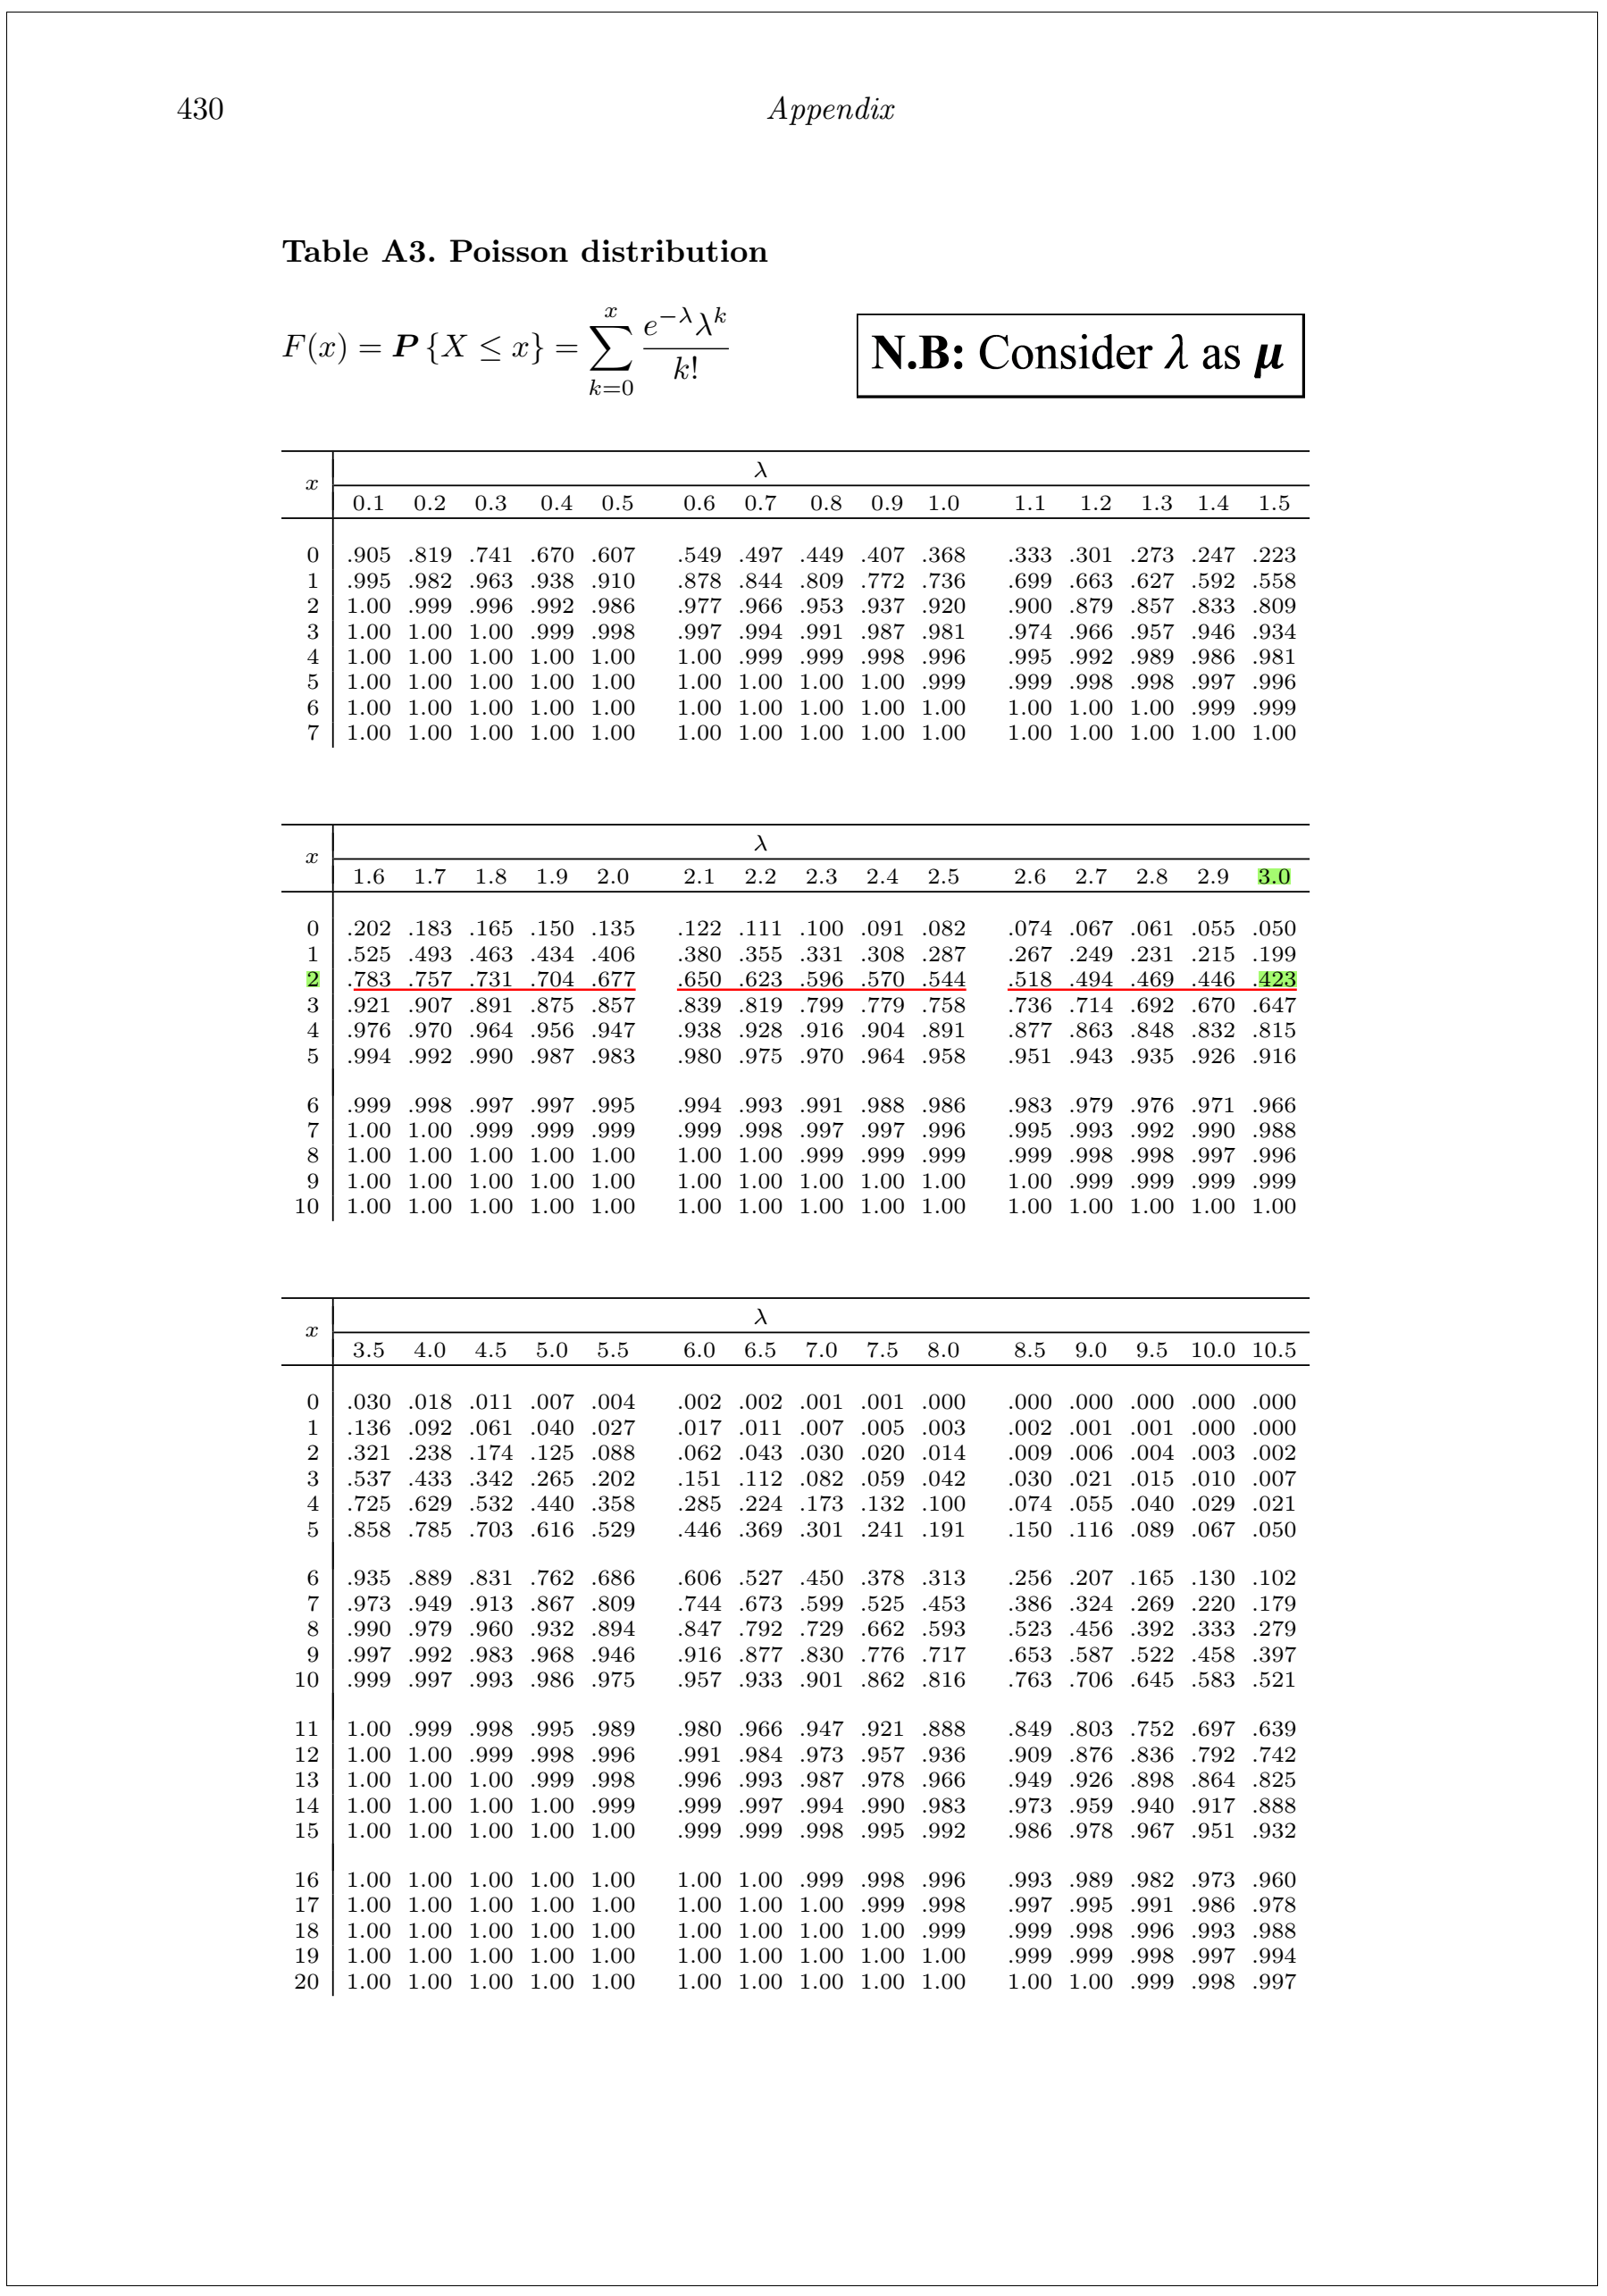
\includegraphics[keepaspectratio]{Poisson Table.png}}

\textbf{Consider} a discrete r.v say \(X\sim Pois(\lambda t)\). Suppose,
\(\lambda =1.5\) and \(t=2\). \textbf{Find}, (i) \(P(X \le 2)\)
(ii)P(X=4)

\textbf{\emph{Solution by using Table}}:

For \(t=2\) , \(\mu=\lambda t=1.5*2=3\).

\textbf{(i)} \(P(X \le 2)=F(2)=0.423\)

{[}For x=2 and \(\mu \ \ or \ \lambda =3\); corresponding probability in
\textbf{Table A3} is 0.423{]}

\textbf{(ii)} \(P(X=4)=f(4)=F(4)-F(3)=0.815-0.647=0.168\)

\textbf{Example 5.17:}(Walpole et al. 2017a) During a laboratory
experiment, the average number of radioactive particles passing through
a counter in 1 millisecond is 4. What is the probability that 6
particles enter the counter in a given millisecond?

\textbf{Example 5.18:}(Walpole et al. 2017a) Ten is the average number
of oil tankers arriving each day at a certain port. The facilities at
the port can handle at most 15 tankers per day. What is the probability
that on a given day tankers have to be turned away?

\textbf{Example 3.8:}{[}(Pishro-Nik 2014){]} The number of emails that I
get in a weekday can be modeled by a Poisson distribution with an
average of 0.2 emails per minute.

\begin{enumerate}
\def\labelenumi{\arabic{enumi}.}
\item
  What is the probability that I get no emails in an interval of length
  5 minutes?
\item
  What is the probability that I get more than 3 emails in an interval
  of length 10 minutes?
\end{enumerate}

\textbf{\emph{Solution}}

Let, \(X\)=number of emails that I get in a given interval.

Given, \(\lambda =0.2 \ \ min^{-1}\).

\(X\) will follow \(Pois(\lambda t)\)

\textbf{1.} In this case \(\mu=\lambda t=0.2*5=1\). \textbf{So},
\(P(X=0)=f(0)=e^{-\mu}=e^{-1}=0.3679\).

\textbf{2.} In this case \(\mu=\lambda t=0.2*10=2\).
\textbf{So},\(P(X>3)=1-P(X\le 3)=1-F(3)=1-0.857=0.143\). {[}From
\textbf{Table A3}{]}

\textbf{Approximation of Binomial Distribution to Poisson}

When,

\begin{itemize}
\item
  \(p \rightarrow0\) (\emph{Success rate is very low});
\item
  \(n\rightarrow \infty\) (\emph{Number of trials is very large});
\end{itemize}

Then \textbf{Binomial distribution} can be \emph{approximated} by
\textbf{Poisson distribution}.

\begin{itemize}
\tightlist
\item
  Mathematically, \(Binom (x; n,p)\approx Pois(\lambda)\); where
  \(\lambda=np\).
\end{itemize}

\textbf{N.B: In practical situation} if \(n \ge 30\) and \(p\le 0.05\)
;hence \(q\ge 0.95\),then the approximation is close enough to use the
Poisson distribution for binomial problems(Baron 2019).

\textbf{Example 5.20:}(Walpole et al. 2017a) In a manufacturing process
where glass products are made, defects or bubbles occur, occasionally
rendering the piece undesirable for marketing. It is known that, on
average, 1 in every 1000 of these items produced has one or more
bubbles. What is the probability that a random sample of 8000 will yield
fewer than 7 items possessing bubbles?

\textbf{\emph{Solution:}}

Let,\(X=number\ \ of \ \ glasses\ \ possesing\ \ bubbles\)

Given, \(Pr(buuble \ \ occurs)=p=1/1000=0.001\) which is less than
\(0.05\), and \(n=8000\) which is greater than \(30\). So, the PMF of
\(X\) can be approximated by Poisson distribution with

\[\lambda =np=8000*0.001=8\] that is \(X\sim Pois (\lambda=8)\)

According to question,

\(P(X<7)=f(0)+f(1)+...+f(6)=F(6)=0.313\) (\emph{Ans.})

{[}By using \textbf{Table A3}{]}

\textbf{Exercise 5.87:}(Walpole et al. 2017a) Imperfections in computer
circuit boards and computer chips lend themselves to statistical
treatment. For a particular type of board, the probability of a diode
failure is 0.03 and the board contains 200 diodes.

\begin{enumerate}
\def\labelenumi{(\alph{enumi})}
\item
  What is the mean number of failures among the diodes?
  (\textbf{\emph{Ans:}} \(\mu=np=200*0.03=6\))
\item
  What is the variance?(\textbf{\emph{Ans:}}
  \(\sigma^2=np(1-p)=200*0.03*(1-0.03)=5.82\))
\item
  The board will work if there are no defective diodes. What is the
  probability that a board will work? \textbf{\emph{Ans (c):}} The board
  will work if there are no defective diodes.

  So, P(The board will work)=\(P(X=0)=f(0)=e^{-\mu}=e^{-6}=0.0025\).
\end{enumerate}

\bookmarksetup{startatroot}

\chapter{Continuous r.v and probability density
function}\label{continuous-r.v-and-probability-density-function}

\section{\texorpdfstring{\textbf{Definition}}{Definition}}\label{definition}

A continuous r.v \(X\) must have a probability density function (PDF)
\(f(x)\) such that

1) \(f(x) \ge 0\) \textbf{{[}Non-negativity{]}}

2) \(\int_{x\in \mathbb{R}} f(x)dx =1\) \textbf{{[}Total AREA under the
curve} \(f(x)\) always 1{]}

3) \(P(a<X<b)=\int_a^b f(x) dx\)

\section{Illustration with an
example}\label{illustration-with-an-example}

Given \(f(x)=\frac{1}{2}x \ \ ; 0\le x\le 2\)

a) Show/plot the graph of \(f(x)\).

b) Is \(f(x)\) a PDF?

c) Find \(P(X<1.0)\).

d) Find \(P(X=1.0)\)

\textbf{\emph{Solution:}}

(a)

\begin{center}
\pandocbounded{
\includegraphics[keepaspectratio]{4Continuous_rv_5_files/figure-pdf/unnamed-chunk-1-1.pdf}}
\end{center}

b) Here, \(f(x)\ge 0\) for all values of \(x\) in the interval
\(0\le x\le2\).

Now, \textbf{total area under curve} \(f(x)\) from \(x=0\) to \(x=2\) is

\(\int_{0}^2 f(x)dx\)

\(=AREA \ \ of\ \  the\ \  SHADED\ \  Triangle\)

\begin{center}
\pandocbounded{
\includegraphics[keepaspectratio]{4Continuous_rv_5_files/figure-pdf/unnamed-chunk-2-1.pdf}}
\end{center}

\[=\frac{1}{2} \times base\times height\]

\[=\frac{1}{2} \times 2\times 1=1\]

So, total area under curve \(f(x)\) is \(1\) that is
\(\int_{0}^{2} f(x)dx=1\).

Hence, \(f(x)\) is a PDF.

c) Here,

\[P(X<1)=Area \ \ under\ \ the \ \ curve \ \ from \ \ x=0 \ \ to  \ \ x=1\]

\[=Area \ \ of \ \ the \ \ SHADED \ \ Triangle\]

\begin{center}
\pandocbounded{
\includegraphics[keepaspectratio]{4Continuous_rv_5_files/figure-pdf/unnamed-chunk-3-1.pdf}}
\end{center}

\[=\frac{1}{2}\times 1 \times f(1)=\frac{1}{2}\times 1 \times 0.5=0.25\]

Therefore \(P(X<1)=0.25\)

d) \(P(X=1.0)=0\) {[}Because there is no area at \(x=1.0\){]}

\begin{tcolorbox}[enhanced jigsaw, bottomrule=.15mm, toprule=.15mm, title=\textcolor{quarto-callout-note-color}{\faInfo}\hspace{0.5em}{Note}, bottomtitle=1mm, colframe=quarto-callout-note-color-frame, coltitle=black, rightrule=.15mm, toptitle=1mm, colbacktitle=quarto-callout-note-color!10!white, titlerule=0mm, breakable, arc=.35mm, leftrule=.75mm, opacitybacktitle=0.6, opacityback=0, colback=white, left=2mm]

We always remember that \textbf{Probability in an interval of} \(X\) is
a\textbf{ctually the} \(AREA\) \textbf{under the pdf} \(f(x)\)\textbf{.}

\end{tcolorbox}

\textbf{Problem 6.2.1} A random variable has the following density
function.

\[f(x)=1-0.5x \ \ ; \ \ 0<x<2\]\\
a) Graph the density function.

b) Verify that \(f(x)\) is a density function.

c) Fond \(P(X>1)\).

d) Find \(P(X<0.5)\).

e) Find \(P(X=1.5)\).

\textbf{N.B:} \(P(X=a)=0\) as well as \(P(X=b)=0\). So, \(P(X\le a )\)
is same as \(P(X<a)\).

\section{\texorpdfstring{\textbf{CDF of} continuous r.v
\(X\)}{CDF of continuous r.v X}}\label{cdf-of-continuous-r.v-x}

By definition, CDF,

\[F(x)=P(X\le x)= \int_{-\infty}^{x} f(x)dx\]

Therefore,

\begin{itemize}
\item
  \(f(x)=\frac{d}{dx} F(x)\).
\item
  \(P(a<X<b)=F(b)-F(a)\).
\end{itemize}

\section{\texorpdfstring{\textbf{Expectation and variance of continuous
r.v}}{Expectation and variance of continuous r.v}}\label{expectation-and-variance-of-continuous-r.v}

If \(X\) is a continuous r.v with PDF \(f(x)\) then

Expected value of \(X\) is

\[\mu=E(X)= \int_{x\in \mathbb{R}} x\cdot f(x)dx\] Variance of \(X\) is

\[Var(X)=E(X^2)-\mu^2=\int_{x\in \mathbb{R}} x^2\cdot f(x)dx-\mu^2\]

\textbf{Example 3.11}(Walpole et al. 2017a) Suppose that the error in
the reaction temperature, in \(^0C\), for a controlled laboratory
experiment is a continuous random variable X having the probability
density function

\[f(x)=\frac{x^2}{3}; -1<x<2.\]

\begin{enumerate}
\def\labelenumi{(\alph{enumi})}
\tightlist
\item
  Verify that \(f(x)\) is a density function.
\item
  Find \(P(0< X \le 1)\).
\end{enumerate}

\textbf{Example 3.12}(Walpole et al. 2017a) Find \(F(x)\), and use it to
evaluate \(P(0 < X\le1)\).

\textbf{H.W:} Find \(E(X)\) and \(Var(X)\)
where,\(f(x)=\frac{x^2}{3}; -1<x<2\).

\textbf{Exercise 3.29}(Walpole et al. 2017a) An important factor in
solid missile fuel is the particle size distribution. Significant
problems occur if the particle sizes are too large. From production data
in the past, it has been determined that the particle size (in
micrometers) distribution is characterized by

\[f(x)=3x^{-4}; x> 1\]

\begin{enumerate}
\def\labelenumi{(\alph{enumi})}
\tightlist
\item
  Verify that this is a valid density function.
\item
  Evaluate \(F(x)\).
\item
  What is the probability that a random particle from the manufactured
  fuel exceeds 4 micrometers?
\end{enumerate}

\textbf{Exercise 3.69}(Walpole et al. 2017a) The life span in hours of
an electrical component is a random variable with cumulative
distribution function

\[F(x)=1-e^{-\frac{x}{50}}; x>0\]

\begin{enumerate}
\def\labelenumi{(\alph{enumi})}
\item
  Determine its probability density function (PDF).
\item
  Determine the probability that the life span of such a component will
  exceed 70 hours.
\end{enumerate}

\textbf{Exercise 3.36} (Walpole et al. 2017a) On a laboratory
assignment, if the equipment is working, the density function of the
observed outcome, \(X\), is

\[f(x)=2(1-x) \ \ ; 0<x<1\]

\begin{enumerate}
\def\labelenumi{\alph{enumi}.}
\item
  Calculate \(P(X\le 1)\)
\item
  What is the probability that \(X\) will exceed 0.5?
\item
  Given that \(X \ge 0.5\), what is the probability that \(X\) will be
  less than 0.75?
\end{enumerate}

\textbf{Hints:} We can solve this exercise by either using \(F(x)\) or
simply drawing function \(f(x)\).

\section{Uniform distribution/r.v}\label{uniform-distributionr.v}

A continuous r.v \(X\) is said to be uniform r.v ranges between \(a\) to
\(b\) if it has the following PDF

\[f(x)=\frac{1}{b-a} \ \ ; \ \ a<x<b\] \{\#eq-unif.pdf\}

\begin{figure}

\centering{

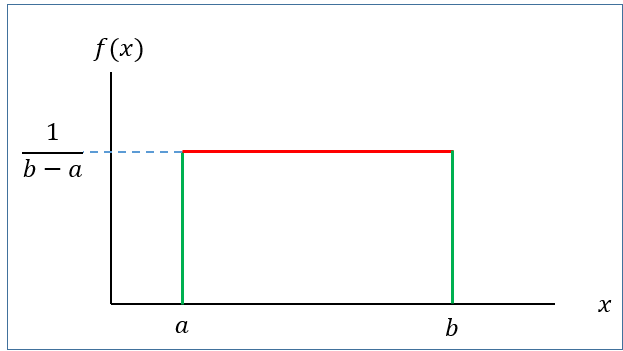
\includegraphics[width=3.92708in,height=\textheight,keepaspectratio]{images/clipboard-3046233387.png}

}

\caption{\label{fig-unifpdf}Graph of f(x)}

\end{figure}%

with

\textbf{Mean:} \(\mu=E(X)=\frac{a+b}{2}\)

\textbf{Variance:} \(\sigma^2=\frac{(b-a)^2}{12}\)

\ul{\textbf{We write,}} \(X\sim U(a,b)\)

\subsection{Finding probability for uniform
r.v}\label{finding-probability-for-uniform-r.v}

If \(X\sim U(a,b)\) then the \(P(x_1<X<x_2)\) is actually the
\textbf{area of the shaded rectangle.}

\begin{figure}[H]

{\centering 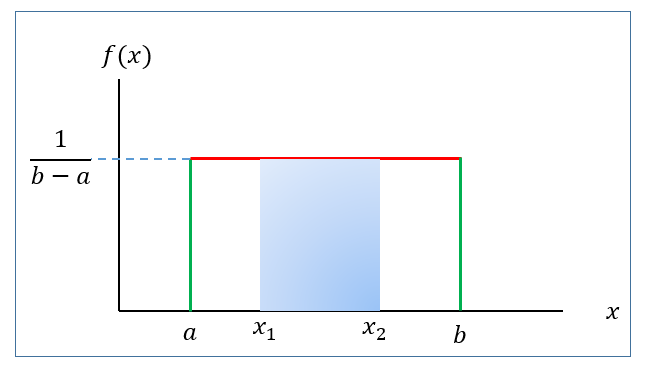
\includegraphics[width=3.95833in,height=\textheight,keepaspectratio]{images/clipboard-2570030964.png}

}

\caption{Computing area for an interval of Uniform distribution}

\end{figure}%

That is,

\[P(x_1<X<x_2)=Base\times Height=(x_2-x_1)\times \frac{1}{b-a}\]

\textbf{Problem 1} The phase angle, \(\Theta\), of the signal at the
input to a modem is uniformly distributed between \(0\) and \(2\pi\)
radians.

a) What are the PDF, expected value, and variance of \(\Theta\)?

b) Find the probability that phase angle exceeds \(\frac{3\pi}{2}\)?

\textbf{Problem 2} In a radio communications system, the phase
difference \(X\) between the transmitter and receiver is modeled as
having a uniform density in \([—\pi, +\pi]\). Find \(P(X < 0)\) and
\(P(X< \pi/2)\).\\

\textbf{Problem} \textbf{3}(Navidi 2011, 278) Resistors are labeled 100
\(\Omega\). In fact, the actual resistances are uniformly distributed on
the interval \((95, 103)\).

a. Find the mean resistance.

b. Find the standard deviation of the resistances.

c. Find the probability that the resistance is between \(98\) and
\(102 \ \ \Omega\).

d. Suppose that resistances of different resistors are independent. What
is the probability that three out of six resistors have resistances
greater than \(100\) \(\Omega\)?

\subsection{Generating Uniform random number in
R}\label{generating-uniform-random-number-in-r}

\begin{Shaded}
\begin{Highlighting}[]
\FunctionTok{par}\NormalTok{(}\AttributeTok{mar=}\FunctionTok{c}\NormalTok{(}\DecValTok{4}\NormalTok{,}\DecValTok{4}\NormalTok{,}\DecValTok{1}\NormalTok{,}\DecValTok{1}\NormalTok{)) }\CommentTok{\# Adjust graph margin}
\FunctionTok{set.seed}\NormalTok{(}\DecValTok{911}\NormalTok{) }
\NormalTok{u}\OtherTok{=}\FunctionTok{runif}\NormalTok{(}\DecValTok{1000}\NormalTok{,}\DecValTok{10}\NormalTok{,}\DecValTok{30}\NormalTok{) }\CommentTok{\# Generating 1000 random numbers from U(10,30)}
\FunctionTok{hist}\NormalTok{(u,}\AttributeTok{main =} \StringTok{" "}\NormalTok{,}\AttributeTok{col=}\StringTok{"steelblue"}\NormalTok{,}\AttributeTok{ylim =} \FunctionTok{c}\NormalTok{(}\DecValTok{0}\NormalTok{,}\DecValTok{120}\NormalTok{)) }\CommentTok{\# Frequency histogram of U}
\end{Highlighting}
\end{Shaded}

\begin{figure}[H]

\pandocbounded{
\includegraphics[keepaspectratio]{4Continuous_rv_5_files/figure-pdf/fig-unifhist-1.pdf}}

\caption{\label{fig-unifhist}Histogram of Uniform random numbers from
U(10,30), \(\ n=1000\)}

\end{figure}%

\section{Normal or Gaussian r.v}\label{normal-or-gaussian-r.v}

The most important probability distribution for describing a continuous
random variable is the \textbf{normal probability distribution}. The
normal distribution has been used in a wide variety of practical
applications in which the random variables are heights and weights of
people, test scores, scientific measurements, amounts of rainfall, and
other similar values.

\subsection{Definition}\label{definition-1}

A continuous r.v \(X\) is said to be normal r.v if it has the following
\textbf{PDF:}

\[f(x)=\frac{1}{\sigma \sqrt{2\pi}} e^{-\frac{1}{2} (\frac{x-\mu}{\sigma})^2}\ \ ; -\infty<x<\infty\]
\{\#eq-normal\}

The graph of \(f(x)\) is called \textbf{normal curve}
(Figure~\ref{fig-normalpdf})\textbf{.}

\begin{figure}

\pandocbounded{
\includegraphics[keepaspectratio]{4Continuous_rv_5_files/figure-pdf/fig-normalpdf-1.pdf}}

\caption{\label{fig-normalpdf}Normal Curve}

\end{figure}%

\textbf{Mean:} \(E(X)=\mu\)

\textbf{Variance:} \(Var(X)=\sigma^2\)

\ul{\textbf{We write:}} \(X\sim N(\mu , \sigma^2)\)

\textbf{Properties of normal distribution}

\begin{itemize}
\item
  The \textbf{total area} under the normal curve \(f(x)\) is 1 that is

  \[\int_{-\infty}^{\infty} f(x)dx=1\]
\item
  Normal distribution is symmetric about mean, \(\mu\)
\item
  Mean, median and mode is identical in normal distribution that is
  \(Mean=Median=Mode=\mu\)
\item
  Almost \(99\%\) observations of \(X\) lie within \textbf{3 standard
  deviation of mean} that is

  \[P(\mu-3\sigma<X<\mu+3\sigma)\approx 0.99\]
\item
  Almost \(95\%\) observations of \(X\) lie within \textbf{2 standard
  deviation of mean} that is
  \[P(\mu-2\sigma<X<\mu+2\sigma)\approx 0.95\]
\item
  Almost \(68\%\) observations of \(X\) lie within \textbf{1 standard
  deviation of mean} that is \[P(\mu-\sigma<X<\mu+\sigma)\approx 0.68\]
\end{itemize}

\subsection{Standard normal r.v}\label{standard-normal-r.v}

Suppose \(X\sim N(\mu, \sigma^2)\). Then the variable
\(Z=\frac{X-\mu}{\sigma}\) is said to be \textbf{standard normal
variable} with \textbf{PDF}

\[f(z)=\frac{1}{\sqrt {2\pi}} e^{-z^2} \ \ ; -\infty<z<\infty\]
\{\#eq-standardnorm\}

\textbf{Mean:} \(E(Z)=0\)

\textbf{Variance:} \(Var(Z)=1\)

\ul{\textbf{We write:}} \(Z\sim N(0,1)\)

\begin{figure}

\pandocbounded{
\includegraphics[keepaspectratio]{4Continuous_rv_5_files/figure-pdf/fig-zcurve-1.pdf}}

\caption{\label{fig-zcurve}Standard normal curve}

\end{figure}%

\subsection{Computing probability(area) under standard normal
curve}\label{computing-probabilityarea-under-standard-normal-curve}

To compute area (probability) under the standard normal curve for a
given interval of \(z\) we use \textbf{standard Normal Distribution}
\textbf{table} which provides cumulative probabilities.

\textbf{RULE-I:} Suppose we want to find \(P(Z<1.25)\).

From \textbf{TABLE A.2} in Navidi (2011) we have

\[P(Z<1.25)=0.8944\]

\pandocbounded{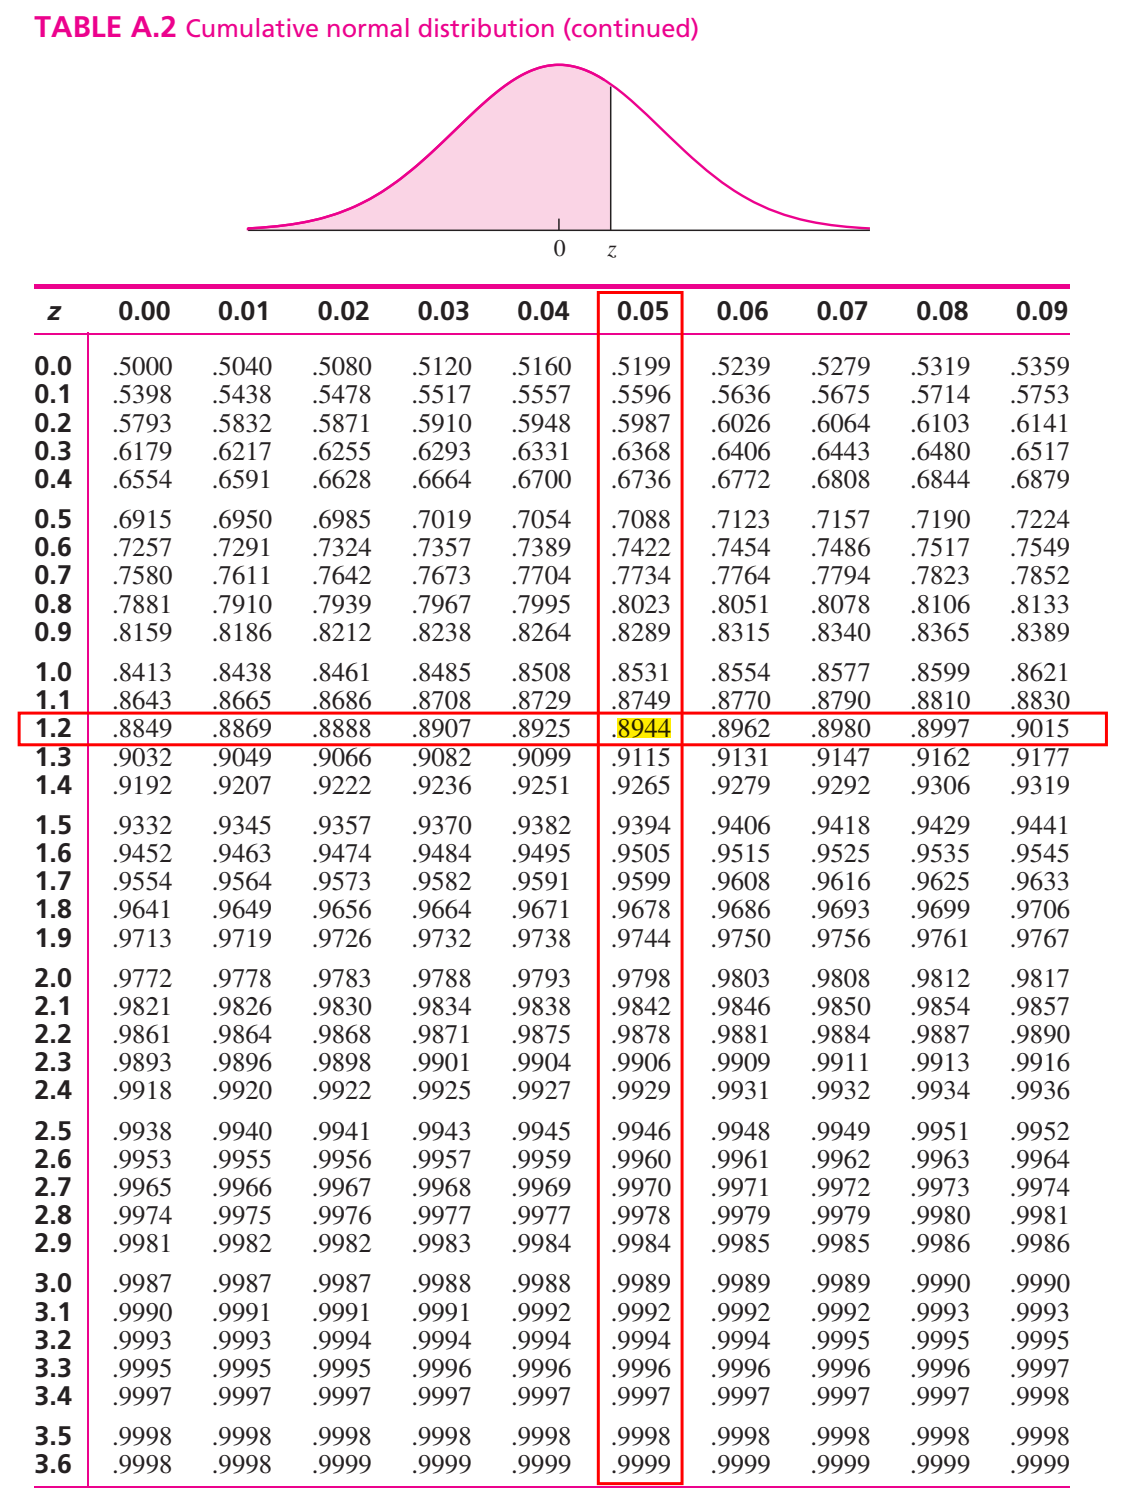
\includegraphics[keepaspectratio]{images/clipboard-386943420.png}}\\
The probability \(P(Z<1.25)\) is shown in Figure~\ref{fig-areaz}.

\begin{figure}

\pandocbounded{
\includegraphics[keepaspectratio]{4Continuous_rv_5_files/figure-pdf/fig-areaz-1.pdf}}

\caption{\label{fig-areaz}Area under standard normal curve for
Z\textless1.25}

\end{figure}%

\textbf{RULE-II:} Now we find \(P(Z>1.36)\)

So, due to symmetry we can write \(P(Z>1.36)=P(Z<-1.36)=0.0869\)\\

\begin{figure}

\pandocbounded{
\includegraphics[keepaspectratio]{4Continuous_rv_5_files/figure-pdf/fig-areaz2-1.pdf}}

\caption{\label{fig-areaz2}Area under standard normal curve for
Z\textgreater1.36}

\end{figure}%

\textbf{RULE-III:} Let us evaluate \(P(-1.96<Z<2.58)\).

We can write

\[=P(-1.96<Z<2.58)\]

\[=P(Z<2.58)-P(Z<-1.96)\]

\[=0.9951-0.0250=0.9701\]

\begin{figure}

\pandocbounded{
\includegraphics[keepaspectratio]{4Continuous_rv_5_files/figure-pdf/fig-areaz3-1.pdf}}

\caption{\label{fig-areaz3}Area under standard normal curve for
-1.96\textless Z\textless2.58}

\end{figure}%

\subsection{\texorpdfstring{Finding quantiles (percentiles, quartiles,
deciles etc.) of
\(Z\)}{Finding quantiles (percentiles, quartiles, deciles etc.) of Z}}\label{finding-quantiles-percentiles-quartiles-deciles-etc.-of-z}

What is the \(90^{th}\) percentile of \(Z\)? To answer this question,
let \(k\) is the \(90^{th}\) percentile of \(Z\). So we can write

\[P(Z<k)=0.90 \ \  \ \ \ \ \ \ \ \cdot \cdot \cdot (1)\]

From \textbf{TABLE A.2} in Navidi (2011) we have

\[P(Z<1.28)=0.90 \ \  \ \ \ \ \ \ \ \cdot \cdot \cdot(2)\]

Comparing eq.(1) with eq.(2) we have \(k=1.28\). So the \(90^{th}\)
percentile of \(Z\) is \(1.28\).

\textbf{Problem 1} Find \(c\) such that \(P(Z>c)=0.05\).

\textbf{Problem 2} Find \(c\) such that \(P(-c<Z<c)=0.95\).

\subsection{Computing probability(area) under normal
curve:}\label{computing-probabilityarea-under-normal-curve}

Suppose \(X\sim N(30, 5^2)\) . Then find the following:

a) \(P(X<22)\)

b) \(P(X>44)\)

c) \(P(20<X<35)\)

d) If \(P(X<x)=0.25\) then find the value of \(x\).

\textbf{\emph{Solution:}}

Here, \(\mu=30\) and \(\sigma=5\)

\begin{center}\rule{0.5\linewidth}{0.5pt}\end{center}

a)
\(P(X<22)=P(\frac{X-\mu}{\sigma}<\frac{22-30}{5})=P(Z<-1.60)=0.0548\).

\begin{center}\rule{0.5\linewidth}{0.5pt}\end{center}

b) \(P(X>44)=P(\frac{X-\mu}{\sigma}>\frac{44-30}{5})\)

\(=P(Z>2.80)=P(Z<-2.80)=0.0026\)

\begin{center}\rule{0.5\linewidth}{0.5pt}\end{center}

c)
\(P(20<X<35)=P(\frac{20-30}{5}<\frac{X-\mu}{\sigma}<\frac{35-30}{5})\)

\(=P(-2<Z<1)=P(Z<1)-P(Z<-2)\)

\(=0.8413-0.0228=0.8185\)

\begin{center}\rule{0.5\linewidth}{0.5pt}\end{center}

d) To find the value of \(x\) we proceed this way.

\[P(X<x)=0.25\]

\[\implies P(\frac{X-\mu}{\sigma}<\frac{x-30}{5})=0.25\]

\[\implies P(Z<\frac{x-30}{5})=0.25 \ \ \ \ \ \cdot \cdot \cdot (1)\]

From TABLE (Appendix B) we have

\[P(Z<-0.67)=0.25  \ \ \ \ \cdot \cdot \cdot (2)\]

Comparing (1) with (2) we can write

\[\frac{x-30}{5}=-0.67\]

\[\implies x=30+(-0.67)\times 5\]

\[\therefore x=26.65\]

\begin{tcolorbox}[enhanced jigsaw, bottomrule=.15mm, toprule=.15mm, title=\textcolor{quarto-callout-note-color}{\faInfo}\hspace{0.5em}{Note}, bottomtitle=1mm, colframe=quarto-callout-note-color-frame, coltitle=black, rightrule=.15mm, toptitle=1mm, colbacktitle=quarto-callout-note-color!10!white, titlerule=0mm, breakable, arc=.35mm, leftrule=.75mm, opacitybacktitle=0.6, opacityback=0, colback=white, left=2mm]

If \(P(X<x)=p\) and

\(P(Z<z)=p\) then

\[x=\mu+z\sigma\]

\end{tcolorbox}

\subsection{Applications of the Normal Distribution (Walpole et al.
2017a)}\label{applications-of-the-normal-distribution-walpole2017}

\textbf{Example 6.7}: A certain type of storage battery lasts, on
average, 3.0 years with a standard deviation of 0.5 year. Assuming that
battery life is normally distributed, find the probability that a given
battery will last less than 2.3 years.

\textbf{Example 6.8} : An electrical firm manufactures light bulbs that
have a life, before burn-out, that is normally distributed with mean
equal to 800 hours and a standard deviation of 40 hours. Find the
probability that a bulb burns between 778 and 834 hours.

\textbf{Example 6.9} : In an industrial process, the diameter of a ball
bearing is an important measurement. The buyer sets specifications for
the diameter to be \(3.0 \pm 0.01\) cm. The implication is that no part
falling outside these specifications will be accepted. It is known that
in the process the diameter of a ball bearing has a normal distribution
with mean \(\mu = 3.0\) and standard deviation \(\sigma = 0.005\). On
average, how many manufactured ball bearings will be scrapped?

\textbf{Example 6.10} : Gauges are used to reject all components for
which a certain dimension is not within the specification
\(1.50 \pm d\). It is known that this measurement is normally
distributed with a mean of 1.50 and a standard deviation of 0.2.
Determine the value d such that the specifications ``cover'' 95\% of the
measurements.

\textbf{Solution:}

Let, \(X=measurement \ \ of \ \ certain \ \ dimension\)

Given, \(X\sim N(1.5,0.2)\)

According to question,

\(P(1.5-d<X<1.5+d)=0.95\)

So, \(P(X<1.5-d)+P(X>1.5+d)=0.05\)

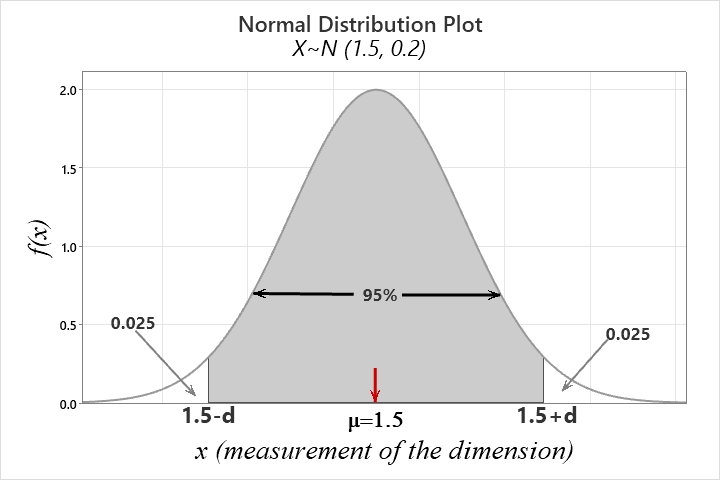
\includegraphics[width=4.20833in,height=2.48958in]{images/clipboard-1813690955.png}

So, \(P(X <1.5-d)=0.025  \ \ \ \ \cdot \cdot \cdot(1)\)

\(\implies P(\frac{X-\mu}{\sigma} <\frac{1.5-d-1.5}{0.2})=0.025\)

\(\implies P(Z<\frac{-d}{0.2})=0.025 \ \ \ \ \cdot \cdot \cdot(1)\)

From TABLE A.2 we have

\(P(Z<-1.96)=0.025 \ \ \ \ \ \cdot \cdot\cdot(2)\)

Comparing eq.(1) with eq. (2) we have

\(\frac{-d}{0.2}=-1.96\)

\(\implies -d=-0.392\)

\(\therefore d=0.392\)

\textbf{Alternative:}

\(P(X <1.5-d)=0.025  \ \ \ \ \cdot \cdot \cdot(1)\)

But, \(P(Z<-1.96)=0.025 \ \ \ \ \cdot \cdot \cdot (2)\)

Hence, \(1.5-d=\mu+z\sigma\); where \(z=-1.96\)

\(\implies 1.5-d=1.5-1.96\times 0.2\)

\(\therefore d=0.392\)

\textbf{Exercise 6.11} : A soft-drink machine is regulated so that it
discharges an average of 200 milliliters per cup. If the amount of drink
is normally distributed with a standard deviation equal to 15
milliliters,

\begin{enumerate}
\def\labelenumi{(\alph{enumi})}
\tightlist
\item
  what fraction of the cups will contain more than 224 milliliters?
\item
  what is the probability that a cup contains between 191 and 209
  milliliters?
\item
  how many cups will probably overflow if 230-milliliter cups are used
  for the next 1000 drinks?
\item
  below what value do we get the smallest 25\% of the drinks?
\end{enumerate}

\textbf{Exercise 6.14} The finished inside diameter of a piston ring is
normally distributed with a mean of 10 centimeters and a standard
deviation of 0.03 centimeter.

\begin{enumerate}
\def\labelenumi{(\alph{enumi})}
\tightlist
\item
  What proportion of rings will have inside diameters exceeding 10.075
  centimeters?
\item
  What is the probability that a piston ring will have an inside
  diameter between 9.97 and 10.03 centimeters?
\item
  Below what value of inside diameter will 15\% of the piston rings
  fall?
\end{enumerate}

\textbf{Exercise 6.17} : The average life of a certain type of small
motor is 10 years with a standard deviation of 2 years. The manufacturer
replaces free all motors that fail while under guarantee. If she is
willing to replace only 3\% of the motors that fail, how long a
guarantee should be offered? Assume that the lifetime of a motor follows
a normal distribution.

\subsection{Normal approximation to Binomial
distribution}\label{normal-approximation-to-binomial-distribution}

Binom tends to normal when \(n \rightarrow \infty\) and
\(p\rightarrow 0.5\)

\begin{figure}

\pandocbounded{
\includegraphics[keepaspectratio]{4Continuous_rv_5_files/figure-pdf/fig-bintonorm1-1.pdf}}

\caption{\label{fig-bintonorm1}Histogram of \(Bin(x; n=6,p=0.2)\)}

\end{figure}%

\begin{figure}

\pandocbounded{
\includegraphics[keepaspectratio]{4Continuous_rv_5_files/figure-pdf/fig-bintonorm2-1.pdf}}

\caption{\label{fig-bintonorm2}Histogram of \(Bin(x; n=15,p=0.2)\)}

\end{figure}%

\begin{figure}

\pandocbounded{
\includegraphics[keepaspectratio]{4Continuous_rv_5_files/figure-pdf/fig-bintonorm3-1.pdf}}

\caption{\label{fig-bintonorm3}Histogram of \(Bin(x; n=50,p=0.2)\)}

\end{figure}%

From Figure~\ref{fig-bintonorm1}, Figure~\ref{fig-bintonorm2} and
Figure~\ref{fig-bintonorm3} we observe that as \(n\) getting large with
\(p=0.2\) (which is not extremely close to 0) the binomial distribution
can be approximated to normal distribution.

So, when \(n\) become large and \(p\) is not extremely small (close to
0) or extremely large (close to 1) the normal approximation is most
useful in calculating binomial sums.

\begin{tcolorbox}[enhanced jigsaw, bottomrule=.15mm, toprule=.15mm, title=\textcolor{quarto-callout-important-color}{\faExclamation}\hspace{0.5em}{Normal Approximation to the Binomial Distribution}, bottomtitle=1mm, colframe=quarto-callout-important-color-frame, coltitle=black, rightrule=.15mm, toptitle=1mm, colbacktitle=quarto-callout-important-color!10!white, titlerule=0mm, breakable, arc=.35mm, leftrule=.75mm, opacitybacktitle=0.6, opacityback=0, colback=white, left=2mm]

\begin{itemize}
\item
  Let X be a binomial random variable with parameters \(n\) and \(p\).
  For large \(n\), \(X\) has approximately a normal distribution with
  \(\mu = np\) and \(\sigma^2 =np(1-p)\).
\item
  The approximation will be good if \(np\) and \(n(1-p)\) are greater
  than or equal to \(5\) (Walpole et al. 2017a).
\end{itemize}

\end{tcolorbox}

\textbf{Continuity correction}

This correction is needed when we approximate a discrete distribution
(Binomial in this case) by a continuous distribution (Normal). Recall
that the probability \(P(X = x)\) may be positive if \(X\) is discrete,
whereas it is always \(0\) for continuous \(X\). This is resolved by
introducing a continuity correction. Expand the interval by 0.5 units in
each direction, then use the Normal approximation (Baron 2019).

\begin{longtable}[]{@{}cc@{}}
\caption{Continuity correction for binomial
probabilities}\tabularnewline
\toprule\noalign{}
Binomial Probability & With continuity correction \\
\midrule\noalign{}
\endfirsthead
\toprule\noalign{}
Binomial Probability & With continuity correction \\
\midrule\noalign{}
\endhead
\bottomrule\noalign{}
\endlastfoot
\(P(X=x)\) & \(P(x-0.5<X<x+0.5)\) \\
\(P(X\le x)\) & \(P(X\le x+0.5)\) \\
\end{longtable}

\textbf{Example 6.15} (Walpole et al. 2017a, 191): The probability that
a patient recovers from a rare blood disease is 0.4. If 100 people are
known to have contracted this disease, what is the probability that
fewer than 30 survive?

\section{Exponential r.v}\label{exponential-r.v}

In many situations, such as when modeling waiting times, inter-arrival
times, the lifespan of hardware, breakdown times, and the intervals
between phone calls, the exponential distribution is utilized. The time
(suppose \(T\)) between rare events in Poisson process with arrival rate
\(\lambda\) (\emph{number of arrival per unit time}) can be treated as
exponential r.v.

The exponential r.v \(T\) has the following PDF

\[f(t)=\lambda e^{-\lambda t} \ \ ; \ \ t>0\] \{\#eq-expo\}

\begin{itemize}
\item
  \textbf{CDF:} \(F(t)=P(T\le t)=P(T< t)=1-e^{-\lambda t}; t> 0\)

  Hence, \(P(T> t)=1-P(T\le t)=1-F(t)=e^{-\lambda t}\)
\item
  \textbf{Mean:} \(E(T)=\frac{1}{\lambda}\)
\item
  \textbf{Variance:} \(Var(T)=\frac{1}{\lambda^2}\)
\item
  \ul{\textbf{We write}}\textbf{,} \(T\sim Exp(\lambda)\)
\end{itemize}

\begin{figure}

\centering{

\pandocbounded{
\includegraphics[keepaspectratio]{4Continuous_rv_5_files/figure-pdf/fig-expo-1.pdf}}

}

\caption{\label{fig-expo}Exponential probability density functions for
selected values of \(\lambda\)}

\end{figure}%

The quantity \(\lambda\) is a parameter of Exponential distribution, and
its meaning is clear from \(E(T) = \frac{1}{\lambda}\) . If T is time,
measured in minutes, then \(\lambda\) is a frequency, measured in
\(min^{-1}\). For example, if arrivals occur every half a minute, on the
average, then \(E(T) = 0.5\)min and \(\lambda=2\), saying that they
occur with a frequency (arrival rate) of 2 arrivals per minute. This
\(\lambda\) has the same meaning as the parameter of Poisson
distribution(Baron 2019).

\textbf{Example 4.5}(Baron 2019) Jobs are sent to a printer at an
average rate of 3 jobs per hour.

\begin{enumerate}
\def\labelenumi{(\alph{enumi})}
\item
  What is the expected time between jobs?
\item
  What is the probability that the next job is sent within 5 minutes?
\end{enumerate}

\textbf{Solution:} Given, number of jobs per hour,
\(\lambda=3\ \ hr^{-1}\) per hour. Let, \(T\)=time elapsed between jobs
(hour).

So, \(T\sim Exp(\lambda)\)

\begin{enumerate}
\def\labelenumi{(\alph{enumi})}
\item
  \(E(T)=\frac{1}{\lambda} hr=\frac{1}{3} hr=20\ \ mins\);
\item
  Here, \(5 \ \ mins=\frac{5}{60} hr=\frac{1}{12} hr\) We know,
  \(F(t)=1-e^{-\lambda t}; t>0\)
\end{enumerate}

So,
\(P(T<5 \ \ mins)=P(T<\frac{1}{12})=F(\frac{1}{12})=1-e^{-3*\frac{1}{12}}=0.22\)

\textbf{Example 4.58} (Navidi 2011) A radioactive mass emits particles
according to a Poisson process at a mean rate of 15 particles per
minute. At some point, a clock is started. What is the probability that
more than 5 seconds will elapse before the next emission? What is the
mean waiting time until the next particle is emitted?

\textbf{Solution}

Let,
\(T=elapsed \ \ time \ \ before \ \ the \ \ next \ \ emission (in \ \ second)\)

Given, \(\lambda=15 min^{-1}=\frac{15}{60} s^{-1}=0.25 s^{-1}\) and

\(T\sim Exp(\lambda)\);

\(P(T\le t)=F(t)=1-e^{-\lambda t}\)

\emph{P(more than 5 seconds will elapse before the next
emission)}=\(P(T>5)=e^{-\lambda * 5}=e^{-0.25*5}=0.2865\)

\emph{Mean waiting time},
\(E(T)=\frac{1}{\lambda} s=\frac{1}{0.25}s=4s\)

\subsection{Lack of Memory Property}\label{lack-of-memory-property}

If \(T \sim Exp(\lambda)\), and \(t\) and \(s\) are positive numbers,
then

\[P(T> t+s| T> s)=P(T> t)\]

We can also express the \emph{Lack of memory property} in this way:

\[P(T< t+s| T> s)=P(T< t)\]

The probability that we must wait additional \(t\) units, given that we
have already waited \(s\) units, is the same as the probability that we
must wait \(t\) units from the start. The exponential distribution does
not ``\emph{remember}'' how long we have been waiting.

\begin{itemize}
\item
  In particular, if the lifetime of a component follows the exponential
  distribution, then the probability that a component that is \(s\) time
  units old will last an additional \(t\) time units is the same as the
  probability that a new component will last \(t\) time units.
\item
  In other words, a component whose lifetime follows an exponential
  distribution does not show any effects of age or wear(Navidi 2011).
\item
  But if the failure of the component is a result of gradual or slow
  wear (as in mechanical wear), then the exponential does not apply and
  either the \textbf{gamma} or the \textbf{Weibull distribution} (see
  (Walpole et al. 2017a), Section 6.10) may be more appropriate.
\end{itemize}

\textbf{Example 4.59}(Navidi 2011) The lifetime of a particular
integrated circuit has an exponential distribution with mean 2 years.
Find the probability that the circuit lasts longer than three years.

\textbf{Example 4.60}(Navidi 2011) Refer to Example 4.59. Assume the
circuit is now four years old and is still functioning. Find the
probability that it functions for more than three additional years
(Hints: Apply Lack of Memory Property).

\textbf{Exercises for Section 4.7}(Navidi 2011)

1.Let \(T \sim Exp(0.45)\). Find \(\mu_T, \sigma^2_T, P(T>3)\) and the
median of \(T\).

2.The time between requests to a web server is exponentially distributed
with mean 0.5 seconds.

\begin{enumerate}
\def\labelenumi{\alph{enumi}.}
\tightlist
\item
  What is the value of the parameter \(\lambda\)?
\item
  What is the median time between requests?
\item
  What is the standard deviation?
\item
  What is the 80th percentile?
\item
  Find the probability that more than one second elapses between
  requests.
\item
  If there have been no requests for the past two seconds, what is the
  probability that there more than one additional second will elapse
  before the next request?
\end{enumerate}

\textbf{\emph{Solution}}

Let, \(T=time \ \ between \ \ requests \ \ in \ \ second\)

If, \(T\sim Exp(\lambda)\); then it is given that

\(E(T)=0.5 \ \ second\)

\(\implies \frac{1}{\lambda}=0.5 \ \ second\)

\textbf{a.} \(\therefore \lambda=2 s^{-1}\)

\textbf{b.} If \(M\) is the median time between request then,

\(P(T \le M)=0.5\)

\(\implies F(M)=0.5\)

\(\implies 1-e^{-\lambda *M}=0.5\)

\(\implies e^{-\lambda *M}=0.5\)

\(\implies {-\lambda *M}=ln(0.5)\)

\(\implies M =\frac{ln(0.5)}{-\lambda}=\frac{ln(0.5)}{-2}=0.3466\approx0.35\)

So, median time between request is \(0.35s\)

\textbf{c.} Standard deviation of \(T\),
\(\sigma_T=\frac{1}{\lambda}s=1/2 =0.5 s\)

\textbf{d.} Let, \(P_{80}\) denotes 80th percentile.

So, solve the following equation for \(P_{80}\)

\(P(T\le P_{80})=0.80\)

\(\implies P(T>P_{80})=0.20\)

\(\implies e^{-\lambda \times P_{80}}=0.20\)

\(\implies P_{80}=\frac {ln(0.20)}{-\lambda}=0.805\)

\(\therefore P_{80}=0.805 s\)

\textbf{e.} \(P(T>1)=e^{-\lambda *1}=0.1353\)

\textbf{f.} If there have been no requests for the past two seconds, the
probability that there more than \textbf{\emph{one}} \textbf{additional
second} will elapse before the next request is:

\(P(T>1+2 /T>2)=P(T>1)=e^{-\lambda *1}=0.1353\) {[}by using \emph{Lack
of memory property}{]}

8.A radioactive mass emits particles according to a Poisson process at a
mean rate of 2 per second. Let T be the waiting time, in seconds,
between emissions.

\begin{enumerate}
\def\labelenumi{\alph{enumi}.}
\tightlist
\item
  What is the mean waiting time?
\item
  What is the median waiting time?
\item
  Find \(P(T > 2)\). Hint:\(P(T > 2)=e^{-\lambda *2}\)
\item
  Find \(P(T < 0.1)\).Hint:\(P(T < 0.1)=F(0.1)\)
\item
  Find \(P(0.3< T < 1.5)\). Hint:\(P(0.3< T < 1.5)=F(1.5)-F(0.3)\)
\item
  If 3 seconds have elapsed with no emission, what is the probability
  that there will be an emission within the next second? (Use Lack of
  Memory Property)
\end{enumerate}

\textbf{Solution of f.}

Since T is exponentially distributed and hold lack of memory property,
so it dose not matter what was happened in past 3 seconds. We have to
just compute that \emph{there will be an emission (event will occur)
within the next second}. So,

\(P(T<1)=F(1)=1-e^{-\lambda*1}\) (\emph{do yourself})

\subsection{Generating exponential random numbers in
R}\label{generating-exponential-random-numbers-in-r}

\begin{Shaded}
\begin{Highlighting}[]
\FunctionTok{par}\NormalTok{(}\AttributeTok{mar=}\FunctionTok{c}\NormalTok{(}\DecValTok{4}\NormalTok{,}\DecValTok{4}\NormalTok{,}\DecValTok{1}\NormalTok{,}\DecValTok{1}\NormalTok{)) }\CommentTok{\# Adjust graph margin}
\FunctionTok{set.seed}\NormalTok{(}\DecValTok{911}\NormalTok{) }
\NormalTok{t}\OtherTok{=}\FunctionTok{rexp}\NormalTok{(}\DecValTok{1000}\NormalTok{,}\AttributeTok{rate =} \FloatTok{2.5}\NormalTok{)}
\FunctionTok{hist}\NormalTok{(t, }\AttributeTok{main =} \StringTok{""}\NormalTok{,}\AttributeTok{col =} \StringTok{"steelblue"}\NormalTok{)}
\end{Highlighting}
\end{Shaded}

\begin{figure}[H]

\pandocbounded{
\includegraphics[keepaspectratio]{4Continuous_rv_5_files/figure-pdf/fig-rexpo-1.pdf}}

\caption{\label{fig-rexpo}Histogram of exponential random variable from
Exp(\(\lambda=2.5)\),\(\ n=1000\)}

\end{figure}%

\bookmarksetup{startatroot}

\chapter{Joint Probability
Distributions}\label{joint-probability-distributions}

\section{Joint PMF}\label{joint-pmf}

\section{Joint PDF}\label{joint-pdf}

\section{Marginal Prob. Dist.}\label{marginal-prob.-dist.}

\section{Conditional Prob. Dist.}\label{conditional-prob.-dist.}

\section{Stochastic Independence}\label{stochastic-independence}

\section{Covariance and Correlation}\label{covariance-and-correlation}

\section{Common Joint Probability
Distributions}\label{common-joint-probability-distributions}

\subsection{Multinomial}\label{multinomial}

\subsection{Bivariate Normal}\label{bivariate-normal}

\section{Linear Functions of Random
Variables}\label{linear-functions-of-random-variables}

\subsection{Transformations}\label{transformations}

\section{Moment Generating Functions}\label{moment-generating-functions}

\bookmarksetup{startatroot}

\chapter{Statistical inference}\label{statistical-inference}

\textbf{Statistical inference} refers to the branch of statistics that
focuses on making decisions and drawing conclusions about populations
based on sample data. These methods use information collected from a
sample to infer characteristics of the larger population.

Statistical inference may be divided into two major areas:

\begin{itemize}
\item
  \textbf{Parameter estimation} and
\item
  \textbf{Hypothesis testing}
\end{itemize}

\textbf{Parameter estimation} involves estimation of population
\textbf{parameter} from \textbf{sample data}.

\textbf{Hypothesis testing} involves test any \textbf{claim} about
\textbf{population parameter} using sample data.

\section{Parameter estimation}\label{parameter-estimation}

\subsection{Point estimation}\label{point-estimation}

\textbf{Point Estimation} is a type of statistical inference where we
use sample data to calculate a \textbf{single number} (a point) that
serves as the best guess for an unknown population parameter.

\begin{tcolorbox}[enhanced jigsaw, bottomrule=.15mm, toprule=.15mm, title=\textcolor{quarto-callout-note-color}{\faInfo}\hspace{0.5em}{Note}, bottomtitle=1mm, colframe=quarto-callout-note-color-frame, coltitle=black, rightrule=.15mm, toptitle=1mm, colbacktitle=quarto-callout-note-color!10!white, titlerule=0mm, breakable, arc=.35mm, leftrule=.75mm, opacitybacktitle=0.6, opacityback=0, colback=white, left=2mm]

\textbf{Random sample}

\textbf{Statistic}

\textbf{Point estimator}

\textbf{Point estimate}

\end{tcolorbox}

\begin{longtable}[]{@{}
  >{\raggedright\arraybackslash}p{(\linewidth - 4\tabcolsep) * \real{0.2424}}
  >{\centering\arraybackslash}p{(\linewidth - 4\tabcolsep) * \real{0.0833}}
  >{\centering\arraybackslash}p{(\linewidth - 4\tabcolsep) * \real{0.6667}}@{}}
\caption{Some common population parameters and their point
estimators}\tabularnewline
\toprule\noalign{}
\begin{minipage}[b]{\linewidth}\raggedright
Population parameter
\end{minipage} & \begin{minipage}[b]{\linewidth}\centering
Symbol
\end{minipage} & \begin{minipage}[b]{\linewidth}\centering
Point estimator
\end{minipage} \\
\midrule\noalign{}
\endfirsthead
\toprule\noalign{}
\begin{minipage}[b]{\linewidth}\raggedright
Population parameter
\end{minipage} & \begin{minipage}[b]{\linewidth}\centering
Symbol
\end{minipage} & \begin{minipage}[b]{\linewidth}\centering
Point estimator
\end{minipage} \\
\midrule\noalign{}
\endhead
\bottomrule\noalign{}
\endlastfoot
Population mean & \(\mu\) & Sample mean,

\(\bar X=\frac{\sum_{i=1}^n X_i}{n}\) \\
Population standard deviation & \(\sigma\) & Sample standard deviation,

\(S=\sqrt{\frac{\sum(X-\bar X)^2}{n-1}}=\sqrt {\frac{\sum X^2 -n\cdot \bar X^2}{n-1}}\) \\
Population proportion & \(p\) & Sample proportion,

\(\hat P=\frac{\# \ \ of \ \  outcomes\ \ of  \ \ interest }{n}\) \\
\end{longtable}

\subsection{Properties of Point
Estimators}\label{properties-of-point-estimators}

Suppose

\(\theta\) be the population parameter of interest

\(\hat \theta\) be the sample statistic or point estimator of \(\theta\)

A ``good'' estimator has some desirable properties.

\textbf{Unbiasedness}

A sample statistic \(\hat \theta\) is said to be unbiased estimator of
the population parameter \(\theta\) if

\[E(\hat\theta)=\theta\] \textbf{Efficiency}

\textbf{Consistency}

\subsection{Sampling Distributions and the Central Limit
Theorem}\label{sampling-distributions-and-the-central-limit-theorem}

The probability distribution of a \textbf{sample statistic} is called a
\textbf{sampling distribution.}

For example, due to sampling variability the \textbf{sample mean}
\(\bar X\) has a sampling distribution.

\textbf{Sampling distribution of} \(\bar X\)

Suppose that a random sample of size \(n\) is taken from a normal
population with mean \(\mu\) and variance \(\sigma^2\). Now each
observation in this sample, say, \(X_1, X_2,...,X_n\), is a normally and
independently distributed random variable with mean \(\mu\) and variance
\(\sigma^2\). Then because linear functions of independent, normally
distributed random variables are also normally distributed (Chapter ?),
we conclude that the sample mean

\[\bar X=\frac{X_1+X_2+....+X_n}{n}\] has a normal distribution with
mean \(\mu_{\bar X}=\mu\) and variance
\(\sigma^2_{\bar X}=\frac{\sigma^2}{n}\).

Symbolically, \(\bar X \sim N(\mu,\frac{\sigma^2}{n})\).

\textbf{But what if we sampling from a non-normal population?}

The sampling distribution of the sample mean will still be approximately
normal with mean \(\mu\) and variance \(\frac{\sigma^2}{n}\) if the
sample size \(n\) is large. This is one of the most useful theorems in
statistics, called the central limit theorem. The statement is as
follows:

\begin{tcolorbox}[enhanced jigsaw, bottomrule=.15mm, toprule=.15mm, title=\textcolor{quarto-callout-note-color}{\faInfo}\hspace{0.5em}{Central limit theorem}, bottomtitle=1mm, colframe=quarto-callout-note-color-frame, coltitle=black, rightrule=.15mm, toptitle=1mm, colbacktitle=quarto-callout-note-color!10!white, titlerule=0mm, breakable, arc=.35mm, leftrule=.75mm, opacitybacktitle=0.6, opacityback=0, colback=white, left=2mm]

If \(X_1,X_2,...,X_n\) is a random sample of size \(n\) taken from a
population (either finite or infinite) with mean \(\mu\) and finite
variance \(\sigma^2\) and if \(\bar X\) is the sample mean, the limiting
form of the distribution of

\[Z=\frac{\bar X-\mu}{\sigma/\sqrt n}\]

as \(n\rightarrow\infty\), is the standard normal distribution that is
\(Z\sim N(0,1)\)

\end{tcolorbox}

The definition of ``sufficiently large'' depends on the extent of
non-normality of \(X\) . Some authors consider a sample will be
sufficiently large if \(n\ge30\) (Walpole et al. 2017a).

\begin{tcolorbox}[enhanced jigsaw, bottomrule=.15mm, toprule=.15mm, title=\textcolor{quarto-callout-important-color}{\faExclamation}\hspace{0.5em}{Central Limit Theorem through simulation}, bottomtitle=1mm, colframe=quarto-callout-important-color-frame, coltitle=black, rightrule=.15mm, toptitle=1mm, colbacktitle=quarto-callout-important-color!10!white, titlerule=0mm, breakable, arc=.35mm, leftrule=.75mm, opacitybacktitle=0.6, opacityback=0, colback=white, left=2mm]

In this section we illustrates how sampling distributions of sample
means approximate to normal or bell shaped distribution as we increase
the sample size .

\textbf{At first,} we consider a population data regarding
\texttt{gdp\ per\ capita\ (USD),2023} of 218 countries. We can see that
the distribution of \texttt{gdp\ per\ capita} is highly skewed to the
right (see Figure~\ref{fig-fig_clt1}).

\begin{figure}[H]

\centering{

\pandocbounded{
\includegraphics[keepaspectratio]{6Statistical_inference_files/figure-pdf/fig-fig_clt1-1.pdf}}

}

\caption{\label{fig-fig_clt1}Frequency histogram of GDP percapita of
N=218 countries}

\end{figure}%

\textbf{Now} we draw 1000 random samples (without replacement) of
different sample sizes and then plot the histogram of samples means.

\begin{figure}[H]

\begin{minipage}{0.33\linewidth}

\centering{

\pandocbounded{
\includegraphics[keepaspectratio]{6Statistical_inference_files/figure-pdf/fig-cltsim-1.pdf}}

}

\subcaption{\label{fig-cltsim-1}Sampling distribution of sample mean for
sample size n=10}

\end{minipage}%
%
\begin{minipage}{0.33\linewidth}

\centering{

\pandocbounded{
\includegraphics[keepaspectratio]{6Statistical_inference_files/figure-pdf/fig-cltsim-2.pdf}}

}

\subcaption{\label{fig-cltsim-2}Sampling distribution of sample mean for
sample size n=30}

\end{minipage}%
%
\begin{minipage}{0.33\linewidth}

\centering{

\pandocbounded{
\includegraphics[keepaspectratio]{6Statistical_inference_files/figure-pdf/fig-cltsim-3.pdf}}

}

\subcaption{\label{fig-cltsim-3}Sampling distribution of sample mean for
sample size n=100}

\end{minipage}%

\caption{\label{fig-cltsim}Demonstration of Central Limit Theorem
through simulation}

\end{figure}%

From Figure~\ref{fig-cltsim} we can see that as the sample size
increases, the sampling distribution of \textbf{sample mean} tends to
bell-shaped or normal though the population data was very skewed to the
right. This simulation clearly demonstrate the fact of Central Limit
Theorem (CLT).

For more interactive simulation of \textbf{CLT} please
\href{https://saifuddin24.shinyapps.io/CLT_Sim/}{click here to visit the
ShinyApp for Central Limit Theorem Simulation}.

\end{tcolorbox}

\textbf{Problem 7.1} An electronics company manufactures resistors that
have a mean resistance of 100 ohms and a standard deviation of 10 ohms.
The distribution of resistance is normal. \textbf{Find} the probability
that a random sample of n = 25 resistors will have an average resistance
of fewer than 95 ohms.

\textbf{Problem 7.2} Resistors are labeled 100 \(\Omega\). In fact, the
actual resistances are uniformly distributed on the interval
\((95, 103)\). Suppose 40 resistors are randomly selected.
\textbf{Determine} the probability that the sample mean of 40 resistors
will be less than 100 \(\Omega\)?

\ul{Solution:} Let \(X\) be the resistance in ohm. Given
\(X\sim U(95,103)\).

Hence, \(\mu=E(X)=\frac{a+b}{2}=\frac{95+103}{2}=99\) and

\(\sigma^2=\frac{(b-a)^2}{12}=\frac{(103-95)^2}{12}=5.33\).

Since \(n=40\) is sufficiently large so according to \textbf{CLT}
\(\bar  X\sim_{} N(\mu, \sigma^2_{\bar X})\) approximately.

Here, \(\sigma^2_{\bar X}=\sigma^2/n=5.33/40=0.13325\) and
\(\sigma_{\bar X}=\sqrt 0.13325=0.3650\)

\[\therefore P(\bar X<100)=P\left(\frac{\bar X-\mu}{\sigma_{\bar X}}< \frac{100-99}{0.3650}\right)=P(Z<2.74)=0.9969\]
.

\textbf{Problem 7.3} A synthetic fiber used in manufacturing carpet has
tensile strength that is normally distributed with mean 75.5 psi and
standard deviation 3.5 psi. \textbf{Find} the probability that a random
sample of n = 6 fiber specimens will have sample mean tensile strength
that exceeds 75.75 psi.\\

\subsection{Methods of point
estimation}\label{methods-of-point-estimation}

Two popular methods of estimations are (a) the \textbf{method of
moments} and (b)the \textbf{method of} \textbf{maximum likelihood} .

\subsubsection{Method of moments}\label{method-of-moments}

Method of moments uses the relationship between population and sample
moments to estimate parameters of interest.

\begin{tcolorbox}[enhanced jigsaw, bottomrule=.15mm, toprule=.15mm, title=\textcolor{quarto-callout-note-color}{\faInfo}\hspace{0.5em}{Moments}, bottomtitle=1mm, colframe=quarto-callout-note-color-frame, coltitle=black, rightrule=.15mm, toptitle=1mm, colbacktitle=quarto-callout-note-color!10!white, titlerule=0mm, breakable, arc=.35mm, leftrule=.75mm, opacitybacktitle=0.6, opacityback=0, colback=white, left=2mm]

The \(k^{th}\) population moment is

\[\mu'{_k}= E(X^k) ,\ \  k=1,2,...\]

The corresponding \(k^{th}\) sample moment is

\[m'_{k}=\frac{\sum_{i=1}^n X_i} {n} , \ \ k=1,2,....\]

\end{tcolorbox}

\subsubsection{Moment Estimators}\label{moment-estimators}

To estimate \(k\) parameters, equate the \emph{first} \(k\) population
moments to the first \(k\) sample moments and solving the resulting
equations for the unknown parameters.

For instance, to estimate \textbf{two parameter} we can write

\[\mu'_{1}=m'_{1}\]

and

\[\mu'_{2}=m'_{2}\]

For details see (Montgomery and Runger 2014c, 256) and (Baron 2019,
245).

\subsubsection{Method of maximum
likelihood}\label{method-of-maximum-likelihood}

The maximum likelihood technique is among the most effective ways to get
a point estimator of a parameter. The renowned British statistician Sir
R. A. Fisher created this method in the 1920s. As the name suggests, the
value of the parameter that maximizes the \textbf{likelihood function}
will serve as the estimator.

\begin{tcolorbox}[enhanced jigsaw, bottomrule=.15mm, toprule=.15mm, title=\textcolor{quarto-callout-note-color}{\faInfo}\hspace{0.5em}{Maximum Likelihood Estimator}, bottomtitle=1mm, colframe=quarto-callout-note-color-frame, coltitle=black, rightrule=.15mm, toptitle=1mm, colbacktitle=quarto-callout-note-color!10!white, titlerule=0mm, breakable, arc=.35mm, leftrule=.75mm, opacitybacktitle=0.6, opacityback=0, colback=white, left=2mm]

Suppose that \(X\) is a random variable with probability distribution
\(f (x;\theta )\) where \(\theta\) is a single unknown parameter. Let
\(x_1,x_2,...,x_n\) be the observed values in a random sample of size
\(n\). Then the likelihood function of the sample is

\[L(\theta)=f(x_1;\theta)\cdot f(x_2;\theta)....f(x_n;\theta)=\prod_{i=1}^n f(x_i;\theta)\]
The \textbf{maximum likelihood estimator (MLE)} of \(\theta\) is the
value of \(\theta\) that maximizes the likelihood function \(L(\theta)\)
.

\end{tcolorbox}

For details see (Montgomery and Runger 2014c, 258) and (Baron 2019,
248).

\section{Interval estimation}\label{interval-estimation}

Instead of estimating a population parameter by a single value (point
estimator) it is more reasonable to estimate with an \textbf{interval}
with some confidence (probability) that our \textbf{parameter} value
will be in the \textbf{interval.}

\begin{tcolorbox}[enhanced jigsaw, bottomrule=.15mm, toprule=.15mm, title=\textcolor{quarto-callout-note-color}{\faInfo}\hspace{0.5em}{Interval Estimator}, bottomtitle=1mm, colframe=quarto-callout-note-color-frame, coltitle=black, rightrule=.15mm, toptitle=1mm, colbacktitle=quarto-callout-note-color!10!white, titlerule=0mm, breakable, arc=.35mm, leftrule=.75mm, opacitybacktitle=0.6, opacityback=0, colback=white, left=2mm]

An \textbf{interval estimator} is a rule for determining (based on
sample information) an interval that is likely to include the parameter.
The general form of an interval estimate is as follows:

\[Point\ \ estimate \pm margin \ \ of \ \ error\]

\end{tcolorbox}

Due to sampling variability, \textbf{interval estimator} is also random.

\begin{tcolorbox}[enhanced jigsaw, bottomrule=.15mm, toprule=.15mm, title=\textcolor{quarto-callout-note-color}{\faInfo}\hspace{0.5em}{Developing (1-\(\alpha\))\% CI for \(\mu\)}, bottomtitle=1mm, colframe=quarto-callout-note-color-frame, coltitle=black, rightrule=.15mm, toptitle=1mm, colbacktitle=quarto-callout-note-color!10!white, titlerule=0mm, breakable, arc=.35mm, leftrule=.75mm, opacitybacktitle=0.6, opacityback=0, colback=white, left=2mm]

\begin{figure}[H]

\centering{

\pandocbounded{
\includegraphics[keepaspectratio]{6Statistical_inference_files/figure-pdf/fig-figCI-1.pdf}}

}

\caption{\label{fig-figCI}\(P(-z_{\alpha/2}<Z<z_{\alpha/2}) =1-\alpha\)}

\end{figure}%

\end{tcolorbox}

\subsection{\texorpdfstring{Interval estimate of a population mean:
\(\sigma\)
known}{Interval estimate of a population mean: \textbackslash sigma known}}\label{interval-estimate-of-a-population-mean-sigma-known}

The \((1-\alpha)100\%\) confidence interval for \(\mu\) is :

\begin{equation}\phantomsection\label{eq-9.1}{\bar x \pm z_{\alpha/2} \frac{\sigma}{\sqrt n}}\end{equation}

Or,

\[\bar x-z_{\alpha/2}\frac {\sigma}{\sqrt n}, \bar x+z_{\alpha/2}\frac {\sigma}{\sqrt n}\]

We can express this confidence interval in a probabilistic way:

\[P\left( \bar x-z_{\alpha/2}\frac{\sigma}{\sqrt n}<\mu<\bar x+z_{\alpha/2}\frac{\sigma}{\sqrt n}  \right)=1-\alpha\]

\textbf{NOTE:}

1) Here, \(z_{\alpha/2}\) is the \(z\) value providing an area of
\(\alpha/2\) in the upper tail of the standard normal distribution that
is \(P(Z>z_{\alpha/2})=\alpha/2\).

2) \(z_{\alpha/2} \cdot \frac{\sigma}{\sqrt n}\) is often called
\textbf{margin of error (ME)}.

\subsection{\texorpdfstring{\textbf{Interpretation of confidence
interval}}{Interpretation of confidence interval}}\label{interpretation-of-confidence-interval}

The probabilistic equation of confidence interval says that, if we
repeatedly construct confidence intervals in this manner, we will expect
\((1-\alpha)100\%\) of them contain \(\mu\).

\subsection{Understanding confidence interval through
Simulation}\label{understanding-confidence-interval-through-simulation}

Suppose \(X\sim N(50,5^2)\) . Now consider a population data of size
\(N=10000\) and the histogram of \(X\) is:

\pandocbounded{
\includegraphics[keepaspectratio]{6Statistical_inference_files/figure-pdf/unnamed-chunk-1-1.pdf}}

Now we draw a random sample of size \(n=50\) from this population and
construct a 95\% confidence interval (CI) for \(\mu\). The CI may or may
not include the \(\mu=50\) !!!

\begin{verbatim}
Sample data : 52.60842 55.16664 59.23435 44.2092 50.94234 43.34063 44.65922 53.81687 47.60075 46.63776 49.04826 49.44461 52.87322 46.22968 48.2174 55.67331 53.41989 51.86472 54.8001 41.25542 47.11374 47.38467 46.27874 49.85406 44.46384 52.43189 44.33381 53.19745 53.2059 57.02731 43.5203 48.93579 50.28559 55.69281 48.55212 49.2889 45.48768 46.8649 46.96022 35.22993 54.00936 58.99123 50.92287 45.76209 45.1751 44.65327 48.44115 49.47725 55.49664 44.73951
\end{verbatim}

\begin{verbatim}
Sample mean: 49.3
\end{verbatim}

\begin{verbatim}
95%  CI: 
 [Lower ,Upper] 
 [ 47.91 , 50.68 ]
\end{verbatim}

Luckily our 95\% CI contains the true population mean \(\mu=50\) 😊.

Lets simulate 100 samples each of size \(n=50\) and construct all 95\%
CIs.

\begin{figure}

\centering{

\pandocbounded{
\includegraphics[keepaspectratio]{6Statistical_inference_files/figure-pdf/fig-conf_sim-1.pdf}}

}

\caption{\label{fig-conf_sim}Simulation of 95\% confidence intervals for
\(\mu\)}

\end{figure}%

We can see that out of 100 CIs , 95 of them contain true population mean
\(\mu=50\) and the rest 5 do not.

\begin{longtable}[]{@{}ccc@{}}
\caption{Four Commonly Used Confidence Levels and
\(z_{\alpha/2}\)}\tabularnewline
\toprule\noalign{}
\(1-\alpha\) & \(\alpha\) & \(z_{\alpha/2}\) \\
\midrule\noalign{}
\endfirsthead
\toprule\noalign{}
\(1-\alpha\) & \(\alpha\) & \(z_{\alpha/2}\) \\
\midrule\noalign{}
\endhead
\bottomrule\noalign{}
\endlastfoot
0.90 & 0.10 & 1.645 \\
0.95 & 0.05 & 1.96 \\
0.98 & 0.02 & 2.33 \\
0.99 & 0.01 & 2.575 \\
\end{longtable}

\subsection{\texorpdfstring{Interval estimate of a population mean:
\(\sigma\)
unknown}{Interval estimate of a population mean: \textbackslash sigma unknown}}\label{interval-estimate-of-a-population-mean-sigma-unknown}

The \((1-\alpha)100\%\) confidence interval for \(\mu\) is :

\begin{equation}\phantomsection\label{eq-9.2}{\bar x \pm t_{\alpha/2} \frac{s}{\sqrt n}}\end{equation}

Or,

\[\bar x-t_{\alpha/2}\frac {s}{\sqrt n}, \bar x+t_{\alpha/2}\frac {s}{\sqrt n}\]

We can express this confidence interval in a probabilistic way:

\[P\left( \bar x-t_{\alpha/2}\frac{s}{\sqrt n}<\mu<\bar x+t_{\alpha/2}\frac{s}{\sqrt n}  \right)=1-\alpha\]

Here, \(t_{\alpha/2}\) is the \(t\) value providing an area of
\(\alpha/2\) in the upper tail of the \(t\) distribution with \((n-1)\)
degrees of freedom that is \(P(T>t_{\alpha/2,n-1})=\alpha/2\).

\begin{tcolorbox}[enhanced jigsaw, bottomrule=.15mm, toprule=.15mm, title=\textcolor{quarto-callout-note-color}{\faInfo}\hspace{0.5em}{\emph{t}-Distribution}, bottomtitle=1mm, colframe=quarto-callout-note-color-frame, coltitle=black, rightrule=.15mm, toptitle=1mm, colbacktitle=quarto-callout-note-color!10!white, titlerule=0mm, breakable, arc=.35mm, leftrule=.75mm, opacitybacktitle=0.6, opacityback=0, colback=white, left=2mm]

Let \(Z\sim N(0,1)\) and \(V\sim \chi^2 _\nu\) . If \(Z\) and \(V\) are
independent then the random variable

\[T=\frac{Z}{\sqrt {V/\nu}}\]

said to have a \emph{Student-t distribution with} \(\nu\) \emph{degrees
of freedom.} The PDF of \(T\) is

\[f(t)=\frac{\Gamma [(\nu+1)/2]}{\sqrt{ \pi\nu} \ \ \Gamma{(\nu/2)}}\left(1+\frac{t^2}{\nu}\right)^{-(\nu+1)/2} ; -\infty<t<\infty.\]

\textbf{Properties:}

\begin{enumerate}
\def\labelenumi{\arabic{enumi})}
\item
  \textbf{Symmetry:} \(t\)-distribution is symmetric about mean (zero).
  So

  if \(P(T>t_\nu)=\alpha\) then \(P(T<-t_\nu)=\alpha\).
\item
  \textbf{Convergence to Normal:} As \(n\rightarrow\infty\) then the
  distribution of \(T_\nu\) approaches the \textbf{standard normal
  distribution}.
\item
  \textbf{Cauchy as special case:} The \(T_1\) distribution is the same
  as the Cauchy distribution.
\end{enumerate}

\end{tcolorbox}

\section{Hypothesis test : Introduction and testing one population
parameter}\label{hypothesis-test-introduction-and-testing-one-population-parameter}

\subsection{\texorpdfstring{\textbf{Definition}}{Definition}}\label{definition-2}

A statistical hypothesis is a \emph{statement} about the
\emph{parameters} of one or more populations.

\textbf{Example 1:} A manufacturer claims that the mean life of a
smartphone is more than 1.5 years.

\textbf{Example 2:} A local courier service claims that they deliver a
ordered product within 30 minutes on average.

\textbf{Example 3:} A sports drink maker claims that the mean calorie
content of its beverages is 72 calories per serving.

\subsection{Types of hypothesis}\label{types-of-hypothesis}

Statistical hypothesis are stated in two forms- (i) Null hypothesis
(\(H_0\)) and (ii) Alternative hypothesis (\(H_1\)).

Both null and alternative hypothesis are the written about the parameter
of interest based on the claim.

\begin{itemize}
\item
  We will always state the null hypothesis as an \textbf{equality
  claim}.
\item
  However, when the alternative hypothesis is stated with the
  \textbf{``\textless{}''} sign, the implicit claim in the null
  hypothesis can be taken as \textbf{'' ≥ ``} or \textbf{``=''} sign.
\item
  When the alternative hypothesis is stated with the
  \textbf{``\textgreater{}''} sign, the implicit claim in the null
  hypothesis can be taken as \textbf{``≤''} or \textbf{``=''} sign.
\end{itemize}

\subsection{Developing hypotheses}\label{developing-hypotheses}

To develop or state null and alternative hypothesis, at first we have to
clearly identify the \textbf{``claim''} about population parameter. Now
we will see some examples.

\textbf{Example 1:} A manufacturer claims that the mean life of a
smartphone is more than 1.5 years.

\textbf{Hypothesis:}

\(H_0:\mu=1.5\)

\(\ \ \ \ \ \ \ \ \ \ \ \ \ \  H_1: \mu>1.5 \ \ (claim)\)

\textbf{Example 2:} A local courier service claims that they deliver a
ordered product within 30 minutes on average.

\textbf{Hypothesis:}

\(H_0: \mu=30\)

\(\ \ \ \ \ \ \ \ \ \ \ \ \ \ H_1: \mu<30 \ \ (claim)\)

\textbf{Example 3:} A sports drink maker claims that the mean calorie
content of its beverages is 72 calories per serving.

\textbf{Hypothesis:}

\(\ \ \ \ \ \ \ \ \ \ \ \ \ \ H_0: \mu=72 \ \ (claim)\)

\(H_1: \mu \ne 72\)

\subsection{\texorpdfstring{Types of test based on alternative
hypothesis
\(H_1\)}{Types of test based on alternative hypothesis H\_1}}\label{types-of-test-based-on-alternative-hypothesis-h_1}

\begin{itemize}
\item
  \(H_1: \mu< \mu_0\) (Lower tailed)
\item
  \(H_1: \mu> \mu_0\) (Upper tailed)
\item
  \(H_1: \mu \ne \mu_0\) (Two-tailed)
\end{itemize}

\subsection{Types of error in hypothesis
test}\label{types-of-error-in-hypothesis-test}

While testing a statistical hypothesis concerning population parameter
we commit two types of errors.

\begin{itemize}
\item
  \textbf{Type I error} occurs when we \textbf{reject} a \textbf{TRUE}
  \(H_0\)
\item
  \textbf{Type II error} occurs when we \textbf{FAIL to reject} a
  \textbf{FALSE} \(H_0\)
\item
  The \textbf{Level of significance} is the probability of comiting
  \textbf{Type} \textbf{I error}. It is denoted by \(\alpha\).
\end{itemize}

\[\alpha= P(Type \ \ I \ \ error)\]

\begin{itemize}
\tightlist
\item
  The probability of committing a \textbf{Type II error}, denoted by
  \(\beta\).
\end{itemize}

\[\beta =P(Type \ \ II \ \ error)\]

\begin{tcolorbox}[enhanced jigsaw, bottomrule=.15mm, toprule=.15mm, title=\textcolor{quarto-callout-important-color}{\faExclamation}\hspace{0.5em}{Note}, bottomtitle=1mm, colframe=quarto-callout-important-color-frame, coltitle=black, rightrule=.15mm, toptitle=1mm, colbacktitle=quarto-callout-important-color!10!white, titlerule=0mm, breakable, arc=.35mm, leftrule=.75mm, opacitybacktitle=0.6, opacityback=0, colback=white, left=2mm]

\textbf{Type I} \textbf{error} is more serious than \textbf{Type II}
error. Because rejecting a TRUE statement is more devastating than FAIL
to reject a FALSE statement. So, we always try to keep our probability
of Type I error as small as possible (1\% or at most 5\%).

\end{tcolorbox}

\textbf{So, how these hypotheses will be tested?}

To test a hypothesis we have to determine

\begin{itemize}
\item
  a \textbf{test-statistic}; and
\item
  \textbf{Critical/Rejection region} based on the sampling distribution
  of test-statistic for a given \(\alpha\) ;
\item
  If the value of test-statistic \textbf{falls} in
  \textbf{Critical/Rejection region}, then we reject Null (\(H_0\))
  hypothesis; otherwise not.
\end{itemize}

Another way is to use \textbf{P-value.} What is p-value?

\begin{itemize}
\item
  The \textbf{P-value} is the smallest level of significance that would
  lead to rejection of the null hypothesis \(H_0\) with the given data.
\item
  The \textbf{P-value} is the probability of observing a test statistic
  as extreme as, or more extreme than, the value calculated from your
  sample data, \emph{assuming that the null hypothesis is true}.
\item
  \textbf{If} \(P\)\textbf{-value} \(\le\alpha\) \textbf{, reject the
  null hypothesis otherwise we fail to reject} \(H_0\)\textbf{.}
\item
  Most of the statistical softwares routinely compute p-value for any
  hypothesis test.\\
\end{itemize}

\subsection{\texorpdfstring{Hypothesis testing concerning population
mean
(\(\mu\))}{Hypothesis testing concerning population mean (\textbackslash mu)}}\label{hypothesis-testing-concerning-population-mean-mu}

The following two hypotheses tests are used concerning population mean
(\(\mu\)):

1. One sample z-test (with known \(\sigma\))

2. One sample t-test (with unknown \(\sigma\))\\

\subsubsection{One sample z-test}\label{one-sample-z-test}

When sampling is from a \textbf{normally distributed population} or
\textbf{sample size is sufficiently large} and t\textbf{he population
variance is known}, the test statistic for testing \(H_0: \mu=\mu_0\) at
\(\alpha\) is

\[z_0=\frac{\bar x-\mu_0}{\sigma /\sqrt n}\]

\textbf{Decision (Critical value approach):} If calculated \(z\) falls
in rejection region (CR) , then reject \(H_0\) . Otherwise, do not
reject \(H_0\).

\begin{itemize}
\item
  For lower tailed test, reject \(H_0\) if \(z_0<-z_\alpha\) ;
\item
  For upper tailed test, reject \(H_0\) if \(z_0> z_\alpha\) ;
\item
  For two-tailed test, reject \(H_0\) if \(z_0<-z_{\alpha/2}\) or
  \(z_0>z_{\alpha/2}\) .
\end{itemize}

\begin{figure}

\centering{

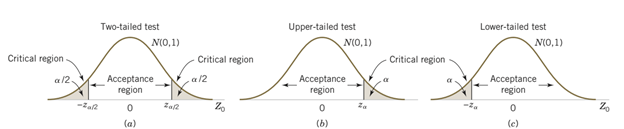
\includegraphics[width=6.5in,height=\textheight,keepaspectratio]{images/clipboard-3183526582.png}

}

\caption{\label{fig-7.5}Critical region for test of hypothesis (a)
Two-tailed test (b) Upper-tailed test (c) Lower-tailed test}

\end{figure}%

\textbf{Decision (P-value approach):} If calculated P-value for the test
statistic is less than or equal to \(\alpha\) then reject the \(H_0\)
otherwise do not reject.

\begin{itemize}
\item
  For lower tailed test, \(P\)-value \(=P(Z<z_0)\);
\item
  For upper tailed test, \(P\)-value \(=P(Z>z_0)\);
\item
  For two-tailed test, \(P\)-value \(P(Z>|z_0|)+P(Z<-|z_0|)]\).
\end{itemize}

\textbf{Problem 7.4} State the null and alternative hypothesis in each
case.

a) A hypothesis test will be used to potentially provide evidence that
the population mean is more than 10.

b) A hypothesis test will be used to potentially provide evidence that
the population mean is not equal to 7.

c) A hypothesis test will be used to potentially provide evidence that
the population mean is less than 5.\\

\textbf{Problem 7.5 (a)} For the hypothesis test H0: μ = 10 against H1:μ
\textgreater10 and variance known, calculate the P-value for each of the
following test statistics.

(i) \(z_0 = 2.05\) (ii) \(z_0 = - 1.84\) (iii) \(z_0 = 0.4\)\\

\ul{Solution 7.5 (a):} Since this is an upper-tailed test so

(i) P-value=\(P(Z>2.05)=P(Z<-2.05)=0.0202\)

(ii) P-value=\(P(Z>-1.84)=P(Z<1.84)=0.9671\)

(iii) P-value=\(P(Z>0.4)=P(Z<-0.4)=0.3446\)

\textbf{Problem 7.5 (b)} For the hypothesis test H0: μ = 5 against H1: μ
\textless5 and variance known, calculate the P-value for each of the
following test statistics. (i) \(z_0 = 2.05\) (ii) \(z_0 = - 1.84\)
(iii) \(z_0 = 0.4\)

\ul{Solution 7.5 (b):} Since this is an lower-tailed test so

(i) P-value=\(P(Z<2.05)=0.9798\).

(ii) P-value=\(P(Z<-1.84)=0.03288\).

(iii) do it yourself.

\textbf{Problem 7.5 (c)} For the hypothesis test H0:μ = 7 against H1: μ
≠ 7 and variance known, calculate the P-value for each of the following
test statistics.

\begin{enumerate}
\def\labelenumi{(\roman{enumi})}
\tightlist
\item
  \(z_0 = 2.05\) (ii) \(z_0 = - 1.84\) (iii) \(z_0 = 0.4\)
\end{enumerate}

\ul{Solution 7.5 (c):} Since this is an two-tailed test so

(i) P-value=\(P(Z>2.05)+P(Z<-2.05)=2P(Z<-2.05)=0.0404\).

(ii) P-value=\(P(Z<-1.84)+P(Z>1.84)=2P(Z<-1.84)=0.0658\).

(iii) do it yourself.

\textbf{Problem 7.6} The life in hours of a battery is known to be
approximately normally distributed with standard deviation \(\sigma=\)
1.25 hours. A random sample of 10 batteries has a mean life of
\(\bar x=\) 40.5 hours. \textbf{Conduct} a hypothesis test to justify
the claim that battery life exceeds 40 hours.

\textbf{Problem 7.7} A bearing used in an automotive application is
supposed to have a nominal inside diameter of 1.5 inches. A random
sample of 25 bearings is selected, and the average inside diameter of
these bearings is 1.4975 inches. Bearing diameter is known to be
normally distributed with standard deviation \(\sigma\) = 0.01 inch.
\textbf{Test} the hypothesis \(H_0:\mu = 1.5\) . versus
\(H_1:\mu \ne 1.5\) using \(\alpha = 0.01\).

\ul{Solution 7.7:}

Let \(X\) be the inside diameter of the bearings (in inches)

\textbf{Given},

Sample size, \(n=25\);

Sample mean \(\bar x =1.4975\) inches; Population SD, \(\sigma =0.01\)
inch.

\textbf{Hypotheses:}

\[H_0: \mu =1.5\]

\[H_1: \mu \ne 1.5 \ \ (two-tailed)\]

\textbf{Test statistic:} Since X follows normal distribution and
\(\sigma\) is known so the test statistic is:

\[z_0=\frac{\bar x-\mu_0}{\sigma/\sqrt n}=\frac{1.4975-1.5}{0.01/\sqrt 25}=-1.25\]

\textbf{Critical value:} At \(\alpha=0.05\),

\[-z_{\alpha/2}=- 1.96\ \ \ and \ \ \  z_{\alpha/2}=1.96\]

\textbf{Decision:} Since \(z_0\) does not fall in critical region so do
not reject the \(H_0\).

\textbf{Conclusion:} We can conclude the the mean inside diameter of the
bearing is 1.5 inches based on thie sample data.

\textbf{Problem 7.8} The manufacturer of the X-15 steel-belted radial
truck tire claims that the mean mileage the tire can be driven before
the tread wears out is 60,000 miles. Assume the mileage wear follows the
normal distribution and the standard deviation of the distribution is
5,000 miles. Crosset Truck Company bought 48 tires and found that the
mean mileage for its trucks is 59,500 miles. Is Crosset's experience
different from that claimed by the manufacturer at the 0.05 significance
level?

\subsubsection{One sample t-test}\label{one-sample-t-test}

When sampling is from a \textbf{normally distributed population} or
\textbf{sample size is sufficiently large} and t\textbf{he population
variance is unknown}, the test statistic for testing \(H_0: \mu=\mu_0\)
at \(\alpha\) is

\[t=\frac{\bar x-\mu_0}{s /\sqrt n}\]

Test statistic \(t\) follows a Student's 𝑡 distribution with \((n - 1)\)
degrees of freedom.

\textbf{Decision (Critical value approach):} If calculated \(t\) falls
in rejection region (CR) , then reject \(H_0\) . Otherwise, do not
reject \(H_0\).

\begin{itemize}
\item
  For lower tailed test, reject \(H_0\) if \(t<-t_\alpha\) ;
\item
  For upper tailed test, reject \(H_0\) if \(t> t_\alpha\) ;
\item
  For two-tailed test, reject \(H_0\) if \(t<-t_{\alpha/2}\) or
  \(t>t_{\alpha/2}\) .
\end{itemize}

\textbf{Problem 10.4} Annual per capita consumption of milk is 21.6
gallons (\emph{Statistical Abstract of the United States: 2006}). Being
from the Midwest, you believe milk consumption is higher there and wish
to support your opinion. A sample of 16 individuals from the Midwestern
town of Webster City showed a sample mean annual consumption of 24.1
gallons with a standard deviation of \(s=4.8\) .

a) Develop a hypothesis test that can be used to determine whether the
mean annual consumption in Webster City is higher than the national
mean.

b) Test the hypothesis at \(\alpha=0.05\) .

c) Draw a conclusion.

\textbf{Problem 10.5} The mean length of a small counterbalance bar is
43 millimeters. The production supervisor is concerned that the
adjustments of the machine producing the bars have changed. He asks the
Engineering Department to investigate. Engineer selects a random sample
of 10 bars and measures each. The results are reported below in
millimeters.

42, 39, 42, 45, 43, 40, 39, 41, 40, 42

Is it reasonable to conclude that there has been a change in the mean
length of the bars?

\subsection{Normality test}\label{normality-test}

In parametric (distribution based ) hypothesis test the checking
normality assumption of study variable is a common practice especially
when the sample size is small (\(n<30\)). For large samples, the
\textbf{Central Limit Theorem (CLT)} often makes this test robust to
non-normality.

The normality assumption is checked in two ways:

a) Graphically

b) Numerically using some normality tests

\textbf{a) Graphical procedure to check normality}

We often plot the data (i.e., histogram, density plot, boxplot) to
explore so called bell-shaped of the data. But the most popular and
effective way to check normality is \textbf{Q-Q plot (Quantile- Quantile
plot).}

\textbf{b) Normality test}

A number of normality tests are available; of them a common test is
\textbf{Shapiro-Wilk} test of normality suitable for small to medium
sample size (3 to 5000) (Shapiro and Wilk 1965; Royston 1982).

\textbf{Shapiro-Wilk Test Statistic W}

\[W=\frac{(\sum_{i=1}^n a_i x_{(i)})^2}{\sum_{i=1}^n (x_i-\bar x)^2}\]

Where,

\begin{itemize}
\item
  \(x_{(i)}\) : the \(i^{th}\) \textbf{order statistic} (i.e., the
  \emph{i}-th smallest value in the sample)
\item
  \(\bar x\): the \textbf{sample mean}
\item
  \(a_i\) : constants calculated based on the \textbf{expected values
  and variances} of order statistics from a \textbf{standard normal
  distribution (}Tabulated in Shapiro Wilk Table)
\item
  \(n\): sample size
\end{itemize}

\textbf{Hypotheses:}

\begin{itemize}
\item
  \textbf{Null Hypothesis} \(H_0\): The data are \textbf{normally
  distributed}.
\item
  \textbf{Alternative} \(H_1\): The data are \textbf{not normally
  distributed}.
\end{itemize}

We reject \(H_0\) if the \textbf{p-value} is less than our significance
level (e.g., 0.05).

Almost all statistical software and package routinely provide the
\textbf{Shapiro-Wilk} test.

In \textbf{R} Shapiro-Wilk test is available as \texttt{shapiro.test} .

\begin{verbatim}

    Shapiro-Wilk normality test

data:  uniform.data
W = 0.93903, p-value = 0.0001683
\end{verbatim}

The p-value\textless0.05 implies (reject \(H_0\)) that the data is not
normally distributed.

\begin{verbatim}

    Shapiro-Wilk normality test

data:  normal.data
W = 0.99212, p-value = 0.83
\end{verbatim}

The p-value\textgreater0.05 implies (do not reject \(H_0\)) that the
data is normally distributed.

\bookmarksetup{startatroot}

\chapter{Simple Linear Regression and
Correlation}\label{simple-linear-regression-and-correlation}

\section{Simple linear regression
(SLR)}\label{simple-linear-regression-slr}

In regression analysis we try to estimate or predict the
\textbf{outcome/ response} of one variable (dependent variable) on the
basis of other variables (independent variable). For example, sales of
certain product depends of price, advertising cost, quality of the
product, brand etc.

It involves developing a mathematical model or equation that describes
the relationship between the \textbf{dependent variable} and the
\textbf{independent variables.}

In the following section we will discuss about the \textbf{Simple linear
regression (SLR)} where a independent variable and a dependent variable
are involved.

\subsection{\texorpdfstring{\textbf{Population regression function
(PRF)}}{Population regression function (PRF)}}\label{population-regression-function-prf}

\begin{equation}\phantomsection\label{eq-PRF}{y_i=\beta_0+\beta_1 x_i+\epsilon_i \hspace{10pt} ; i=1,2,3,..., N}\end{equation}

Where,

\(y\)= dependent variable

\(x\)= independent variable

\(\beta_0\) =y-intercept

\(\beta_1\)= slope of the line/ regression coefficient

\(\varepsilon\) = error variable

\textbf{Assumptions}

\begin{enumerate}
\def\labelenumi{\roman{enumi})}
\item
  The errors are \emph{independently}, \emph{identically} normally
  distributed with \textbf{constant variance} \(\sigma_\varepsilon ^2\)
  that is
  \(\varepsilon_i \overset{\text{i.i.d.}}{\sim} \mathcal{N}(0, \sigma_\epsilon^2)\)
  .
\item
  The independent variable should not be correlated with the error term
  (no endogeneity)
\end{enumerate}

Taking conditional expectation of of \textbf{PRF} for a given \(x_i\) we
have

\begin{equation}\phantomsection\label{eq-expectedprf}{E(y_i/x_i)=\beta_0+\beta_1 x_i }\end{equation}

From sample data we have to estimate \(E(y_i/x_i)\) which is equivalent
to estimate \(\beta_0\) and \(\beta_1\).

\subsection{\texorpdfstring{Ordinary least square (OLS) estimate of
\(E(y_i/x_i)\)}{Ordinary least square (OLS) estimate of E(y\_i/x\_i)}}\label{ordinary-least-square-ols-estimate-of-ey_ix_i}

Let we have \(n\) pairs of sample data:
\(\{X,Y\}=\{ (x_1,y_1), (x_2,y_2),..., (x_n, y_n) \}\). From the sample
data suppose the \textbf{estimated regression line of} \(E(y_i/x_i)\)
\textbf{is}

\[\hat y_i= \hat \beta_0+\hat \beta_1 x_i \hspace {10pt}; i=1,2,....,n\]

So,

\[y_i=\hat y_i +e_i \hspace{10pt} ; i=1,2, ..., n\]

Where, \(e_i\) is the \textbf{estimated error} or \textbf{residual.}

Now, the \textbf{residuals sum of square (RSS)} is given as:

\begin{equation}\phantomsection\label{eq-ssr}{RSS=\sum_{i=1}^n e_i^2=\sum_{i=1}^n (y_i-\hat y_i)^2=\sum_{i=1}^n (y_i-\hat \beta_0-\hat \beta_1x_i)^2}\end{equation}

In \textbf{OLS} method we \emph{minimize} the \textbf{RSS}with respect
to \(\hat \beta_0\) and \(\hat \beta_1\). To minimize \textbf{RSS}we
have to set two equations using \emph{partial derivative:}

\begin{equation}\phantomsection\label{eq-ols1}{\frac{\delta \hspace{1pt} (RSS)}{\delta \hat \beta_0}=0}\end{equation}

\begin{equation}\phantomsection\label{eq-ols2}{\frac{\delta \hspace{1pt} (RSS)}{\delta \hat \beta_1}=0}\end{equation}

By solving the two equations we will have the \textbf{OLS estimates} of
\(\beta_0\) and \(\beta_1\) as follows:

\[\hat \beta_0=\bar y-\hat \beta_1 \bar x\] and

\[\hat \beta_1=\frac{\sum_{i=1}^n (x_i-\bar x)(y_i-\bar y)} {\sum_{i=1}^n (x_i-\bar x)^2}=\frac{s_{xy}}{s^2_x}\]

Or,

\[\hat \beta_1=r_{xy} \left (\frac{s_y}{s_x}\right )\]

Thus, the \textbf{estimated regression} line is given by

\[\hat y_i=\hat \beta_0+\hat \beta_1 x_i\]

\subsection{\texorpdfstring{Point prediction of \(y\) for a give
\(x\)}{Point prediction of y for a give x}}\label{point-prediction-of-y-for-a-give-x}

Given \(x=x_g\). Then the estimated \(y\) for given \(x\) is

\[\hat y_g=\hat \beta _0+\hat \beta_1 \times x_g\]

\subsection{Partition of sum squares}\label{partition-of-sum-squares}

\begin{enumerate}
\def\labelenumi{\roman{enumi})}
\tightlist
\item
  Total sum of square,
\end{enumerate}

\[SS(Total)=\sum_{i=1}^n (y_i-\bar y)^2=(n-1) s^2_y\]

\begin{enumerate}
\def\labelenumi{\roman{enumi})}
\setcounter{enumi}{1}
\tightlist
\item
  Regression sum of square,
\end{enumerate}

\[SSR=\sum_{i=1}^n (\hat y_i-\bar y)^2 \]

In the case of \textbf{SLR}, SSR can be written as
\[SSR=\hat \beta_1^2\sum_{i=1}^n (x_i-\bar x)^2=\hat \beta_1^2 (n-1)s_x^2\]

\begin{enumerate}
\def\labelenumi{\roman{enumi})}
\setcounter{enumi}{2}
\tightlist
\item
  Sum of square of error,
\end{enumerate}

\[SSE=\sum_{i=1}^n (y_i-\hat y_i)^2=SS(Total)-SSR\]

\subsection{Coefficient of determination (Goodness of
fit)}\label{coefficient-of-determination-goodness-of-fit}

\[R^2=\frac{SSR}{SS(Total)}  \hspace{10pt}; \hspace{10pt} 0\le R^2\le1 \]

\textbf{Interpretation:} The \(R^2\) explains the amount of variation in
\(Y\) (dependent variable) by the estimated model.

In the case of \textbf{SLR,}

\[R^2=r_{xy}^2=\frac{s^2_{xy}}{s_x^2 \times s^2_y}\]

We can also write \(R^2\) as:

\[R^2=\frac{\hat \beta_1^2 \sum(x-\bar x)^2}{\sum(y-\bar y)^2}\]

\subsection{Some problems on SLR}\label{some-problems-on-slr}

\textbf{Problem 15.3 :} The owner of a paint store was attempting to
analyse the relationship between advertising and sales, and recorded the
monthly advertising budget (\$'000) and the sales (\$m) for a sample of
12 months. The data are listed here:

\begin{longtable}[]{@{}
  >{\raggedright\arraybackslash}p{(\linewidth - 24\tabcolsep) * \real{0.2099}}
  >{\centering\arraybackslash}p{(\linewidth - 24\tabcolsep) * \real{0.0617}}
  >{\centering\arraybackslash}p{(\linewidth - 24\tabcolsep) * \real{0.0617}}
  >{\centering\arraybackslash}p{(\linewidth - 24\tabcolsep) * \real{0.0617}}
  >{\centering\arraybackslash}p{(\linewidth - 24\tabcolsep) * \real{0.0617}}
  >{\centering\arraybackslash}p{(\linewidth - 24\tabcolsep) * \real{0.0617}}
  >{\centering\arraybackslash}p{(\linewidth - 24\tabcolsep) * \real{0.0741}}
  >{\centering\arraybackslash}p{(\linewidth - 24\tabcolsep) * \real{0.0617}}
  >{\centering\arraybackslash}p{(\linewidth - 24\tabcolsep) * \real{0.0741}}
  >{\centering\arraybackslash}p{(\linewidth - 24\tabcolsep) * \real{0.0617}}
  >{\centering\arraybackslash}p{(\linewidth - 24\tabcolsep) * \real{0.0617}}
  >{\centering\arraybackslash}p{(\linewidth - 24\tabcolsep) * \real{0.0741}}
  >{\centering\arraybackslash}p{(\linewidth - 24\tabcolsep) * \real{0.0741}}@{}}
\toprule\noalign{}
\endhead
\bottomrule\noalign{}
\endlastfoot
\textbf{Advertising} & 23 & 46 & 60 & 54 & 28 & 33 & 25 & 31 & 36 & 88 &
95 & 99 \\
\textbf{Sales} & 8 & 11 & 13 & 13 & 8.9 & 10.7 & 9 & 10.4 & 11 & 14 &
14.4 & 15.9 \\
\end{longtable}

i) \textbf{Identify} the dependent and independent variable.

ii) \textbf{Plot} the data. Is it appear to be linear?

iii) Now, \textbf{fit}/ \textbf{estimate} a linear regression line.

iv) \textbf{Interpret} the regression/slope coefficient.

v) \textbf{Predict} the sales for the advertising cost \$70, 000.

vi) \textbf{Comment} about goodness of fit of the estimated model.

\textbf{Problem 15.4} \textbf{Age and Blood Pressure.}The ages (in
years) of 10 men and their systolic blood pressures (in millimeters of
mercury).

\begin{longtable}[]{@{}
  >{\raggedright\arraybackslash}p{(\linewidth - 20\tabcolsep) * \real{0.4118}}
  >{\centering\arraybackslash}p{(\linewidth - 20\tabcolsep) * \real{0.0588}}
  >{\centering\arraybackslash}p{(\linewidth - 20\tabcolsep) * \real{0.0588}}
  >{\centering\arraybackslash}p{(\linewidth - 20\tabcolsep) * \real{0.0588}}
  >{\centering\arraybackslash}p{(\linewidth - 20\tabcolsep) * \real{0.0588}}
  >{\centering\arraybackslash}p{(\linewidth - 20\tabcolsep) * \real{0.0588}}
  >{\centering\arraybackslash}p{(\linewidth - 20\tabcolsep) * \real{0.0588}}
  >{\centering\arraybackslash}p{(\linewidth - 20\tabcolsep) * \real{0.0588}}
  >{\centering\arraybackslash}p{(\linewidth - 20\tabcolsep) * \real{0.0588}}
  >{\centering\arraybackslash}p{(\linewidth - 20\tabcolsep) * \real{0.0588}}
  >{\raggedright\arraybackslash}p{(\linewidth - 20\tabcolsep) * \real{0.0588}}@{}}
\toprule\noalign{}
\endhead
\bottomrule\noalign{}
\endlastfoot
\textbf{Age} & 16 & 25 & 39 & 45 & 49 & 64 & 70 & 29 & 57 & 22 \\
\textbf{Systolic blood pressure (SBP)} & 109 & 128 & 143 & 145 & 180 &
185 & 185 & 199 & 175 & 118 \\
\end{longtable}

\begin{enumerate}
\def\labelenumi{\roman{enumi})}
\item
  \textbf{Identify} the dependent and independent variable.
\item
  \textbf{Plot} the data. Is it appear to be linear?
\item
  Now, \textbf{fit}/ \textbf{estimate} a linear regression line.
\item
  \textbf{Interpret} the regression/slope coefficient.
\item
  \textbf{Predict} the SBP for the age of a person is 40 years .
\item
  \textbf{Comment} about goodness of fit of the estimated model.
\end{enumerate}

\ul{\textbf{Solution:}}

Let, \(Y\)=Systolic blood pressure, SBP and \(X\) = age (in years)

\textbf{i)} Here SBP is dependent variable and age is independent
variable

\textbf{ii) Scatter plot of Age versus SBP}

\begin{figure}

\pandocbounded{
\includegraphics[keepaspectratio]{7Linear_regression_files/figure-pdf/fig-slr-1.pdf}}

\caption{\label{fig-slr}Sacter plot of Age and SBP}

\end{figure}%

The scatter plot appears to be linear.

\textbf{iii)} Let the estimated regression line is :

\[\hat y_i=\hat \beta_0 +\hat \beta_1 x_i \hspace{40pt} (1)\]

From sample data;

\(n=10, \sum x =416  , \sum y=1512 , \sum x^2 =20398\),

\(\sum y^2=237414, \sum xy=67977\)

\(\bar x=41.6 , \hspace{10pt} \bar y=151.2\)

So,

\[s_{xy}=\frac{\sum xy-n \cdot \bar x \cdot \bar y}{n-1}=\frac{67977-10\times 41.6\times 151.2}{10-1}=564.2\]

\[s^2_x=\frac{\sum x^2 -n\times \bar x^2}{n-1}=343.6\]

\[s^2_y=\frac{\sum y^2 -n\times \bar y^2}{n-1}=977.7333\]

Hence,

\[\hat \beta_1=\frac{s_{xy}}{s^2_x}=\frac{564.2}{343.6}=1.642026\approx 1.642\]

and,

\[\hat \beta_0=\bar y-\hat \beta_1 \bar x=151.2-1.642026\times41.6=82.89172\approx82.8917 \]

\[\therefore \hat y_i=82.8917+1.642\hspace{3pt}x_i \hspace{5pt}\]

\begin{enumerate}
\def\labelenumi{\roman{enumi})}
\setcounter{enumi}{3}
\tightlist
\item
  \textbf{Interpretation of the regression/slope coefficient:}
\end{enumerate}

Here \(\hat \beta_1=1.642\) implies that as one year increases, the SBP
will increases by 1.642 Hg m on average.

\begin{enumerate}
\def\labelenumi{\alph{enumi})}
\setcounter{enumi}{21}
\tightlist
\item
  \textbf{Predict the SBP for the age of a person is 40 years:}
\end{enumerate}

For \(x=40\) years, the predicted SBP (in Hg m) is

\(\hat y_g =82.8917+1.642\times 40=148.5728\) Hg m

\begin{enumerate}
\def\labelenumi{\roman{enumi})}
\setcounter{enumi}{5}
\tightlist
\item
  \textbf{Comment about goodness of fit of the estimated model:}
\end{enumerate}

The goodness of fit measure is

\[R^2=\frac{s^2_{xy} }{s^2_x \cdot s^2_y}=\frac{(564.2)^2}{(343.6)(977.7333)}=0.9475\]

Hence, \(R^2=0.9475\) implies that 94.75\% variation in ``SBP'' can be
explained by the estimated model.

\section{Correlation}\label{correlation}

In SLR we assume \(Y\) as a random variable but the independent
regressor variable \(x\) is a physical or scientific variable but not a
random variable. In many situations both \(X\) and \(Y\) are treated as
stochastic or random variable with a joint density function \(f(x,y)\)
(if both \(X\) and \(Y\) are continuous random variables).

\textbf{Correlation} analysis study the \emph{degree} and
\emph{direction} of \emph{linear relationship} between two quantitative
random variables.

The numerical value of correlation is called \textbf{correlation
coefficient} or \textbf{Pearson correlation coefficient}.

\subsection{Population correlation
coefficient}\label{population-correlation-coefficient}

The population correlation coefficient is denoted by \(\rho\) and
defined as:

\[\rho=\frac{\sigma_{XY}}{\sigma_X \sigma_Y} \ \ \ \ ; \ \ -1\le \rho \le +1\]
where,
\(\sigma_{X,Y}=Cov (X,Y)=E[(X-\mu_X)(Y-\mu_Y)]=E(XY)-\mu_X \mu_Y\)

\subsection{Sample correlation
coefficient}\label{sample-correlation-coefficient}

The \(\rho\) is estimated from sample data by \textbf{sample correlation
coefficient} \(r\), where

\[r=\frac{s_{XY}}{s_Y s_Y}\]

To understand the nature and to measure the \textbf{linear relationship
(correlation)} between two quantitative variable we use some techniques.
In the following section we will discuss about that.

\subsection{Scatter plot: Graphical method to explore
correlation}\label{scatter-plot-graphical-method-to-explore-correlation}

A \textbf{scatter plot} shows the relationship between two quantitative
variables measured for the same individuals. The values of one variable
appear on the horizontal axis, and the values of the other variable
appear on the vertical axis. Each individual in the data appears as a
point on the graph.

\begin{itemize}
\tightlist
\item
  A scatterplot \emph{displays} the strength, direction, and form of the
  relationship between two quantitative variables (\emph{see}
  Figure~\ref{fig-scatter}).
\end{itemize}

\begin{figure}

\centering{

\pandocbounded{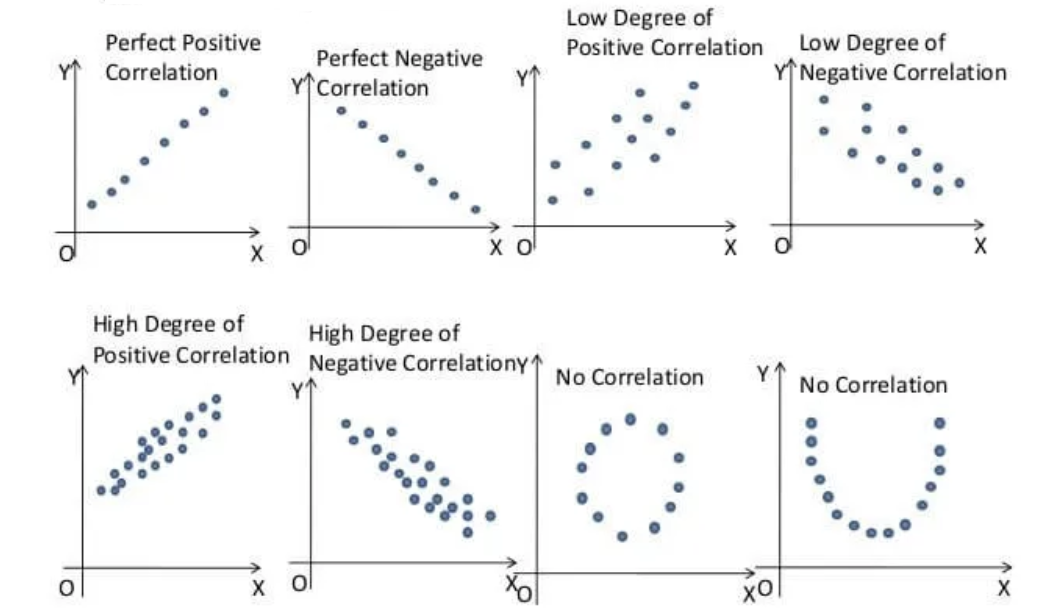
\includegraphics[keepaspectratio]{Scatter.png}}

}

\caption{\label{fig-scatter}Types of correlations that can be
represented using a scatter plot}

\end{figure}%

Lets draw a scatter plot for the following data.

\begin{longtable}[]{@{}lrrrrrrrrrr@{}}

\caption{\label{tbl-xydata}Data}

\tabularnewline

\toprule\noalign{}
& 1 & 2 & 3 & 4 & 5 & 6 & 7 & 8 & 9 & 10 \\
\midrule\noalign{}
\endhead
\bottomrule\noalign{}
\endlastfoot
x & 2 & 5 & 1 & 3 & 4 & 1 & 5 & 3 & 4 & 2 \\
y & 50 & 57 & 41 & 54 & 54 & 38 & 63 & 48 & 59 & 46 \\

\end{longtable}

\begin{figure}

\centering{

\pandocbounded{
\includegraphics[keepaspectratio]{7Linear_regression_files/figure-pdf/fig-scatterplot-1.pdf}}

}

\caption{\label{fig-scatterplot}Sctter plot between X and Y}

\end{figure}%

In fact, the scatter lot suggests that a straight line could be used as
an approximation of the relationship. However \emph{coefficient of
correlation} as descriptive measures which provide \emph{direction} and
\emph{strength} of the linear relationship between two variables.

\subsection{Properties of coefficient of
correlation}\label{properties-of-coefficient-of-correlation}

\begin{enumerate}
\def\labelenumi{\arabic{enumi}.}
\item
  The value of \(\rho\) is always between -1 and 1 inclusive. That is
  \(-1\le \rho\le+1\).
\item
  If all values of either variable are converted to a different scale,
  the value of \(\rho\) does not change (NOT affected by change of
  \emph{origin} and \emph{scale}).
\item
  The value of \(\rho\) is not affected by the choice of X or Y.
  Interchange all x values and y values, and the value of \(\rho\) will
  not change (\(\rho\) is a symmetric measure).
\item
  \(\rho\) measures the strength of a \emph{linear relationship}. It is
  not designed to measure the strength of a relationship that is not
  linear.
\item
  \(\rho\) is very sensitive to outliers in the sense that a single
  outlier could dramatically affect its value.
\end{enumerate}

\begin{tcolorbox}[enhanced jigsaw, bottomrule=.15mm, toprule=.15mm, title=\textcolor{quarto-callout-note-color}{\faInfo}\hspace{0.5em}{Proof of \(-1\le\rho\le+1\)}, bottomtitle=1mm, colframe=quarto-callout-note-color-frame, coltitle=black, rightrule=.15mm, toptitle=1mm, colbacktitle=quarto-callout-note-color!10!white, titlerule=0mm, breakable, arc=.35mm, leftrule=.75mm, opacitybacktitle=0.6, opacityback=0, colback=white, left=2mm]

From Cauchy--Schwarz Inequality we know that,

\[(E[XY])^2\le E[X^2] E[Y^2]\]

Now center the variables \(X\) and \(Y\) with respect to their mean we
have,

\[(E[(X-\mu_X)(Y-\mu_Y)])^2 \le E[(X-\mu_X)^2] E[(Y-\mu_Y)^2]\]

\[\Rightarrow [Cov(X,Y)]^2 \le Var(X)  \cdot Var(Y)\]

\[\Rightarrow (\sigma_{XY})^2 \le \sigma^2_X \sigma^2_Y \]

\[\Rightarrow | \sigma_{XY}| \le \sigma_X \sigma_Y\]

\[\Rightarrow |\frac{\sigma_{XY}}{\sigma_X \sigma_Y}\le 1|\]

\[\Rightarrow |\rho|\le 1\]

Which implies that \(-1 \le \rho\le +1\).

\end{tcolorbox}

\begin{tcolorbox}[enhanced jigsaw, bottomrule=.15mm, toprule=.15mm, title=\textcolor{quarto-callout-note-color}{\faInfo}\hspace{0.5em}{Effect of change of origin and scale on \(\rho\)}, bottomtitle=1mm, colframe=quarto-callout-note-color-frame, coltitle=black, rightrule=.15mm, toptitle=1mm, colbacktitle=quarto-callout-note-color!10!white, titlerule=0mm, breakable, arc=.35mm, leftrule=.75mm, opacitybacktitle=0.6, opacityback=0, colback=white, left=2mm]

Let, \(U=\frac{X-a}{b}\) and \(V=\frac{Y-c}{d}\). Here \(a,b,c,d\) are
any arbitrary real numbers.

We have to prove that, \(\rho_{XY}=\rho_{UV}\).

\textbf{Proof:}

So we have,

\(X=a+bU\) ; and \(\bar X =a+b \bar U\). Similarly

\(Y=c+dV\) ; and \(\bar Y=c+d \bar V\)

Now,

\(\sigma_{XY}=\frac {\sum(X-\bar X)(Y-\bar Y)}{N}=\frac{bd\sum(U-\bar U)(V-\bar V)}{N}=bd\times \sigma_{UV}\)

\(\sigma_X^2=Var(X)=Var(a+bU)=b^2 Var(U)=b^2 \sigma^2_U\)

Hence, \(\sigma_X=b\sigma_U\) (standard deviation is always \(\ge0\)).

Similarly, \(\sigma_Y=d\sigma_V\)

Finally we have,

\[\rho_{XY}=\frac{\sigma_{XY}}{\sigma_X \sigma_Y}=\frac{bd\times \sigma_{UV}}{b\sigma_U \times d\sigma_V}=\frac{\sigma_{UV}}{\sigma_U \sigma_V}=\rho_{UV} \ \ \ \  (PROVED.)\]

\end{tcolorbox}

\subsection{Interpretation of correlation
coefficient}\label{interpretation-of-correlation-coefficient}

\begin{enumerate}
\def\labelenumi{(\alph{enumi})}
\item
  \(r=-1\) implies \emph{perfect negative} correlation,
\item
  \(r=+1\) implies \emph{perfect positive} correlation,
\item
  \(r\approx 0\) implies no correlation or very weak correlation,
\item
  As \(r\) close to \(-1\) , the degree of \emph{negative} correlation
  becomes stronger,
\item
  As \(r\) close to \(+1\) , the degree of \emph{positive} correlation
  becomes stronger.
\end{enumerate}

\subsection{Computing the Coefficient of
Correlation}\label{computing-the-coefficient-of-correlation}

Let us compute sample correlation coefficient between \(X\) and \(Y\)
from Table~\ref{tbl-xydata}.

Here, \(n=10 ; \sum x=30 ; \sum y =510\).

\(\sum xy =x_1y_1+x_2y_2+ \cdot \cdot \cdot+x_ny_n= 1629\)

\(\sum x^2=2^2+5^2 +...+2^2=110\)

\(\sum y^2=50^2+57^2 +...+46^2=26576\)

\(\bar x =3\)

\(\bar y =51\)

So,

\[s_X=\sqrt { \frac{\sum x^2 -n \ \  \bar x^2}{n-1}}=1.490712\]

\[s_Y=\sqrt { \frac{\sum y^2 -n \ \ \bar y^2}{n-1}}=7.930252\]

\[s_{XY}=\frac{\sum xy -n \ \ \bar x \ \ \bar y }{n-1}=11\]

Hence,

\[r=\frac{s_{XY}}{s_X \times s_Y}=\frac{11}{1.490712\times 7.930252}=0.9305\]

which is close to 1. So the correlation between \(X\) and \(Y\) is
\emph{strong} and \emph{positive}.

\subsection{Exercises: Constructing a Scatter Plot and Determining
Correlation}\label{exercises-constructing-a-scatter-plot-and-determining-correlation}

In Exercises 1--4, (a) display the data in a scatter plot, (b) calculate
the sample correlation coefficient \(r\), and (c) describe the type of
correlation and interpret the correlation in the context of the data.

\begin{enumerate}
\def\labelenumi{\arabic{enumi}.}
\tightlist
\item
  \textbf{Age and Blood Pressure.} The ages (in years) of 10 men and
  their systolic blood pressures (in millimeters of mercury) (Larson and
  Farber 2015, 482)
\end{enumerate}

\begin{longtable}[]{@{}
  >{\raggedright\arraybackslash}p{(\linewidth - 20\tabcolsep) * \real{0.3902}}
  >{\centering\arraybackslash}p{(\linewidth - 20\tabcolsep) * \real{0.0610}}
  >{\centering\arraybackslash}p{(\linewidth - 20\tabcolsep) * \real{0.0610}}
  >{\centering\arraybackslash}p{(\linewidth - 20\tabcolsep) * \real{0.0610}}
  >{\centering\arraybackslash}p{(\linewidth - 20\tabcolsep) * \real{0.0610}}
  >{\centering\arraybackslash}p{(\linewidth - 20\tabcolsep) * \real{0.0610}}
  >{\centering\arraybackslash}p{(\linewidth - 20\tabcolsep) * \real{0.0610}}
  >{\centering\arraybackslash}p{(\linewidth - 20\tabcolsep) * \real{0.0610}}
  >{\centering\arraybackslash}p{(\linewidth - 20\tabcolsep) * \real{0.0610}}
  >{\centering\arraybackslash}p{(\linewidth - 20\tabcolsep) * \real{0.0610}}
  >{\raggedright\arraybackslash}p{(\linewidth - 20\tabcolsep) * \real{0.0610}}@{}}
\toprule\noalign{}
\endhead
\bottomrule\noalign{}
\endlastfoot
\textbf{Age, x} & 16 & 25 & 39 & 45 & 49 & 64 & 70 & 29 & 57 & 22 \\
\textbf{Systolic blood pressure, y} & 109 & 122 & 143 & 132 & 199 & 185
& 199 & 130 & 175 & 118 \\
\end{longtable}

\begin{enumerate}
\def\labelenumi{\arabic{enumi}.}
\setcounter{enumi}{1}
\tightlist
\item
  \textbf{Driving Speed and Fuel Efficiency.} A department of
  transportation's study on driving speed and miles per gallon for
  midsize automobiles resulted in the following data (Anderson 2020a,
  149):
\end{enumerate}

\begin{longtable}[]{@{}
  >{\raggedright\arraybackslash}p{(\linewidth - 20\tabcolsep) * \real{0.3590}}
  >{\centering\arraybackslash}p{(\linewidth - 20\tabcolsep) * \real{0.0641}}
  >{\centering\arraybackslash}p{(\linewidth - 20\tabcolsep) * \real{0.0641}}
  >{\centering\arraybackslash}p{(\linewidth - 20\tabcolsep) * \real{0.0641}}
  >{\centering\arraybackslash}p{(\linewidth - 20\tabcolsep) * \real{0.0641}}
  >{\centering\arraybackslash}p{(\linewidth - 20\tabcolsep) * \real{0.0641}}
  >{\centering\arraybackslash}p{(\linewidth - 20\tabcolsep) * \real{0.0641}}
  >{\centering\arraybackslash}p{(\linewidth - 20\tabcolsep) * \real{0.0641}}
  >{\centering\arraybackslash}p{(\linewidth - 20\tabcolsep) * \real{0.0641}}
  >{\centering\arraybackslash}p{(\linewidth - 20\tabcolsep) * \real{0.0641}}
  >{\centering\arraybackslash}p{(\linewidth - 20\tabcolsep) * \real{0.0641}}@{}}
\toprule\noalign{}
\endhead
\bottomrule\noalign{}
\endlastfoot
\textbf{Speed (Miles per Hour)} & 30 & 50 & 40 & 55 & 30 & 25 & 60 & 25
& 50 & 55 \\
\textbf{Miles per Gallon} & 28 & 25 & 25 & 23 & 30 & 32 & 21 & 35 & 26 &
25 \\
\end{longtable}

\begin{enumerate}
\def\labelenumi{\arabic{enumi}.}
\setcounter{enumi}{2}
\tightlist
\item
  Are the marks one receives in a course related to the amount of time
  spent studying the subject? To analyze this mysterious possibility, a
  student took a random sample of 10 students who had enrolled in an
  accounting class last semester. He asked each to report his or her
  mark in the course and the total number of hours spent studying
  accounting. These data are listed here (Keller 2014).
\end{enumerate}

\begin{longtable}[]{@{}
  >{\raggedright\arraybackslash}p{(\linewidth - 20\tabcolsep) * \real{0.2424}}
  >{\centering\arraybackslash}p{(\linewidth - 20\tabcolsep) * \real{0.0758}}
  >{\centering\arraybackslash}p{(\linewidth - 20\tabcolsep) * \real{0.0758}}
  >{\centering\arraybackslash}p{(\linewidth - 20\tabcolsep) * \real{0.0758}}
  >{\centering\arraybackslash}p{(\linewidth - 20\tabcolsep) * \real{0.0758}}
  >{\centering\arraybackslash}p{(\linewidth - 20\tabcolsep) * \real{0.0758}}
  >{\centering\arraybackslash}p{(\linewidth - 20\tabcolsep) * \real{0.0758}}
  >{\centering\arraybackslash}p{(\linewidth - 20\tabcolsep) * \real{0.0758}}
  >{\centering\arraybackslash}p{(\linewidth - 20\tabcolsep) * \real{0.0758}}
  >{\centering\arraybackslash}p{(\linewidth - 20\tabcolsep) * \real{0.0758}}
  >{\centering\arraybackslash}p{(\linewidth - 20\tabcolsep) * \real{0.0758}}@{}}
\toprule\noalign{}
\endhead
\bottomrule\noalign{}
\endlastfoot
\textbf{Study time} & 40 & 42 & 37 & 47 & 25 & 44 & 41 & 48 & 35 & 28 \\
\textbf{Marks} & 77 & 63 & 79 & 86 & 51 & 78 & 83 & 90 & 65 & 47 \\
\end{longtable}

\begin{enumerate}
\def\labelenumi{\arabic{enumi}.}
\setcounter{enumi}{3}
\tightlist
\item
  The owner of a paint store was attempting to analyse the relationship
  between advertising and sales, and recorded the monthly advertising
  budget (\$'000) and the sales (\$m) for a sample of 12 months. The
  data are listed here
\end{enumerate}

\begin{longtable}[]{@{}
  >{\raggedright\arraybackslash}p{(\linewidth - 24\tabcolsep) * \real{0.2099}}
  >{\centering\arraybackslash}p{(\linewidth - 24\tabcolsep) * \real{0.0617}}
  >{\centering\arraybackslash}p{(\linewidth - 24\tabcolsep) * \real{0.0617}}
  >{\centering\arraybackslash}p{(\linewidth - 24\tabcolsep) * \real{0.0617}}
  >{\centering\arraybackslash}p{(\linewidth - 24\tabcolsep) * \real{0.0617}}
  >{\centering\arraybackslash}p{(\linewidth - 24\tabcolsep) * \real{0.0617}}
  >{\centering\arraybackslash}p{(\linewidth - 24\tabcolsep) * \real{0.0741}}
  >{\centering\arraybackslash}p{(\linewidth - 24\tabcolsep) * \real{0.0617}}
  >{\centering\arraybackslash}p{(\linewidth - 24\tabcolsep) * \real{0.0741}}
  >{\centering\arraybackslash}p{(\linewidth - 24\tabcolsep) * \real{0.0617}}
  >{\centering\arraybackslash}p{(\linewidth - 24\tabcolsep) * \real{0.0617}}
  >{\centering\arraybackslash}p{(\linewidth - 24\tabcolsep) * \real{0.0741}}
  >{\centering\arraybackslash}p{(\linewidth - 24\tabcolsep) * \real{0.0741}}@{}}
\toprule\noalign{}
\endhead
\bottomrule\noalign{}
\endlastfoot
\textbf{Advertising} & 23 & 46 & 60 & 54 & 28 & 33 & 25 & 31 & 36 & 88 &
95 & 99 \\
\textbf{Sales} & 8 & 11 & 13 & 13 & 8.9 & 10.7 & 9 & 10.4 & 11 & 14 &
14.4 & 15.9 \\
\end{longtable}

\subsection{Coefficient of
determination}\label{coefficient-of-determination}

The coefficient of determination measures the amount of variation in the
dependent variable that is explained by the variation in the independent
variable.

For example, if \(r=0.8764\) between \(X\) and \(Y\) then
\textbf{coefficient of determination} \(r^2=(0.8764)^2 \approx 0.7681\).

\textbf{Interpretation:} The \(r^2=0.7681\) tells us that 76.81\%
variation in \(Y\) (dependent variable) can be explained by \(X\)
(independent variable).\\

\subsection{Correlation vs.~causation}\label{correlation-vs.-causation}

\emph{Correlation} does not always imply \emph{causation}. For example,

\begin{itemize}
\item
  A study(Messerli 2012) found that there was a significant
  (\(r=0.791\)) positive correlation between \emph{chocolate consumption
  per capita} and \emph{number of Nobel laureates per 10 million
  persons}. This does not necessarily implies that more a country
  consumes chocolate, more the chance of getting a Nobel prize. Rather
  differences in socioeconomic status from country to country and
  geographic and climatic factors may play some role to win a Nobel
  prize.
\item
  We might find that there is a positive correlation between the time
  spent driving on road and the number of accidents but this does not
  mean that spending more time on road causes accident.Because in that
  case, in order to avoid accidents one may drive fast so that time
  spent on road is less (Selvamuthu and Das 2024).
\end{itemize}

\subsection{Effect of outlier on correlation
coefficient}\label{effect-of-outlier-on-correlation-coefficient}

The correlation coefficient is heavily affected by outlier (see
Figure~\ref{fig-outlieronr1}). It changes the magnitude of the
correlation coefficient.

\begin{figure}

\centering{

\pandocbounded{
\includegraphics[keepaspectratio]{7Linear_regression_files/figure-pdf/fig-outlieronr1-1.pdf}}

}

\caption{\label{fig-outlieronr1}Effect of outlier on the magnitude of
correlation coefficient (r)}

\end{figure}%

Even sometime the outlier(s) can change the sign of the correlation
coefficient (see Figure~\ref{fig-outlieronr2}).

\begin{figure}

\centering{

\pandocbounded{
\includegraphics[keepaspectratio]{7Linear_regression_files/figure-pdf/fig-outlieronr2-1.pdf}}

}

\caption{\label{fig-outlieronr2}Effect of outlier on the sign of
correlation coefficient (r)}

\end{figure}%

\section{Rank correlation}\label{rank-correlation}

To measure the association between two ordinal or rank-ordered data we
use the \textbf{Spearman Rank-correlation coefficient (RCC).} Even if in
presence of outliers in interval or ratio scale data we can use RCC. The
sample Spearman RCC is computed as follows:

\begin{equation}\phantomsection\label{eq-Rcc}{r_s=1-\frac{6\sum_{i=1}^n d_i^2}{n(n^2-1)}}\end{equation}

Where,

\(n\) = the number of observations in the sample

\(x_i\) = the rank of observation \(i\) with respect to the first
variable

\(y_i\) = the rank of observation \(i\) with respect to the second
variable

\(d_i\) = \(x_i-y_i\)

The interpretation is as usual as Pearson correlation coefficient.

\textbf{Problem 15.1} Two sportswriters have ranked 10 Olympic sports
according to how interesting they are to watch in person, with the
results shown here. \textbf{Calculate} and \textbf{interpret} the
Spearman coefficient of rank correlation.

\begin{longtable}[]{@{}lcc@{}}
\toprule\noalign{}
Olympic Sport & Bob's Ranking & Tom's Ranking \\
\midrule\noalign{}
\endhead
\bottomrule\noalign{}
\endlastfoot
Track \& field & 1 & 2 \\
Basketball & 2 & 4 \\
Volleyball & 3 & 5 \\
Swimming & 4 & 1 \\
Boxing & 5 & 8 \\
Ice skating & 6 & 3 \\
Weight lifting & 7 & 6 \\
Wrestling & 8 & 7 \\
Judo & 9 & 10 \\
Equestrian & 10 & 9 \\
\end{longtable}

\textbf{Problem 15.2} Quality of Teaching Assessments. A student
organization surveyed both current students and recent graduates to
obtain information on the quality of teaching at a particular
university. An analysis of the responses provided the following
teaching-ability rankings. Do the rankings given by the current students
agree with the rankings given by the recent graduates ? (Anderson 2020b)

\begin{longtable}[]{@{}ccc@{}}
\toprule\noalign{}
Professor & Current Students & Recent Graduates \\
\midrule\noalign{}
\endhead
\bottomrule\noalign{}
\endlastfoot
1 & 4 & 6 \\
2 & 6 & 8 \\
3 & 8 & 5 \\
4 & 3 & 1 \\
5 & 1 & 2 \\
6 & 2 & 3 \\
7 & 5 & 7 \\
8 & 10 & 9 \\
9 & 7 & 4 \\
10 & 9 & 10 \\
\end{longtable}

\bookmarksetup{startatroot}

\chapter{Multiple Linear Regression
(MLR)}\label{multiple-linear-regression-mlr}

\bookmarksetup{startatroot}

\chapter{Design and Analysis of Experiment: Single Factor
ANOVA}\label{design-and-analysis-of-experiment-single-factor-anova}

\bookmarksetup{startatroot}

\chapter{Summary}\label{summary}

In summary, this book has no content whatsoever.

\begin{verbatim}
[1] 2
\end{verbatim}

\bookmarksetup{startatroot}

\chapter*{References}\label{references}
\addcontentsline{toc}{chapter}{References}

\markboth{References}{References}

\phantomsection\label{refs}
\begin{CSLReferences}{1}{0}
\bibitem[\citeproctext]{ref-anderson2020}
Anderson, David R. 2020a. \emph{Statistics for Business \& Economics}.
14e ed. Boston, MA: Cengage.

\bibitem[\citeproctext]{ref-anderson2020a}
---------. 2020b. \emph{Statistics for Business \& Economics}. 14e ed.
Boston, MA: Cengage.

\bibitem[\citeproctext]{ref-baron2019}
Baron, Michael. 2019. \emph{Probability and statistics for computer
scientists}. Third edition. A Chapman \& Hall book. Boca Raton: London.

\bibitem[\citeproctext]{ref-bertsekas2008}
Bertsekas, Dimitri P., and John N. Tsitsiklis. 2008. \emph{Introduction
to probability}. 2nd ed. Optimization and computation series. Belmont:
Athena scientific.

\bibitem[\citeproctext]{ref-keller2014}
Keller, Gerald. 2014. \emph{Statistics for Management and Economics}.
10e ed. Stamford, CT, USA : Cengage Learning.

\bibitem[\citeproctext]{ref-larson2015}
Larson, Ron, and Betsy Farber. 2015. \emph{Elementary statistics:
picturing the world}. 6. ed., global ed. Always Learning. Boston, Mass.:
Pearson.

\bibitem[\citeproctext]{ref-lind2012}
Lind, Douglas A., William G. Marchal, and Samuel Adam Wathen. 2012.
\emph{Statistical Techniques in Business \& Economics}. 15th ed. New
York, NY: McGraw-Hill/Irwin.

\bibitem[\citeproctext]{ref-messerli2012}
Messerli, Franz H. 2012. {``Chocolate Consumption, Cognitive Function,
and Nobel Laureates.''} \emph{New England Journal of Medicine} 367 (16):
1562--64. \url{https://doi.org/10.1056/nejmon1211064}.

\bibitem[\citeproctext]{ref-montgomery2014a}
Montgomery, Douglas C., and George C. Runger. 2014a. \emph{Applied
Statistics and Probability for Engineers}. Sixth edition. Hoboken, NJ:
John Wiley; Sons, Inc.

\bibitem[\citeproctext]{ref-montgomery2014b}
---------. 2014b. \emph{Applied Statistics and Probability for
Engineers}. Sixth edition. Hoboken, NJ: John Wiley; Sons, Inc.

\bibitem[\citeproctext]{ref-montgomery2014}
---------. 2014c. \emph{Applied Statistics and Probability for
Engineers}. Sixth edition. Hoboken, NJ: John Wiley; Sons, Inc.

\bibitem[\citeproctext]{ref-navidi2011}
Navidi, William Cyrus. 2011. \emph{Statistics for Engineers and
Scientists}. 3rd ed. New York: McGraw-Hill.

\bibitem[\citeproctext]{ref-pishro-nik2014}
Pishro-Nik, Hossein. 2014. \emph{Introduction to Probability,
Statistics, and Random Processes}. Wroclaw: Amazon Fulfillment/Kappa
Research.

\bibitem[\citeproctext]{ref-Rlang}
R Core Team. 2024. \emph{R: A Language and Environment for Statistical
Computing}. Vienna, Austria: R Foundation for Statistical Computing.
\url{https://www.R-project.org/}.

\bibitem[\citeproctext]{ref-Royston}
Royston, J. P. 1982. {``Algorithm AS 181: The w Test for Normality.''}
\emph{Journal of the Royal Statistical Society. Series C (Applied
Statistics)} 31 (2): 176--80. \url{http://www.jstor.org/stable/2347986}.

\bibitem[\citeproctext]{ref-selvamuthu2024}
Selvamuthu, Dharmaraja, and Dipayan Das. 2024. \emph{Introduction to
Probability, Statistical Methods, Design of Experiments and Statistical
Quality Control}. Springer Nature Singapore.
\url{https://doi.org/10.1007/978-981-99-9363-5}.

\bibitem[\citeproctext]{ref-shapiro1965analysis}
Shapiro, Samuel Sanford, and Martin B Wilk. 1965. {``An Analysis of
Variance Test for Normality (Complete Samples).''} \emph{Biometrika} 52
(3-4): 591--611.

\bibitem[\citeproctext]{ref-probabil2017a}
Walpole, Ronald E., Raymond H. Myers, Sharon L. Myers, and Keying Ye,
eds. 2017b. \emph{Probability \& Statistics for Engineers \& Scientists:
MyStatLab Update}. Ninth edition. Boston: Pearson.

\bibitem[\citeproctext]{ref-walpole2017}
---------. 2017a. \emph{Probability \& statistics for engineers \&
scientists: MyStatLab update}. Ninth edition. Boston: Pearson.

\end{CSLReferences}




\end{document}
